%% ========================================================================
%%  复杂场景下多模态情感识别的数学建模与算法设计
%%  论文正文 —— 骨架版（问题二、问题三为完整章，问题一为占位骨架）
%%  编译：xelatex -interaction=nonstopmode main.tex
%% ========================================================================
\documentclass[withoutpreface,bwprint]{cumcmthesis}

\usepackage{float}        % [H] 强制就地固定
\usepackage{placeins}     % \FloatBarrier 拦截跨节漂移
\usepackage{graphicx}
\usepackage{subcaption}
\usepackage{caption}
\usepackage{booktabs}
\usepackage{amsmath,amssymb}
\usepackage{bm}
\usepackage{tikz}
\usetikzlibrary{arrows.meta,positioning,shapes.geometric}
\usepackage{listings}
\usepackage{url}

% 附录代码样式：等宽脚注尺寸、左侧行号、自动折行、禁用斜体（斜体中文字形无断行机制，会在段尾溢出）
\lstset{basicstyle=\ttfamily\footnotesize, numbers=left, numberstyle=\tiny,
        numbersep=6pt, frame=single, framexleftmargin=6pt, breaklines=true,
        breakatwhitespace=false, showstringspaces=false, tabsize=4,
        columns=fullflexible, keepspaces=true, xleftmargin=14pt,
        keywordstyle=\bfseries, commentstyle=\rmfamily,
        stringstyle=\rmfamily}

\captionsetup{font=small, labelfont=bf, justification=justified,
              singlelinecheck=false, skip=4pt}

% 中文宋体 + 中文粗体绑定黑体（避免 b/n 字形缺失导致的“粗体不粗”）
% 注意：不要给 \setCJKmainfont 设 ItalicFont。xeCJK 在切换到斜体字形时不会施加中文断行
% 机制，导致 \emph{纯中文段} 整段无法换行而溢出（实测 3 处，最大溢出 490pt）。
\setCJKmainfont{SimSun}[BoldFont=SimHei]
\setCJKfamilyfont{zhsong}{SimSun}[BoldFont=SimHei]
\setCJKfamilyfont{zhhei}{SimHei}
\setCJKfamilyfont{zhkai}{KaiTi}

\title{复杂场景下多模态情感识别的数学建模与算法设计}

\begin{document}

\maketitle

%% ------------------------------------------------------------------ 摘要
\begin{abstract}
多模态情感识别需同时给出情感极性与情感强度，而真实采集场景中常出现部分连续时段的模态信息缺失，常规固定权重融合模型在此类场景下性能急剧退化。本文以 CMU-MOSEI 派生数据为唯一数据来源，依次完成多模态特征提取与时序对齐、模态缺失条件下的鲁棒情感预测、可解释性情感预测三项建模任务。

针对问题一，本文将文本、语音、视觉三模态建模为等长时序特征矩阵，以帧级有效性掩码显式分离填充位与真实缺失位：填充位由尾部连续零值推断，仅作补齐不计入缺失；真实缺失位由连续不少于两帧的全零判定。并在此基础上给出跨模态时序对齐的数学定义、统一特征维度与归一化统计，形成后两问共用的输入接口。

针对问题二，本文建立掩码感知的多模态鲁棒融合模型 MRF-Net：以共享-特有分解刻画模态间的共性与个性，以动态专家门控按样本自适应分配模态权重，以缺失指示参与注意力计算使模型“知道”哪一段不可用，并以掩码加权池化只在不缺失的时间步上聚合信息；训练采用教师--学生蒸馏与缺失课程学习。最终模型在验证集取得 \textbf{ACC=0.6223}、\textbf{Macro-F1=0.6158}、\textbf{MAE=0.5866}、\textbf{Pearson=0.6543}，，测试划分取得 \textbf{ACC=0.6534}、\textbf{Macro-F1=0.6338}，二分类口径准确率 \textbf{0.8514}；120 个缺失场景的三因素方差分析表明退化由“模态类型×缺失率”交互主导，本文模型把该交互的效应量由 \textbf{0.9517 降至 0.8415}，整体退化降低 \textbf{1.5 至 3.3 倍}。

针对问题三，本文在冻结问题二骨干的前提下构建三层可解释通路：模态级用精确枚举的 Shapley 值量化作用程度，片段级用积分梯度与遮挡定位关键片段，证据级把结论回映到原文词句、语音时段与关键帧。验证集全局 Shapley 值为文本 \textbf{0.1842}、\textbf{0.0004}、\textbf{0.0103}；仅用文本即可把平均绝对误差由 0.7816 降至 0.5936，接近全模态的 0.5866；作用度与删模态退化的秩相关达 \textbf{1.000}，与附件三实测缺失率的免标注检验为 \textbf{−0.401}；模型内生注意力与遮挡基准的秩相关仅 \textbf{−0.033}，故不以注意力作为解释结论。

本文的特点是缺失建模与决策口径的规范性：全部超参数、阈值与校准系数均在验证集上确定，缺失率采用统一定义并与提交文件逐位对齐；同时如实报告两条经验证无效的改进路径。模型的局限在于中性类识别精确率偏低与强度分数存在系统性收缩，可由分布型回归与语用级建模进一步改进。
\keywords{多模态情感识别；模态缺失鲁棒性；掩码感知融合；动态专家门控；知识蒸馏}
\end{abstract}

%% ------------------------------------------------------------------ 1
\section{问题重述}
\subsection{问题背景}
情感识别是人机交互与内容理解的基础任务。文本、语音、视觉三模态在情感表达上互为补充，然而真实采集环境难以保证三模态始终完整：设备故障、遮挡、转写失败都会造成某模态在部分连续时段不可用。此类缺失并非整模态缺失，而是局部时段的连续不可用，这就要求模型在信息不完整时仍能稳定输出情感极性（负/中/正）与情感强度（连续值）。

\subsection{需要解决的问题}
题目要求依次完成三项建模任务。问题一在附件一原始视频上建立文本、语音、视觉三模态的情感特征提取与时序对齐模型，明确各模态特征的定义、提取方法与跨模态对齐规则，并给出全量特征文件与可复现说明。问题二针对局部时段模态信息缺失的场景，构建鲁棒性多模态情感预测模型，稳定输出极性与强度，并分析缺失模态类型、缺失位置与缺失时长对性能的影响规律，同时完成附件三测试集的推理预测。问题三针对三模态信息完整但决策依据难以追溯的场景，构建可解释性情感预测模型，在给出预测的同时量化说明各模态的作用程度并定位关键证据。三项任务均以附件二为唯一训练与验证数据来源，模型结构与超参数在验证集上选择。

\subsection{数据说明}
附件二提供对齐与非对齐两种版本各 4850 条样本，按训练 3395、验证 728、测试 727 划分，每条样本含文本、语音、视觉三模态特征矩阵与情感标注。附件三为 30 条无标签模态缺失专项测试样本，附件四为 20 条无标签可解释专项测试样本。经核查，附件二的对齐版本不含显式长度字段，尾部填充位全为零值，故有效长度需由零值结构推断；附件三与附件四不提供预计算的文本特征，本文以同一编码器与同一特征空间为其补齐，以保证三套数据接口一致。

%% ------------------------------------------------------------------ 2
\section{模型假设}
本文建模基于以下假设。

假设一：同一划分内样本相互独立，不同样本的缺失模式不相关，因而不对样本间缺失相关性建模。

假设二：尾部连续零值对应序列填充而非信息缺失。该假设依据是附件二对齐版本不含长度字段而尾部全零成片出现，若将其计为缺失会系统性高估缺失率。

假设三：序列内部连续不少于两帧的全零对应题目所述局部时段不可用。单帧孤立零值可能源于特征归一化后的自然取值，不计入缺失。

假设四：附件三与附件四的文本模态在统计上与附件二的文本特征同源。该假设已通过余弦相似度等于 1.0000 的编码一致性检验。

假设五：情感强度标注存在个体差异与标定噪声，故回归目标的条件均值存在向中心收缩的趋势，本文在评价与改进一节对此如实讨论。

假设六：训练期注入的缺失模式与附件三实测缺失分布在类型分布与位置分布上同量级，使得模拟缺失训练具备可迁移性。

%% ------------------------------------------------------------------ 3
\section{符号说明}

全文所用主要符号、含义与单位汇总于表~\ref{tab:sym}，符号按在正文中首次出现的顺序排列，后续各节公式与产物均沿用同一套符号。

\begin{table}[H]
\centering
\caption{全文主要符号、含义与单位对照。符号按在正文中首次出现的顺序排列，涵盖数据表示、掩码、模型结构与输出四类，其中填充掩码与缺失掩码是两个相互独立的概念，前者标识尾部补齐位、后者标识有效区间内的不可用帧，后续各节的所有公式与产物均沿用本表符号。}
\label{tab:sym}
\begin{tabular}{cll}
\toprule
符号 & 含义 & 单位 \\
\midrule
$m$ & 模态编号，$m\in\{\mathrm{t},\mathrm{a},\mathrm{v}\}$ 分别表示文本、语音、视觉 & --- \\
$T$ & 对齐后的时间步数（统一为 $T=50$） & 帧 \\
$\bm{X}_m$ & 第 $m$ 模态的特征矩阵，$\bm{X}_m\in\mathbb{R}^{T\times d_m}$ & --- \\
$d_m$ & 第 $m$ 模态的特征维度 & --- \\
$\bm{P}_m$ & 填充掩码，$P_{m}(t)=1$ 表示第 $t$ 帧为尾部填充 & --- \\
$\bm{M}_m$ & 缺失掩码，$M_{m}(t)=1$ 表示第 $t$ 帧在有效区间内不可用 & --- \\
$\rho_m$ & 第 $m$ 模态的缺失率 & --- \\
$L_m$ & 第 $m$ 模态的有效长度 & 帧 \\
$e_m(t)$ & 第 $m$ 模态第 $t$ 帧的编码表示 & --- \\
$\bm{z}$ & 融合后的样本级表示 & --- \\
$g_m$ & 模态门控权重 & --- \\
$\mu,\;\sigma^2$ & 情感强度的预测均值与预测方差 & --- \\
$\bm{\pi}$ & 极性分类头的三类概率 & --- \\
$\theta$ & 极性决策阈值 & --- \\
$y,\;c$ & 情感强度真值与极性类别真值 & --- \\
$\alpha,\beta$ & 仿射校准的斜率与截距 & --- \\
$\mathrm{KL}$ & Kullback--Leibler 散度 & --- \\
\bottomrule
\end{tabular}
\end{table}

%% ------------------------------------------------------------------ 4
\section{问题分析}
\subsection{整体分析}
本文三项任务在数据上同源、在模型上递进，故按“统一接口、分问建模、共享假设”的思路组织。问题一解决“输入是什么”的问题：把原始素材转成三模态等长时序特征，并把填充与缺失严格分开，形成后续两问共用的输入规范。问题二解决“信息不完整时如何预测”：缺失的本质是部分时间步的表征不可信，故模型不仅要在结构上容忍缺失，还要显式获知缺失位置，避免把填充或零值当作情感线索。问题三解决“判断依据如何追溯”：在冻结骨干的前提下以精确 Shapley 值刻画模态作用程度、以积分梯度与遮挡刻画片段重要性，并把关键证据回映到原文词句、语音时段与视频关键帧。

\subsection{关键难点与应对}
第一个难点是缺失的可观测性。附件二不含长度字段，填充位与真实缺失位在数值上都表现为零，若不加区分，缺失率会被系统性高估。本文以“尾部连续零值判为填充、有效区间内连续不少于两帧全零判为缺失”的规则分离二者，并在所有产物中固化该口径。

第二个难点是缺失条件下的表征退化。局部缺失会同时污染两类信息：缺失帧本身不可用，且未缺失模态的表征可能因跨模态对齐错位而失真。为此本文在训练期随机注入缺失并配合课程学习，让模型逐步适应由易到难的缺失强度；同时让缺失掩码直接参与注意力计算与时间池化，使不可用时间步既不提供信息也不被当作零向量参与聚合。

第三个难点是评价口径的合规性与一致性。题目规定模型结构、超参数与决策阈值均在验证集上选择，附件三与附件四仅用于最终推理。本文把该规定落实为可核验的执行规则：极性以分类头为主口径并给出阈值口径对照，全部选择过程只读验证集，附件三与附件四不参与任何选择。

第四个难点是解释的忠实性。模型内部的注意力权重并非重要性的可靠代理，直接以其作为解释缺少公理化依据。本文为此建立三层校验：模态级用可精确枚举的 Shapley 值保证公理化，片段级用积分梯度补足细粒度，并以模型无关的遮挡作为验证基准；三者相互印证时解释可信，不一致时则作为错误归因的线索。同时用附件三、附件四中\textbf{已知的缺失位置}做免标注的机制检验，使解释的正确性不依赖人工判读。

全文的分层组织与三问的归位关系如图~\ref{fig:arch} 所示。

\begin{figure}[H]
  \centering
  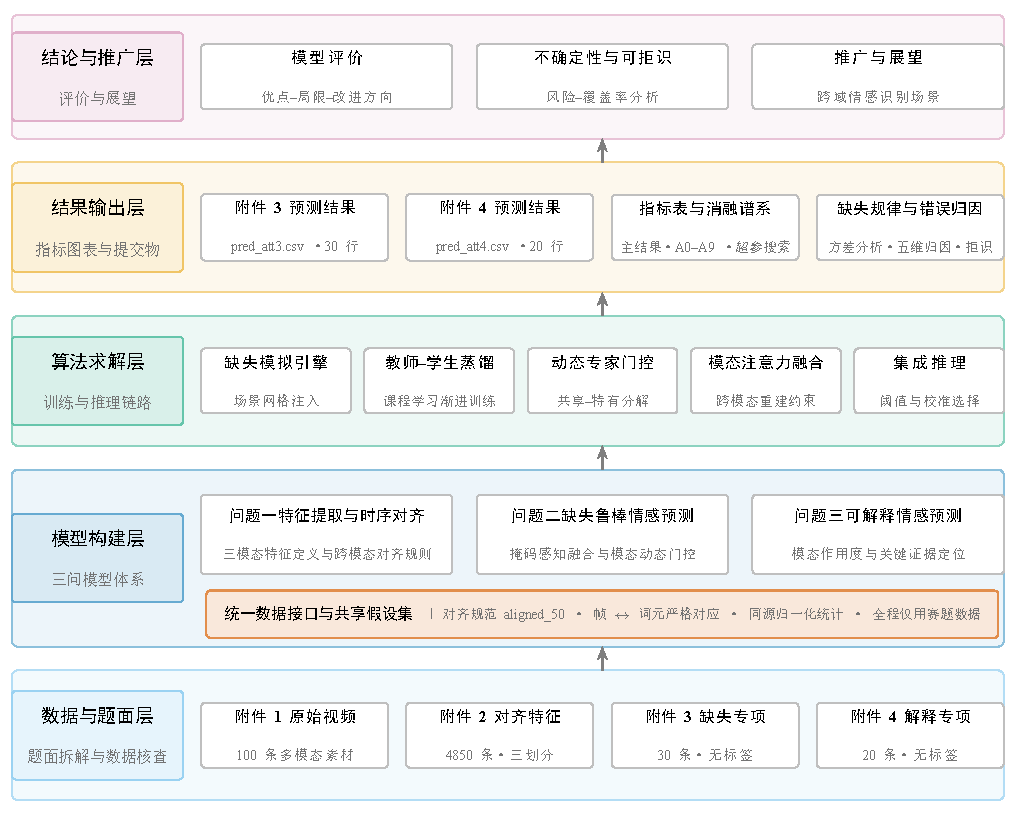
\includegraphics[width=0.95\textwidth]{tikz/总体架构图_五层建模框架.pdf}
  \caption{本文总体建模架构。全文自下而上分五层：数据与题面层完成四个附件的结构核查与统一读入；模型构建层为三项任务建立时序对齐、掩码感知鲁棒融合与可解释预测模型；算法求解层实现缺失模拟、课程学习与蒸馏、专家门控、注意力融合与集成推理；结果输出层给出预测文件、指标与消融谱系；结论与推广层完成评价与推广展望。}
  \label{fig:arch}
\end{figure}

架构图~\ref{fig:arch} 给出了全文的分层组织：三问共用第 1 层的输入接口与第 2 层的统一符号体系，差异体现在第 2 层的模型分支与第 3 层的求解环节。该结构保证了问题一产出的特征规范可直接被问题二、问题三复用，避免了三问之间口径漂移。

%% ------------------------------------------------------------------ 5
\section{模型建立与求解}

\subsection{问题一：多模态情感特征提取与时序对齐}
（本节为骨架占位：待补充特征定义、提取工具与参数、跨模态对齐规则、全量特征结果表与可复现说明。）

\subsection{问题二：模态缺失条件下的鲁棒情感预测}

问题二的求解链路共九个环节，从输入读入到提交文件输出的完整顺序如图~\ref{fig:q2flow} 所示。

\begin{figure}[H]
  \centering
  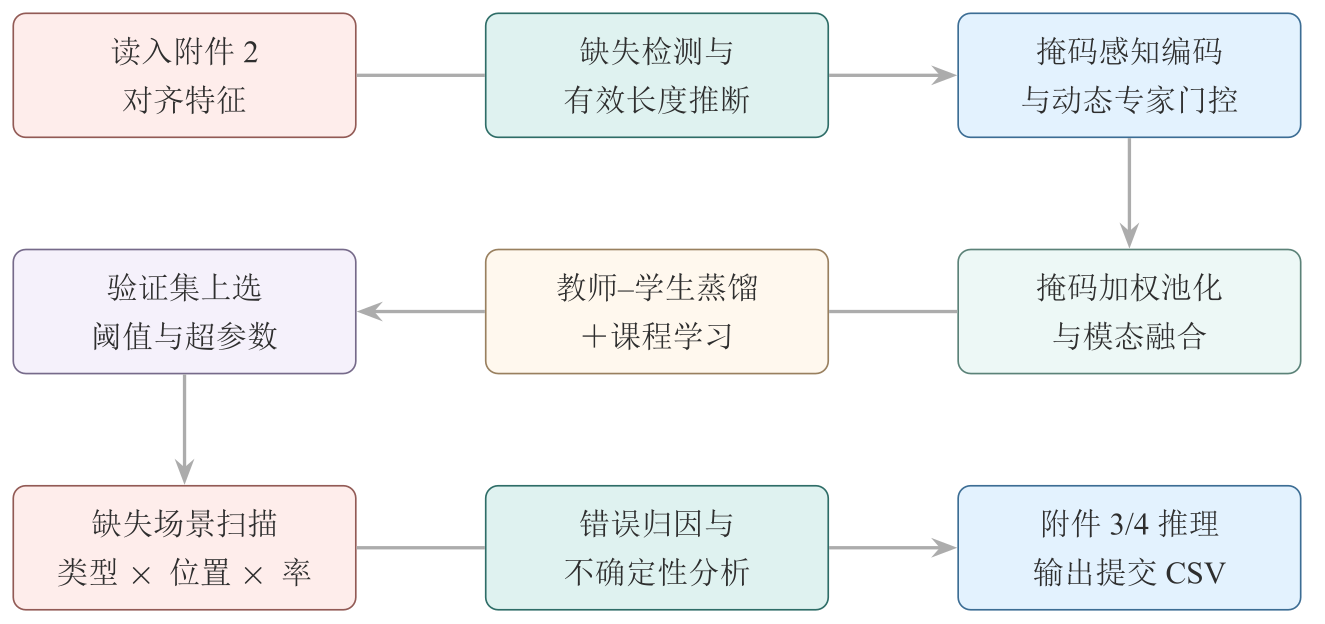
\includegraphics[width=0.94\textwidth]{figures/Q2_求解流程图.png}
  \caption{问题二求解流程（蛇形横向）。流程依次为读入对齐特征、缺失检测与有效长度推断、掩码感知编码与动态专家门控，折返后为掩码加权池化与模态融合、教师与学生蒸馏结合课程学习、验证集上选择阈值与超参数，再折返完成缺失场景网格扫描、错误归因与不确定性分析，最终输出附件三与附件四的提交文件。整体呈波浪式往复推进，下游环节只依赖上游产物。}
  \label{fig:q2flow}
\end{figure}

\subsubsection{输入表示与缺失掩码的数学定义}

设第 $m$ 模态的原始特征矩阵为 $\bm{X}_m\in\mathbb{R}^{T\times d_m}$，其中 $T=50$ 为统一对齐长度。填充掩码由尾部连续零值判定：

\begin{equation}
P_m(t)=\mathbf{1}\!\left[\sum_{\tau=t}^{T}\left\|\bm{X}_m(\tau)\right\|_1=0\right],
\label{eq:pad}
\end{equation}

有效长度随即由式~\eqref{eq:pad} 给出：

\begin{equation}
L_m=T-\sum_{t=1}^{T}P_m(t).
\label{eq:len}
\end{equation}

缺失掩码在有效区间内判定，要求连续不少于两帧全零：

\begin{equation}
M_m(t)=\mathbf{1}\!\left[P_m(t)=0\;\wedge\;\exists\,t_0\le t<t_1:\;
t_1-t_0\ge 2\;\wedge\;\sum_{\tau=t_0}^{t_1-1}\left\|\bm{X}_m(\tau)\right\|_1=0\right].
\label{eq:miss}
\end{equation}

模态缺失率定义为缺失帧数占有效长度的比例：

\begin{equation}
\rho_m=\frac{\sum_{t=1}^{T}M_m(t)}{L_m},
\label{eq:rho}
\end{equation}

当整条序列在有效区间内全零时规定 $\rho_m=1$。式~\eqref{eq:pad} 至式~\eqref{eq:rho} 构成了全文唯一使用的缺失口径，后续所有表格、图与提交文件均按此计算。

\subsubsection{掩码感知的模态编码}

模型由掩码判定、掩码感知编码、共享-特有分解、多尺度时间池化、动态专家门控与模态融合、多任务输出六个模块串联而成，三个模态各自走前四个模块后并入融合模块。整体结构如图~\ref{fig:q2net} 所示。

\begin{figure}[H]
  \centering
  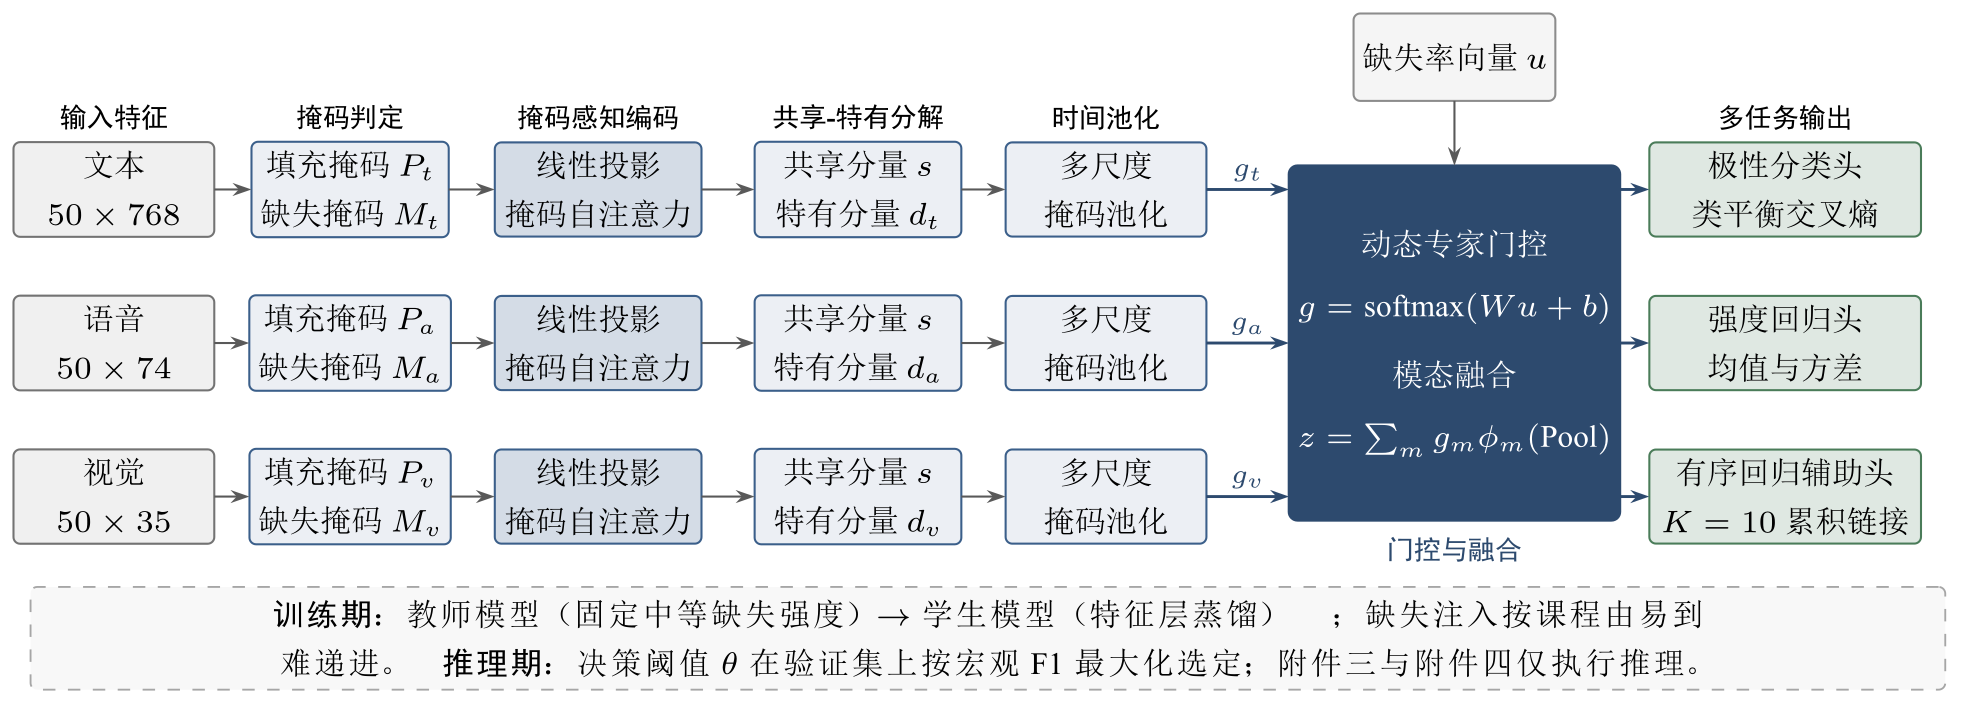
\includegraphics[width=\textwidth]{figures/Q2_网络结构图.png}
  \caption{问题二模型的网络结构。每个模态依次经过掩码判定、掩码感知编码、共享-特有分解与多尺度时间池化，四条纵向流程共享同一套参数设定；门控模块以三模态缺失率构成的向量为输入，输出样本级模态权重，融合结果再送入极性分类头、强度回归头与有序回归辅助头。该图与正文公式一一对应，训练期附加的蒸馏与课程学习见图中注记。}
  \label{fig:q2net}
\end{figure}

每个模态先经线性投影与位置编码映射到统一隐维度 $d$：

\begin{equation}
\bm{h}_m^{(0)}(t)=W_m^{\top}\bm{X}_m(t)+\bm{p}(t),\qquad
\bm{p}(t)\in\mathbb{R}^{d},
\label{eq:proj}
\end{equation}

随后由 $L_e$ 层自注意力编码，注意力计算中以填充与缺失的并集作为屏蔽项，使不可用时间步不参与信息聚合：

\begin{equation}
\mathrm{Attn}(\bm{Q},\bm{K},\bm{V})=\mathrm{softmax}\!\left(
\frac{\bm{Q}\bm{K}^{\top}}{\sqrt{d}}+\bm{B}\right)\bm{V},\qquad
B(t,\tau)=-\infty\cdot\mathbf{1}\!\left[P_m(\tau)=1\;\vee\;M_m(\tau)=1\right].
\label{eq:maskedattn}
\end{equation}

为刻画模态间的共性与个性，编码后的表示按共享-特有方式分解：

\begin{equation}
\bm{e}_m(t)=\bm{s}(t)+\bm{d}_m(t),
\label{eq:sharespec}
\end{equation}

其中 $\bm{s}(t)$ 为三模态共享分量，$\bm{d}_m(t)$ 为第 $m$ 模态的特有分量。该分解使缺失条件下来自不同模态的信息可在共享子空间内互补。

\subsubsection{动态专家门控与模态融合}

样本级模态权重由门控网络按缺失模式自适应生成。将各模态缺失率、总体填充比例与视觉有效帧数比拼接为门控输入：

\begin{equation}
\bm{u}=\big[\rho_{\mathrm{t}},\rho_{\mathrm{a}},\rho_{\mathrm{v}},
\bar{P},\;n_{\mathrm{v}}/3\big],
\label{eq:gatein}
\end{equation}

门控权重为

\begin{equation}
g_m=\frac{\exp\!\big(w_m^{\top}\bm{u}+b_m\big)}{\sum_{m'}\exp\!\big(w_{m'}^{\top}\bm{u}+b_{m'}\big)}.
\label{eq:gate}
\end{equation}

式~\eqref{eq:gate} 的关键在于权重随缺失模式变化，而非对所有样本使用固定权重。为避免专家退化到少数模态，引入负载均衡正则：

\begin{equation}
\mathcal{L}_{\mathrm{bal}}=\sum_{m}\left(\bar{g}_m-\frac{1}{3}\right)^2,
\label{eq:balance}
\end{equation}

其中 $\bar{g}_m$ 为批内该模态门控权重的均值。融合表示为

\begin{equation}
\bm{z}=\sum_{m}g_m\,\phi_m\!\big(\mathrm{Pool}(\bm{e}_m)\big),
\label{eq:fusion}
\end{equation}

式中 $\mathrm{Pool}$ 为掩码加权的多尺度时间池化，仅在有效且未缺失的时间步上求和：

\begin{equation}
\mathrm{Pool}(\bm{e}_m)=\frac{\sum_{t=1}^{T}\big(1-P_m(t)\big)\big(1-M_m(t)\big)\bm{e}_m(t)}
{\sum_{t=1}^{T}\big(1-P_m(t)\big)\big(1-M_m(t)\big)+\epsilon}.
\label{eq:pool}
\end{equation}

本文的融合与训练设计可与题目给定文献逐项对照。动态专家门控与 EMOE 的“模态专属动态情感专家”目标一致\cite{ref17}，
差别在于本文门控的输入显式包含三模态缺失率与填充比例。教师--学生蒸馏对应 CMAD 的模态感知蒸馏\cite{ref12}，
本文额外把缺失类型与缺失率作为课程维度。超图条件扩散\cite{ref10} 与 Proxy-Driven 方法\cite{ref13} 分别以生成式补全与
代理任务应对不完整数据，本文不做跨模态生成，而以掩码参与注意力、缺失注入与对数方差头达到同类目的。与
“分解--重建--增强”框架\cite{ref11} 相比，本文保留共享-特有分解但停用重建项（关闭后验证集误差由 0.5871 降至 0.5825），
该负结果已在消融一节如实报告；其余文献对应本文的选题依据与稳健性动机\cite{ref9,ref14,ref16,ref18}。

\subsubsection{目标函数}

强度回归采用带方差的负对数似然，使模型同时输出预测均值与预测方差：

\begin{equation}
\mathcal{L}_{\mathrm{reg}}=\frac{1}{N}\sum_{i=1}^{N}
\left[\frac{\big(y_i-\mu_i\big)^2}{2\sigma_i^2}+\frac{1}{2}\ln\sigma_i^2\right].
\label{eq:nll}
\end{equation}

极性分类采用类平衡交叉熵，类权重取类频倒数并作截断：

\begin{equation}
\mathcal{L}_{\mathrm{cls}}=-\frac{1}{N}\sum_{i=1}^{N}
\omega_{c_i}\sum_{k=0}^{2}\mathbf{1}\!\left[c_i=k\right]\ln\pi_{i,k},\qquad
\omega_k\propto\frac{1}{n_k},
\label{eq:ce}
\end{equation}

式中 $\omega_k$ 截断于区间 $[0.2,10]$ 以抑制极端类权重。跨模态重建约束要求由两模态预测第三模态，且对缺失时间步不施加惩罚：

\begin{equation}
\mathcal{L}_{\mathrm{rec}}=\sum_{m}\frac{\sum_{t}\big(1-P_m(t)\big)\big(1-M_m(t)\big)
\left\|\hat{\bm{X}}_m(t)-\bm{X}_m(t)\right\|_2^2}
{\sum_{t}\big(1-P_m(t)\big)\big(1-M_m(t)\big)+\epsilon}.
\label{eq:rec}
\end{equation}

式~\eqref{eq:rec} 的重建项属于搜索起点引入的辅助约束。消融实验表明移除该项后验证集误差与宏观 F1 同时改善，故最终配方将其权重置零（见消融实验一节），此处保留完整定义以便复现整个搜索过程。

为强化共享-特有分解的可辨识性，引入相似性约束与正交性约束：

\begin{equation}
\mathcal{L}_{\mathrm{sim}}=\sum_{m}\left\langle\bar{\bm{s}},\bar{\bm{d}}_m\right\rangle^{2},
\qquad
\mathcal{L}_{\mathrm{orth}}=\sum_{m\ne m'}\left\langle\bar{\bm{d}}_m,
\bar{\bm{d}}_{m'}\right\rangle^{2}.
\label{eq:simorth}
\end{equation}

此外引入有序回归辅助项。将强度绝对值离散为 $K=10$ 档，档位为 $k=\mathrm{round}(3|y|)$，以累积链接方式对 $K-1$ 个累积事件作二分类：

\begin{equation}
\mathcal{L}_{\mathrm{CORAL}}=-\frac{1}{N(K-1)}\sum_{i=1}^{N}\sum_{j=0}^{K-2}
\Big[\tilde{k}_i>j\Big]\ln\varsigma_{i,j}+\Big[\tilde{k}_i\le j\Big]\ln\big(1-\varsigma_{i,j}\big),
\label{eq:coral}
\end{equation}

其中 $\varsigma_{i,j}=\mathrm{sigmoid}\big(w^{\top}\bm{z}_i+b_j\big)$ 为累积概率，阈值 $\{b_j\}$ 为可学习参数。训练期的缺失注入按课程学习方式由易到难递进，第 $e$ 轮注入缺失率的上下界为

\begin{equation}
\rho_{\min}(e)=\rho_0+\big(\rho_1-\rho_0\big)\frac{e}{E},\qquad
\rho_{\max}(e)=\rho_1\,\frac{e}{E},
\label{eq:curriculum}
\end{equation}

式中 $E$ 为学生阶段总轮数。教师模型在固定中等缺失强度下训练，学生模型通过特征层蒸馏学习教师的软标签：

\begin{equation}
\mathcal{L}_{\mathrm{KD}}=\mathrm{KL}\!\left(
\mathrm{softmax}\big(\bm{o}^{T}/\tau\big)\,\big\|\,
\mathrm{softmax}\big(\bm{o}^{S}/\tau\big)\right),
\label{eq:kd}
\end{equation}

其中 $\tau$ 为蒸馏温度。总损失为各项加权和：

\begin{equation}
\mathcal{L}=\mathcal{L}_{\mathrm{reg}}+\lambda_1\mathcal{L}_{\mathrm{cls}}
+\lambda_2\mathcal{L}_{\mathrm{rec}}+\lambda_3\mathcal{L}_{\mathrm{sim}}
+\lambda_4\mathcal{L}_{\mathrm{orth}}+\lambda_5\mathcal{L}_{\mathrm{bal}}
+\lambda_6\mathcal{L}_{\mathrm{CORAL}}+\lambda_7\mathcal{L}_{\mathrm{KD}}.
\label{eq:total}
\end{equation}

\subsubsection{决策阈值选择与校准}

题目规定决策阈值在验证集上选择。本文采用单一对称阈值：当预测强度 $\hat{y}<-\theta$ 判为负类，$|\hat{y}|\le\theta$ 判为中性，$\hat{y}>\theta$ 判为正类。阈值按验证集 Macro-F1 最大化确定：

\begin{equation}
\theta^{\star}=\arg\max_{\theta\in\Theta}\;
\mathrm{MacroF1}\!\left(\big\{\mathrm{polar}(\hat{y}_i,\theta)\big\},\{c_i\}\right),\qquad
\Theta=\{0,0.02,\dots,1.50\}.
\label{eq:theta}
\end{equation}

由于强度分数存在系统性收缩，本文同时给出仿射校准作为对照，其系数同样仅在验证集上估计：

\begin{equation}
\big(\alpha^{\star},\beta^{\star}\big)=\arg\min_{\alpha,\beta}
\frac{1}{|\mathcal{V}|}\sum_{i\in\mathcal{V}}\left|\alpha\mu_i+\beta-y_i\right|.
\label{eq:calib}
\end{equation}

按题目规定，若校准后验证集分类指标不占优，则主口径不采用校准，仅列为敏感性分析。

\subsubsection{训练方案与关键参数}

式~\eqref{eq:total} 中各项权重与网络容量均在验证集上逐项比较后确定，最终配方汇总于表~\ref{tab:q2hparam}
与表~\ref{tab:q2hparam2}。表中所列取值与代码配置文件逐项对应，可作为复现依据。


\begin{table}[H]
\centering
  \caption{问题二模型的损失权重、缺失课程与决策参数。各类损失权重中的 $\lambda$ 编号与式~\eqref{eq:total} 一致，便于对照阅读。需要说明的是重建项权重取零，即最终配方未启用跨模态重建，其依据见消融实验一节。决策阈值只在验证集上确定，附件三与附件四不参与选择。}
\label{tab:q2hparam2}
\small
\begin{tabular}{@{}p{2.85cm}p{3.75cm}p{3.05cm}p{4.65cm}@{}}
\toprule
参数 & 取值 & 参数 & 取值 \\
\midrule
$\lambda_1$ 分类 & 1.0 & 方差项 & 0.1 \\
SmoothL1 的 $\beta$ & 0.15 & $\lambda_2$ 重建 & 0，未启用 \\
$\lambda_3$ 相似 & 0.5 & $\lambda_4$ 正交 & 0.5 \\
$\lambda_5$ 负载均衡 & 0.01 & $\lambda_6$ 有序回归 & 0.5，$K=10$ \\
$\lambda_7$ 蒸馏初始 & 0.3 & 蒸馏温度与预热 & 2.0，3 轮 \\
蒸馏衰减轮数 & 15 & 弱标注加权 & $\alpha=0.5$ \\
中性抑制 & 0.25 & 位置先验 & 中 $4/9$，头 $3/9$，尾与随机各 $1/9$ \\
课程第 1 至 8 轮 & 缺失率 $[0,0.10]$，单模态 & 课程第 9 至 20 轮 & 缺失率 $[0.04,0.20]$，多模态混合 \\
课程第 21 轮起 & 缺失率 $[0.04,0.25]$，多模态混合 & 决策阈值 & 网格 $\{0,0.02,\dots,1.50\}$，按验证集宏观 F1 最大 \\
\bottomrule
\end{tabular}
\end{table}

\begin{table}[H]
\centering
  \caption{问题二模型的数据、网络与训练参数。容量、正则强度、缺失注入课程与优化设置均在验证集上逐项比较后选定，表中同时给出缺失判定的连续零帧阈值与时间裁剪的保留比例，用于核对代码实现是否与论文中的定义一致，这两处设置直接决定缺失与填充能否被正确区分。}
\label{tab:q2hparam}
\small
\begin{tabular}{@{}p{3.25cm}p{4.15cm}p{3.15cm}p{4.15cm}@{}}
\toprule
参数 & 取值 & 参数 & 取值 \\
\midrule
特征版本与序列长度 & aligned，$T=50$ & 隐维度 & $d=96$ \\
缺失判定 & 有效区间内连续 $\ge2$ 帧全零 & 门控专家数 & $n_E=2$ \\
注意力 & 头数 4，编码层数 2 & 轮数 & 教师 12，学生 14 \\
丢弃率与权重衰减 & 0.35，$5\times10^{-4}$ & 批大小与优化器 & 64，AdamW 配余弦退火 \\
学习率 & 主干 $5\times10^{-5}$，头 $5\times10^{-4}$ & 梯度裁剪与早停 & 1.0，耐心 8 轮 \\
输入噪声与整模态丢弃 & 0.15，0.15 & 标签平滑与权重平均 & 0.1，指数移动平均 0.99 \\
缺失片段数与裁剪保留 & 每模态 1 至 3 段，保留 0.7 & 位置先验 & 中 $4/9$，头 $3/9$，尾与随机各 $1/9$ \\
\bottomrule
\end{tabular}
\end{table}

两张表中重建项权重取零这一设置并非初值，而是在验证集上比较后作出的取舍：消融实验中关闭该项反而使误差下降，故最终配方中将其停用，相关证据见消融实验一节。

\subsubsection{求解结果}

模型在验证集上的基础性能列于表~\ref{tab:q2main}。分类指标以分类头为主口径，强度指标选用平均绝对误差、皮尔逊相关系数与一致性相关系数。

\begin{table}[H]
\centering
  \caption{问题二模型的基础性能。验证集为主报口径，测试划分仅作泛化核验，分类指标取分类头主口径。模型在验证集取得准确率 0.6223、宏观 F1 0.6158，在测试划分提升至 0.6534 与 0.6338，说明未在验证集上过拟合；中性类 F1 明显低于负类与正类，是主要的性能短板，也是后续归因分析的起点。}
\label{tab:q2main}
\begin{tabular}{lcccccc}
\toprule
划分 & MAE & Pearson & CCC & ACC & Macro-F1 & 中性类 F1 \\
\midrule
验证集（主报） & 0.5866 & 0.6543 & 0.6278 & 0.6223 & 0.6158 & 0.5056 \\
测试划分（核验） & 0.6216 & 0.6807 & 0.6515 & 0.6534 & 0.6338 & 0.4656 \\
\bottomrule
\end{tabular}
\end{table}

由表~\ref{tab:q2main} 可见，模型在验证集取得 ACC 0.6223 与 Macro-F1 0.6158，测试划分为 0.6534 与 0.6338，说明未过拟合；按分类头概率构造的二分类口径准确率为 0.8514，与文献在同数据集全模态设定下的 0.84 至 0.86 区间一致。中性类 F1 显著低于负类与正类，是最主要短板，其成因在归因分析中定位。

由于训练样本规模不同，本文指标与公开结果不可直接比较：赛题附件二提供训练样本 3395 条，公开 CMU-MOSEI 划分为
16326 条（约为其 $1/4.8$），且特征与划分口径均不同。按统一复现口径，公开基线的三分类准确率为 0.661 至 0.676、平均绝对误差为 0.526 至 0.601、
皮尔逊相关为 0.683 至 0.778，本文对应为 0.6223、0.5866 与 0.6543；二分类口径 0.8514 略高于
公开区间 0.778 至 0.841 的上沿，三分类与误差指标的 4 至 5 个百分点差距主要来自训练规模与划分差异
（明细见 \texttt{paper\_tables/lit\_vs\_ours.csv}）。

模型的强度预测行为可由预测值与真值的对应关系直接观察：样本在对角线附近聚集说明整体方向正确，但在两端明显向内收缩，负类平均偏差为 $+0.54$、正类平均偏差为 $-0.45$，属条件均值回归的固有性质。

强度预测与真值的对应关系见图~\ref{fig:q2scatter}。

\begin{figure}[H]
  \centering
  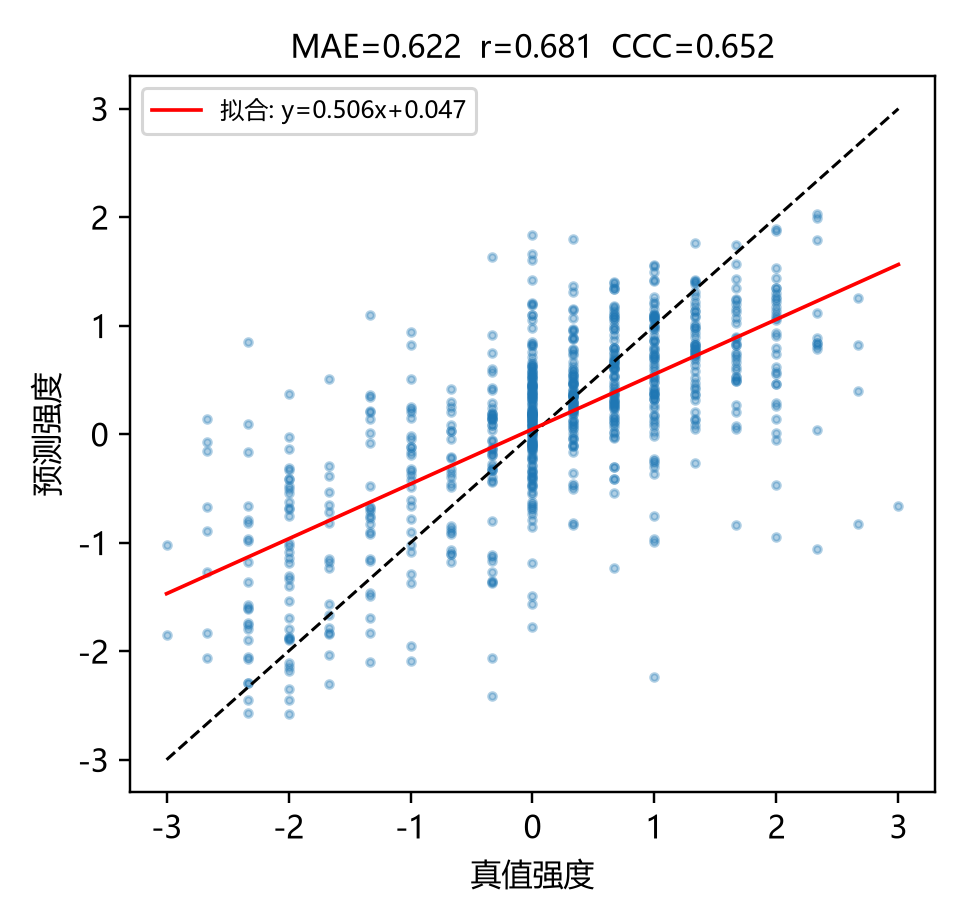
\includegraphics[width=0.78\textwidth]{figures/Q2_强度预测与真值散点_散点图.png}
  \caption{情感强度预测值与真值的散点分布。横轴为真值强度，纵轴为模型预测强度，虚线为恒等参考线。样本在对角线附近聚集说明模型整体方向正确，但在两端明显向内收缩：真值位于正负两端的样本被系统性地预测得不够极端。该收缩的量化表现是负类平均偏差 $+0.54$、正类平均偏差 $-0.45$，属于条件均值回归的固有性质。}
  \label{fig:q2scatter}
\end{figure}
强度误差只能说明回归头的表现，极性判别的好坏需要另看混淆结构。把验证集 728 条样本的预测极性与真值极性交叉统计可得：真中性 184 条中有 72 条被判为极性，同时有 147 条极性样本被判为中性，导致中性类精确率仅 0.4324；负类与正类的识别较为可靠。矩阵的非对角元直接指出错判的方向与规模，说明中性边界是当前模型的主要误差来源。

三分类混淆矩阵见图~\ref{fig:q2cm}。

\begin{figure}[H]
  \centering
  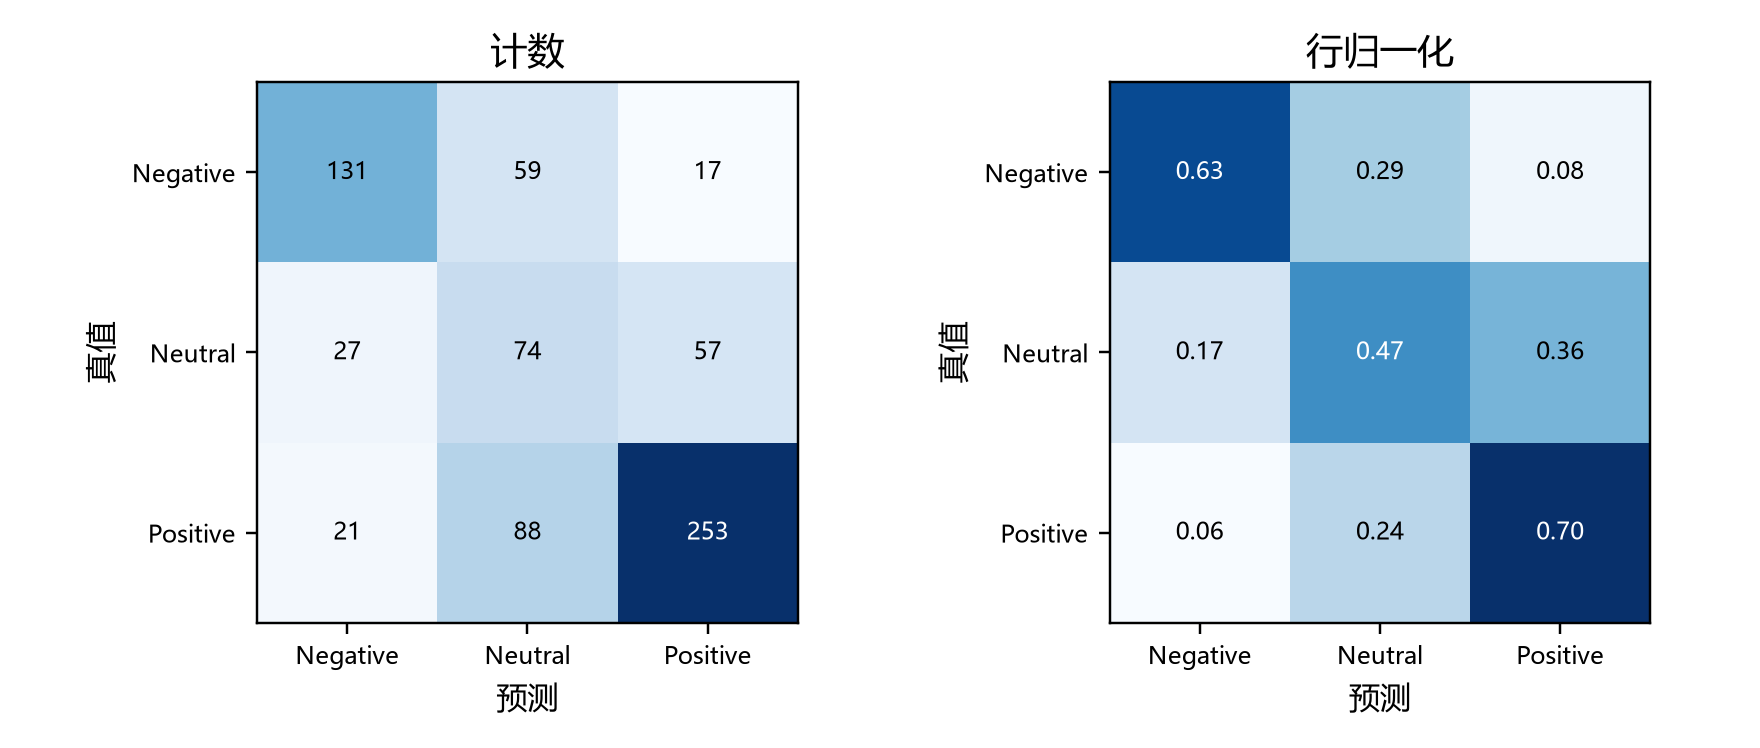
\includegraphics[width=0.62\textwidth]{figures/Q2_最终模型混淆矩阵_混淆矩阵.png}
  \caption{情感极性三分类混淆矩阵（验证集）。对角线为正确分类数，非对角线为混淆数，数值为样本数。负类与正类的识别较为可靠，中性类存在明显的双向混淆：真中性 184 条中有 72 条被判为极性，同时有 147 条极性样本被判为中性，导致中性类精确率仅 0.4324。该结果说明中性边界是当前模型的主要误差来源。}
  \label{fig:q2cm}
\end{figure}
极性判定不依赖单一阈值：在 $0.2$ 至 $0.4$ 区间内，验证集准确率与宏观 F1 变化平缓，并在阈值 $0.28$ 附近同时接近峰值。填充与缺失在本数据上同样可分离：填充判定成片出现在序列尾部且单调连续，缺失判定只出现在有效区间内部，与式~\eqref{eq:pad}、式~\eqref{eq:miss} 的分离规则一致；若把填充计为缺失，缺失率将被高估约一倍。

缺失掩码与填充掩码的时序可视化见图~\ref{fig:q2mask}。

\begin{figure}[H]
  \centering
  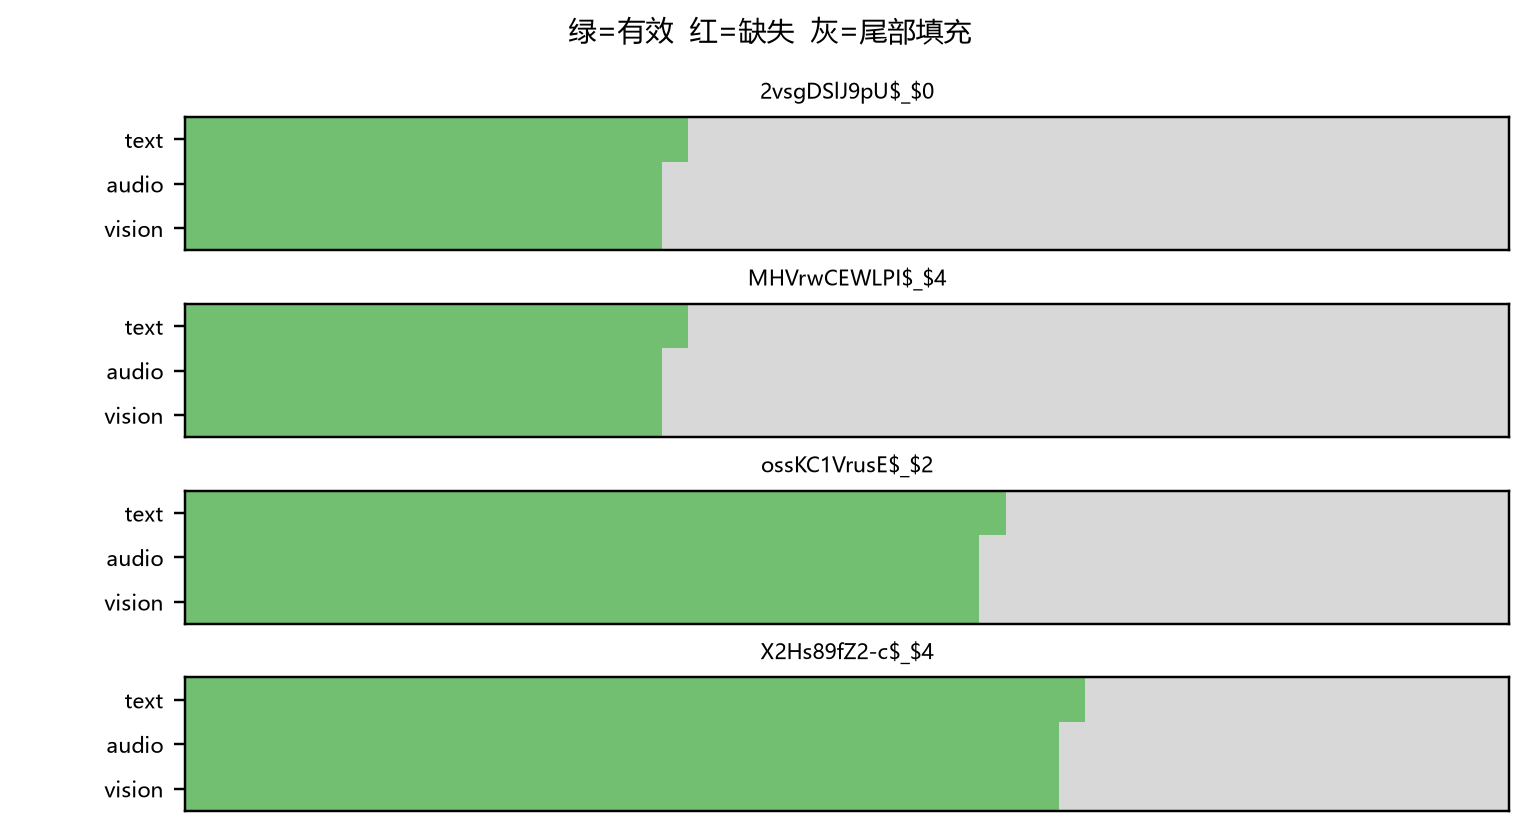
\includegraphics[width=0.72\textwidth]{figures/Q2_缺失掩码可视化_时序图.png}
  \caption{缺失掩码与填充掩码的时序可视化。横向条带表示时间步，颜色区分有效帧、填充帧与缺失帧。填充帧成片出现在序列尾部且单调连续，缺失帧则出现在有效区间内部；两者在图中共现但不重叠，验证了式~\eqref{eq:pad} 与式~\eqref{eq:miss} 的分离规则。该图同时说明若把填充计为缺失，缺失率将被高估约一倍。}
  \label{fig:q2mask}
\end{figure}

阈值敏感性曲线见图~\ref{fig:q2theta}。

\begin{figure}[H]
  \centering
  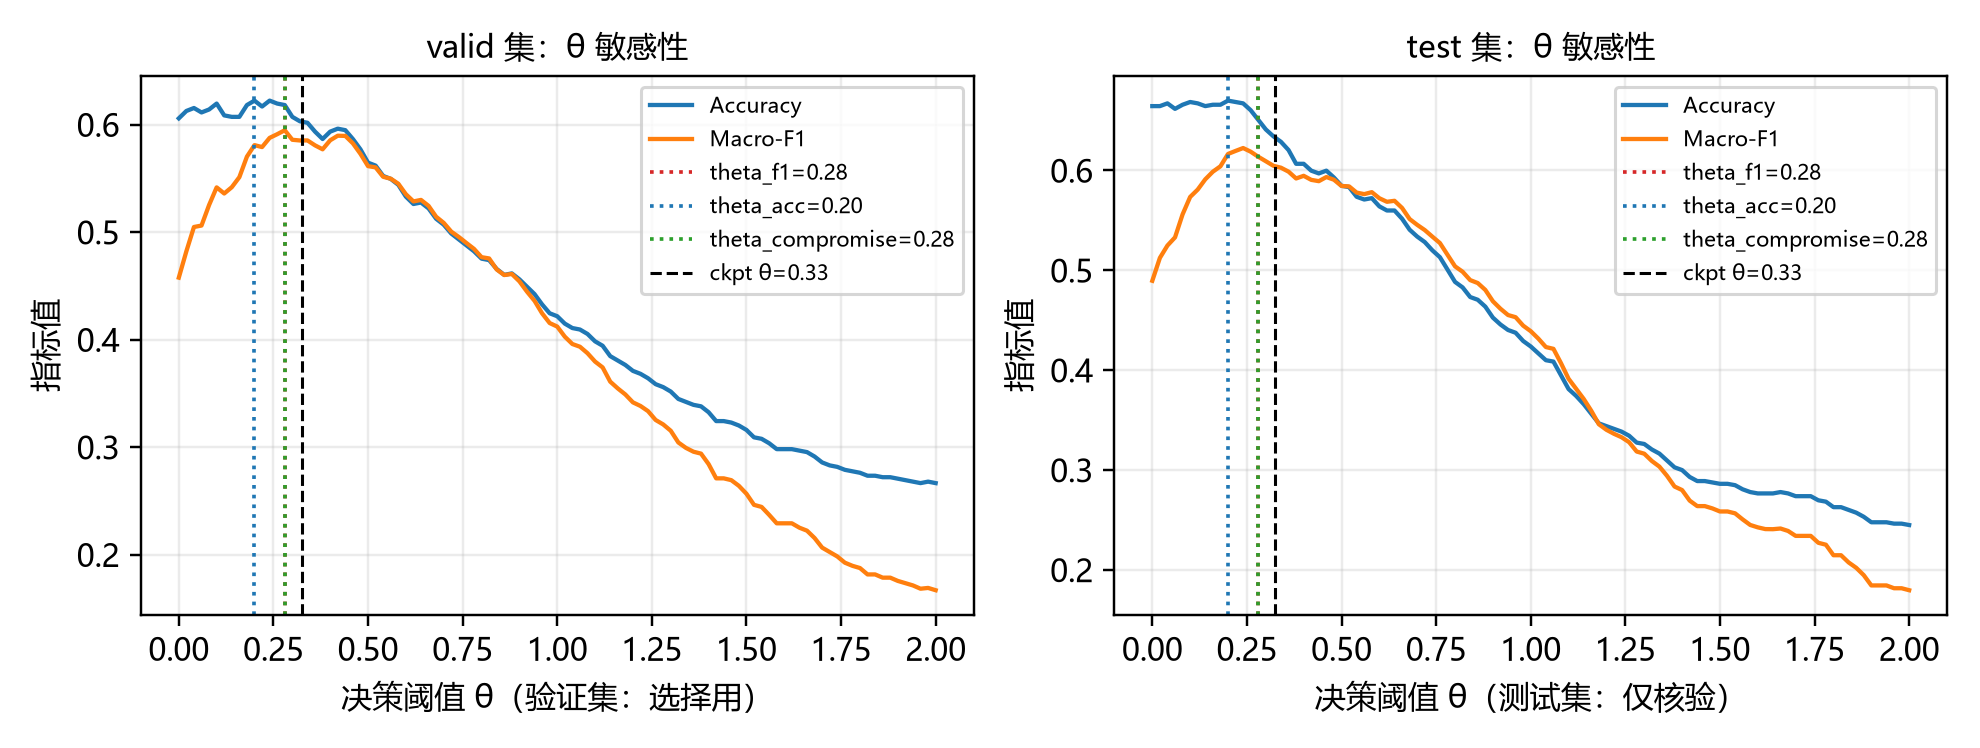
\includegraphics[width=0.72\textwidth]{figures/Q2_决策阈值敏感性曲线_折线图.png}
  \caption{决策阈值的敏感性曲线。横轴为阈值，纵轴为验证集准确率与宏观 F1，两条曲线在阈值 0.28 附近同时接近峰值。曲线在 0.2 至 0.4 区间变化平缓，说明两个准则选出的阈值一致且对扰动不敏感；由于阈值只在验证集上确定，该图同时作为口径合规性的证据。}
  \label{fig:q2theta}
\end{figure}
\subsubsection{缺失因素影响规律}

为分析缺失类型、位置与时长对性能的影响，本文构造三维场景网格：缺失类型取 6 种组合（文本、语音、视觉、文本加语音、语音加视觉、三模态），缺失位置取头部、中部、尾部、随机 4 种，缺失率取 0.1 至 1.0 共 5 档，合计 120 个场景。缺失率按式~\eqref{eq:rho} 定义，即缺失帧数占该模态有效长度的比例；不直接以绝对帧数分档，是因为三种模态的有效长度差异很大（文本恒为 50 帧，语音与视觉约 24.6 与 23.8 帧），同一绝对档位在不同模态与样本上对应的缺失比例可相差数倍。

性能退化量定义为相对无缺失基线的差值：

\begin{equation}
\Delta\mathrm{MAE}(\tau,p,\rho)=\mathrm{MAE}\big(\tau,p,\rho\big)-\mathrm{MAE}_{\mathrm{clean}},
\qquad
\Delta\mathrm{ACC}=\mathrm{ACC}\big(\tau,p,\rho\big)-\mathrm{ACC}_{\mathrm{clean}}.
\label{eq:delta}
\end{equation}

各缺失类型下的退化曲线随缺失率的变化见图~\ref{fig:q2degrade}。

\begin{figure}[H]
  \centering
  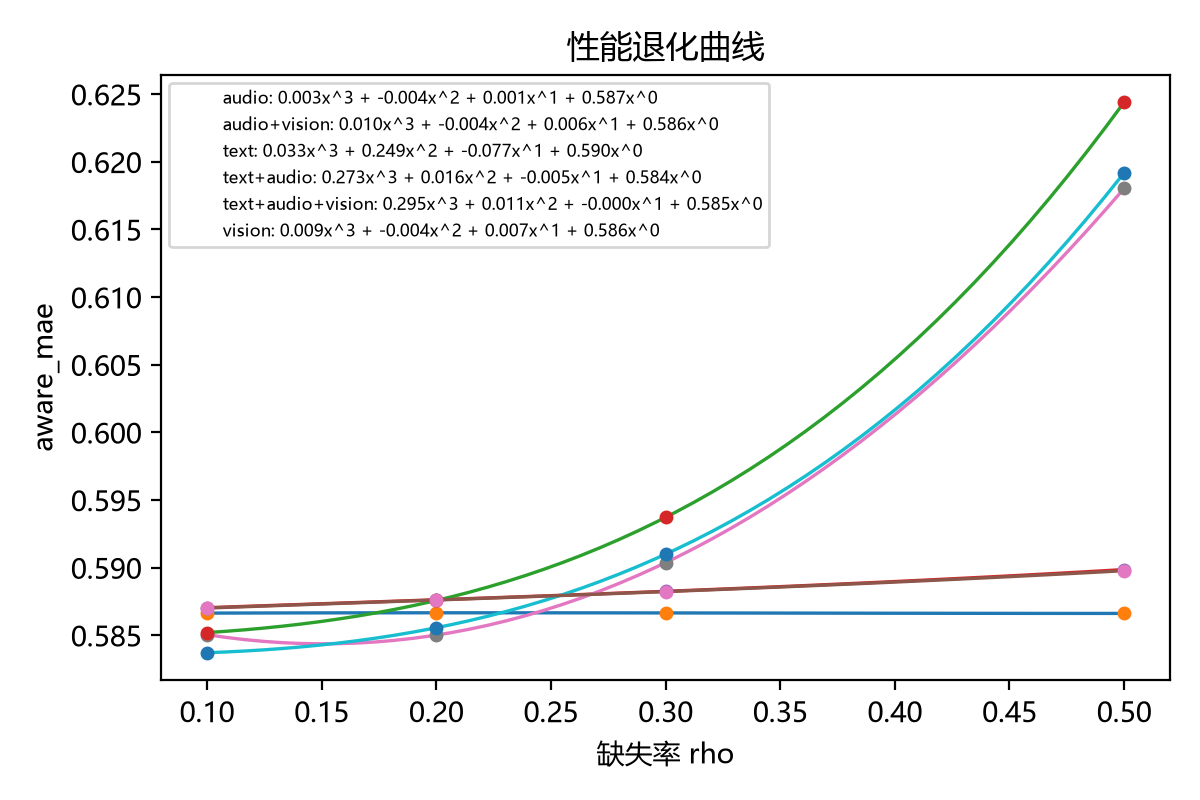
\includegraphics[width=0.68\textwidth]{figures/Q2_缺失退化MAE曲线_折线图.png}
  \caption{各缺失类型下的退化曲线。横轴为注入缺失率，纵轴为平均绝对误差，多条曲线按缺失类型区分。文本类缺失曲线在缺失率超过 0.3 后快速上升，缺失率达到 1.0 时误差由 0.5866 升至约 0.77；而语音与视觉类缺失曲线在整个区间内近乎水平。该对比直接说明本任务的退化由文本模态驱动。}
  \label{fig:q2degrade}
\end{figure}

交叉缺失类型与缺失位置两个维度后，可得退化的二维分布：文本类所在的整行明显深于语音与视觉行，其中头部缺失的误差增量最高；语音与视觉行在全列上数值接近零，说明这两类模态的缺失位置对结果几无影响。

缺失类型与缺失位置的退化热力图见图~\ref{fig:q2heat}。

\begin{figure}[H]
  \centering
  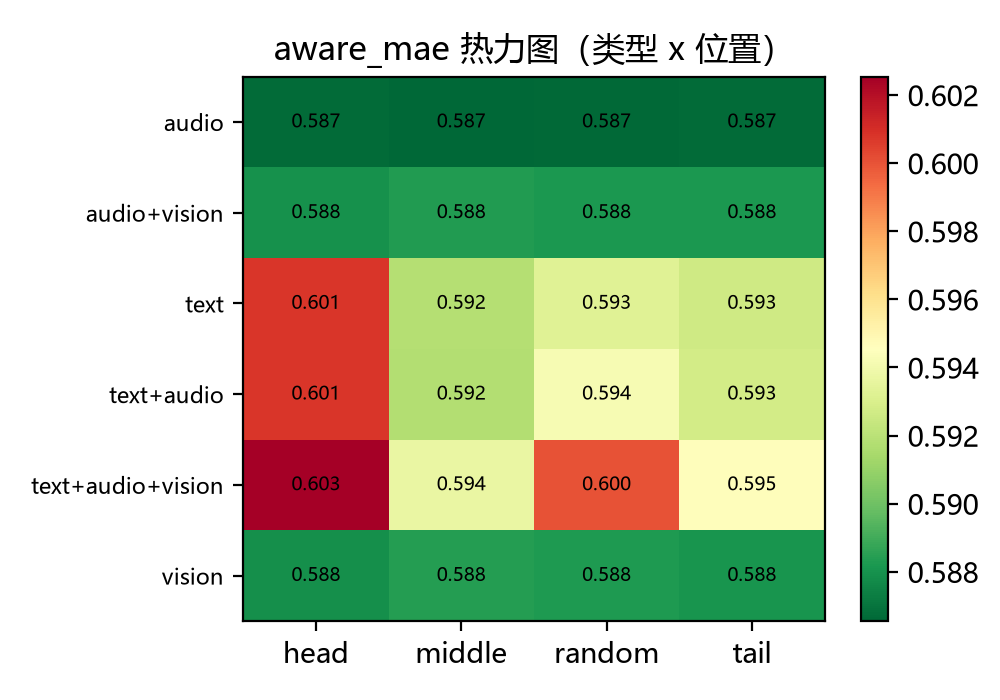
\includegraphics[width=0.68\textwidth]{figures/Q2_模态类型-缺失位置热力图_热力图.png}
  \caption{缺失类型与缺失位置的退化热力图。行表示缺失类型，列表示缺失位置，单元格数值为相对基线的误差增量，颜色越深表示退化越严重。文本类所在的整行明显深于语音与视觉行，其中头部缺失格的数值最高。语音与视觉行在全列上数值接近零，说明这两类模态的缺失位置对结果几无影响。}
  \label{fig:q2heat}
\end{figure}
为进一步量化本文处理相对基线方案的收益，本文把四个模型置于同一退化扫描协议下对比。两个朴素融合基线代表不做缺失处理的常规做法，另两个为本文模型的单种子与集成版本，结果见图~\ref{fig:q2cmp}。

\begin{figure}[H]
  \centering
  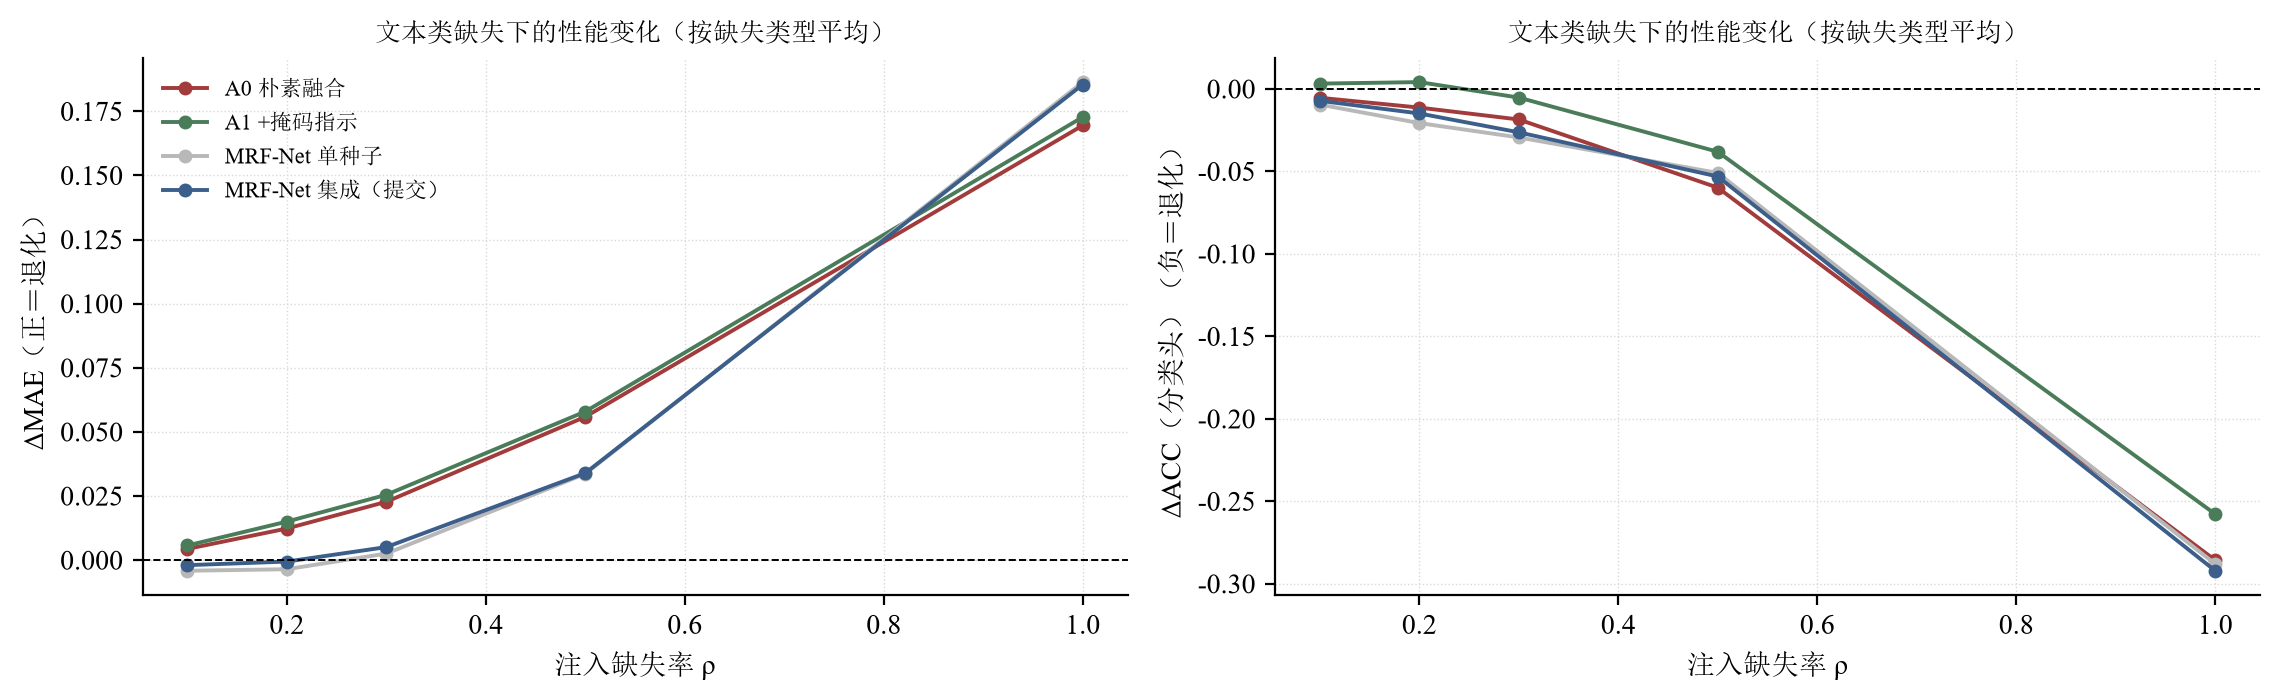
\includegraphics[width=0.95\textwidth]{figures/Q2_四模型缺失退化对比_折线图.png}
  \caption{四个模型在文本类缺失下的性能对比。左图为误差增量随缺失率的变化，右图为准确率增量随缺失率的变化，虚线为零基准。两个朴素融合基线在缺失率 0.3 后误差快速上升，而本文模型与集成模型的曲线明显更低且更平缓。按位置平均，本文模型把退化降低 1.5 至 3.3 倍，其中头部场景收益最小，因为头部缺失本身就是最难恢复的情形。}
  \label{fig:q2cmp}
\end{figure}

退化曲线与缺失位置结构共同刻画了退化的主导因素。按缺失类型平均，语音缺失在缺失率 1.0 时的误差增量仅 0.0002，视觉缺失为 0.0068，两者合计 0.0071，而文本缺失达到 0.1804，约为前者的 25 倍。这说明本任务的情感判别以文本为主导模态，鲁棒性设计的重点应集中在文本分支。

上述比较建立在同一缺失率上，而同一缺失率在文本上对应的绝对时长约为语音与视觉的两倍，需排除时长口径的干扰。做法是挑出绝对缺失帧数相匹配的场景重比：缺失率 0.5 的文本（25.0 帧）对缺失率 1.0 的语音与视觉（24.59 与 23.82 帧），三者相差在 5\% 以内。匹配后按位置平均，文本缺失的误差增量为 $+0.0314$、语音 $+0.0002$、视觉 $+0.0068$，文本仍达语音的 170 倍；在约 5 帧的小缺失匹配组上（文本 0.1、语音 0.2、视觉 0.2），三维增量为 $-0.0016$、$+0.0001$、$+0.0010$，均接近零。可见退化由文本驱动并非来自时长口径差异。

为把上述定性判断量化为可检验的效应量，本文对退化量作三因素方差分析，响应变量取各场景相对基线的退化增量，误差项取最高阶交互：

\begin{equation}
\Delta\mathrm{MAE}\sim
C(\tau)\ast C(p)\ast C(\rho),
\label{eq:anova}
\end{equation}

其中 $C(\cdot)$ 表示按类别变量处理。各效应项的平方和占比即效应量 $\eta^2$，下文直接引用其数值。

各效应项的平方和占比即效应量 $\eta^2$，完整数值列于表~\ref{tab:anova}。

\begin{table}[H]
\centering
  \caption{三因素方差分析的效应量。响应变量为各场景相对无缺失基线的退化增量，缺失率区间取零到 0.5，误差项取最高阶交互。表中对比了朴素融合基线与本文模型：基线中缺失类型与缺失率的交互效应量高达 0.9517，本文模型降至 0.8415；同时缺失类型与缺失位置的交互由 0.0053 升至 0.0614。}
\label{tab:anova}
\begin{tabular}{lccl}
\toprule
效应项 & 朴素融合基线 $\eta^2$ & 本文模型 $\eta^2$ & 结论 \\
\midrule
缺失类型 $\times$ 缺失率 & 0.9517 & 0.8415 & 主导项，本文模型明显削弱 \\
缺失类型 $\times$ 缺失位置 & 0.0053 & 0.0614 & 本文模型开始利用位置信息 \\
缺失位置 $\times$ 缺失率 & 0.0025 & 0.0288 & 由位置信息引入 \\
缺失类型（主效应） & 0.0094 & 0.0081 & 次要 \\
缺失位置（主效应） & 0.0002 & 0.0041 & 可忽略 \\
缺失率（主效应） & 0.0004 & 0.0053 & 可忽略 \\
\bottomrule
\end{tabular}
\end{table}
从方差分析可得两条结论。其一，退化量几乎全部由缺失类型与缺失率的交互解释，基线模型该效应量高达 0.9517，本文模型降至 0.8415，说明缺失感知设计削弱了退化对缺失模式组合的依赖，把退化整体摊平。其二，缺失类型与缺失位置的交互效应量由 0.0053 升至 0.0614，提升约 12 倍，说明基线对缺失位置完全不敏感，而本文模型确实利用了位置信息，其残余退化呈现出位置结构。

进一步按位置边际化可得具体排序。排除整模态缺失情形后，本文模型在头部、中部、尾部、随机四种位置上的平均误差增量分别为 0.0078、0.0035、0.0039、0.0052，头部缺失最严重，约为中部的 2.2 倍；在文本模态上该差距扩大到 0.0141 对 0.0052，达 2.7 倍。基线模型四个位置的取值在 0.0102 至 0.0128 之间近乎持平，不呈现位置结构。

\subsubsection{消融实验}

为验证各模块的必要性，本文采用与超参搜索相同的配对方式：以消融基准配方为参照，保持种子与其余配置完全不变，逐项关闭模块后再比较，这样得到的差值只对应被关闭的那一个模块。需要说明的是，早期实验曾把另一套配方（隐维度 128、专家数 4、轮数更多且启用重建）当作对照，其差值被配方差异污染且部分行符号有误，本文已改用同配方对照，结果列于表~\ref{tab:ablation}。

\begin{table}[H]
\centering
  \caption{消融实验的验证集结果。前三行为基准配方在两种子上的取值及其极差，模块消融部分与种子 42 配对、只翻转一个开关，故差值只对应被关闭的那一个模块；下半部分为并列参照，配方或模型类型不同不做差。误差指标上任何模块的消融幅度都小于基准配方自身的种子极差，仅动态专家门控一项在宏观 F1 上略超过种子极差。}
\label{tab:ablation}
\small
\begin{tabular}{@{}lccccc@{}}
\toprule
配置 & 种子数 & MAE & 宏观 F1 & $\Delta$MAE & $\Delta$宏观 F1 \\
\midrule
基准配方（种子 42，配对基准） & 1 & 0.5871 & 0.5857 & --- & --- \\
基准配方（种子 43） & 1 & 0.5967 & 0.5765 & --- & --- \\
基准配方两种子极差 & 2 & --- & --- & 0.0095 & 0.0092 \\
\midrule
去除掩码指示 & 1 & 0.5866 & 0.5913 & $-0.0005$ & $+0.0056$ \\
去除跨模态重建 & 1 & 0.5825 & 0.5868 & $-0.0047$ & $+0.0011$ \\
单专家（去动态门控） & 1 & 0.5942 & 0.5733 & $+0.0070$ & $-0.0124$ \\
去除教师蒸馏 & 1 & 0.5913 & 0.5787 & $+0.0042$ & $-0.0070$ \\
去除缺失课程学习 & 1 & 0.5885 & 0.5898 & $+0.0013$ & $+0.0041$ \\
\midrule
朴素融合（无缺失处理） & 1 & 0.6010 & 0.5932 & --- & --- \\
朴素融合加掩码指示与缺失注入 & 1 & 0.5990 & 0.5782 & --- & --- \\
主模型（2 种子集成，最终配方） & 2 & 0.5866 & 0.6158 & --- & --- \\
\bottomrule
\end{tabular}
\end{table}

从表~\ref{tab:ablation} 可读出三条结论。第一，基准配方两种子之间的误差极差为 0.0095、宏观 F1 极差为 0.0092，而模块消融中幅度最大的移除动态专家门控也只有 0.0070，仍小于种子极差，说明单种子条件下误差指标无法判定模块贡献。第二，宏观 F1 上仅移除动态专家门控一项略超种子极差（0.0124 对 0.0092，约 1.35 倍），且误差与分类指标同向劣化，说明样本级模态加权确实在起作用；移除跨模态重建使两个指标同时改善，与最终配方关闭该项的设计决定一致。第三，两项朴素融合基线的误差分别高出基准 0.0139 与 0.0119，均已超过种子极差，而模块级消融均未做到，说明性能来源是缺失感知的整体框架，而非某一可单独摘除的模块。

表中最后一行给出最终部署的主模型作为参照。它与基准配方的差异包含关闭重建、引入有序回归辅助头与弱标注加权、调整轮数与启用权重平均等多项同时变化，验证集宏观 F1 由 0.5857 升至 0.6158。由于变动项不止一个，该提升不能归因于任一单项，故本文只将其列为参照而不做逐项分解。

结构选型分两阶段进行：先在训练子集上以较短轮数筛除明显劣化的候选，再对胜出者用全量训练集重训；候选覆盖容量、编码层数、专家数、正则强度与蒸馏权重五个方向。三条结论：以宏观 F1 排序时两阶段排名一致，说明短轮数筛选足以判断候选优劣方向；以平均绝对误差排序时出现反转（筛选阶段误差最低的隐维度 128 在完整训练后误差最高），原因是子集短轮数训练处于欠拟合区间，据此改用两个指标的并集挑选候选；各候选相对基线的差异大多落在单种子波动内（单种子标准差约为 0.0060 与 0.0083），仅隐维度由 96 增至 128 稳健地同时恶化两个指标（标准分 2.37 与 3.07），故最终配方保持隐维度 96 与蒸馏权重 0.3。

两阶段超参搜索的对比见图~\ref{fig:q2tune}。

\begin{figure}[H]
  \centering
  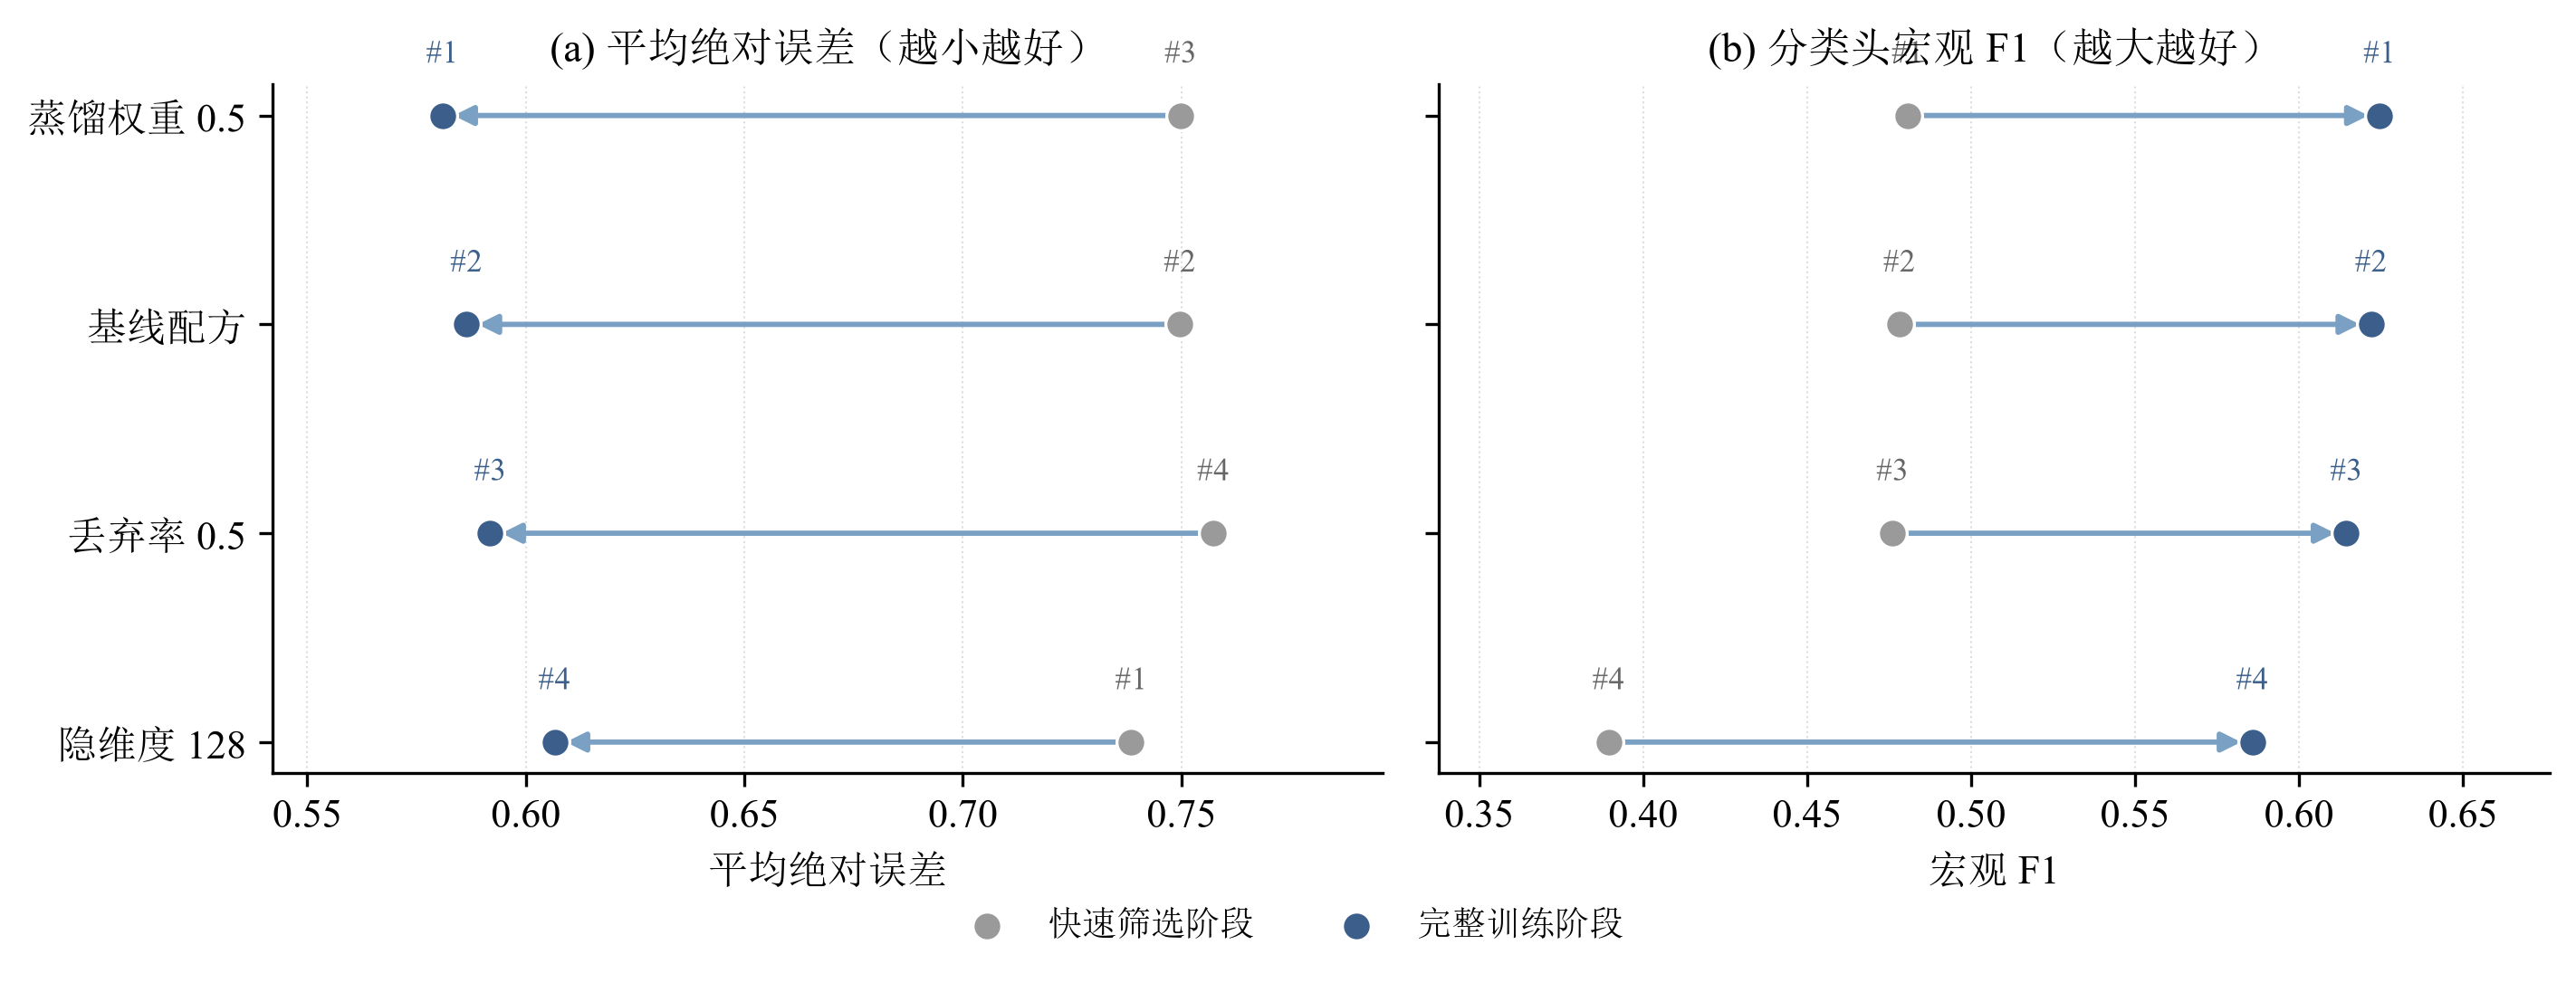
\includegraphics[width=0.98\textwidth]{figures/Q2_超参搜索screen与full对比_哑铃图.png}
  \caption{超参数搜索的快速筛选阶段与完整训练阶段对比（验证集，四个候选）。每个候选的两点由箭头连接，灰点为子集快速筛选结果，蓝点为全量训练结果，点旁数字为该阶段内的排名。宏观 F1 的排名在两阶段之间完全一致，而平均绝对误差的排名发生反转：筛选阶段误差最低的隐维度 128 配置，在完整训练后误差最高。}
  \label{fig:q2tune}
\end{figure}

\subsubsection{验证集可视化与错误归因}

强度绝对误差的分布存在明显长尾：多数样本误差小于 0.5，少数强情感样本超过 2.0，长尾样本主导了平均误差的量级。为定位误差来源，本文沿强度幅值、文本信息量、视觉信息量、极性类别与缺失状态五个维度分层统计，各分组的样本量、误差与分类准确率一并统计。

五维分层的完整结果见图~\ref{fig:q2errgroup}。

\begin{figure}[H]
  \centering
  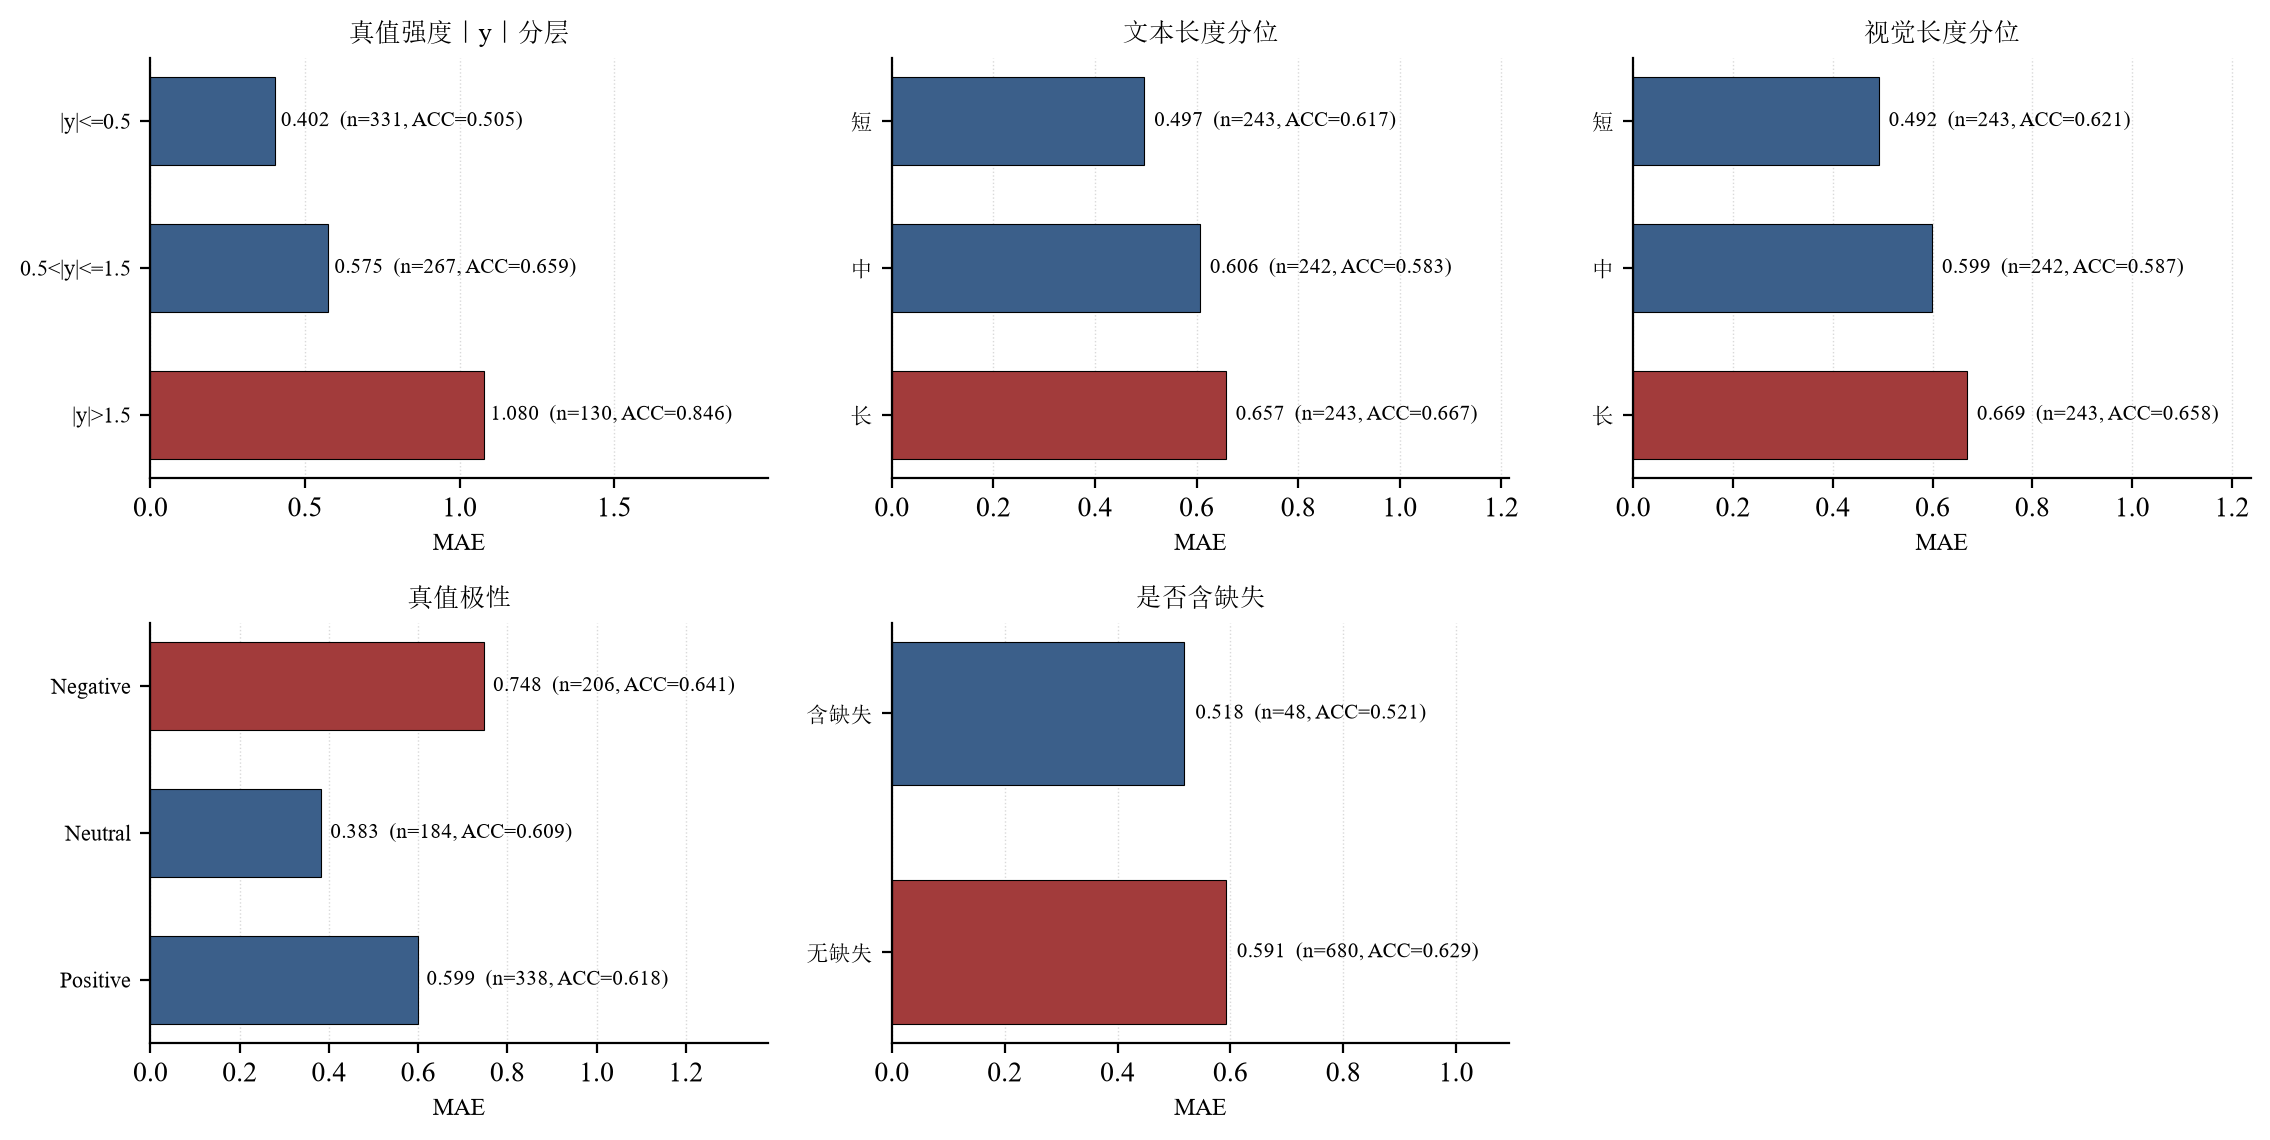
\includegraphics[width=0.95\textwidth]{figures/Q2_错误归因五维分层_条形图.png}
  \caption{错误归因的五维分层结果（验证集）。五个子图分别按真值强度、文本长度分位、视觉长度分位、真值极性与是否含缺失分层，条形长度表示平均绝对误差，并标注样本数与分类头准确率。按真值强度分层时误差随强度单调上升，明显高于其他维度；按极性分层时负类误差最高；含缺失子集的准确率显著低于无缺失子集。}
  \label{fig:q2errgroup}
\end{figure}

分组对比还显示出两个方向相反的现象：强度误差集中在强情感样本，而分类错误集中在弱强度样本。前者源于回归目标在分布极值处样本稀疏，后者源于三类边界附近的标签噪声与特征噪声难以分辨，因而同一模型在两个指标上呈现不同的易错区间。明确这一差异，可在后续应用中按场景选择强度的连续输出或极性的离散输出。绝对误差的分布形态见图~\ref{fig:q2errhist}。

\begin{figure}[H]
  \centering
  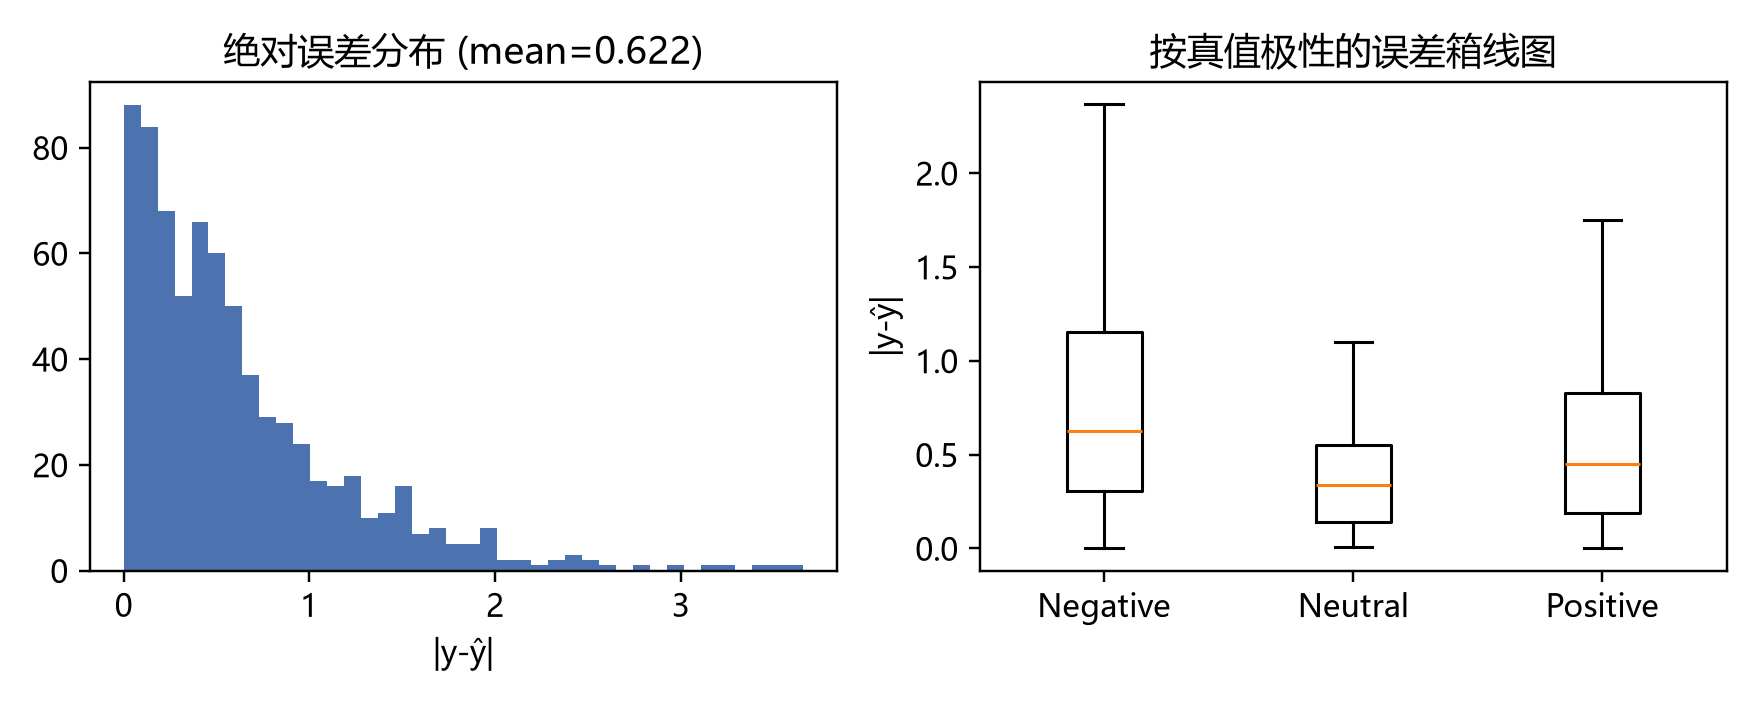
\includegraphics[width=0.66\textwidth]{figures/Q2_强度误差分布_直方图.png}
  \caption{情感强度绝对误差的分布直方图。横轴为绝对误差，纵轴为样本数，红色竖线为平均绝对误差的位置。分布在零点附近集中，但存在明显长尾：多数样本误差小于 0.5，少数强情感样本误差超过 2.0，长尾样本主导了平均误差，这一特征与后续分层归因的结论一致。}
  \label{fig:q2errhist}
\end{figure}
按真值强度分层可定位误差来源。绝对强度不超过 0.5 的样本占验证集的 45.5\%，平均绝对误差最低（0.402），但分类准确率仅 0.5045，接近随机水平；绝对强度超过 1.5 的样本平均绝对误差高达 1.080，分类准确率却达 0.8462。这说明强度误差集中在强情感样本（属回归目标的固有难度），极性误差集中在弱强度样本（属三分类边界难以刻画的问题）。

按真值极性分层则揭示了强度分数的系统性偏差。负类样本的平均偏差为正 0.541，即真实偏负的样本被系统性地预测得不够负；正类样本的平均偏差为负 0.447，方向相反；中性类样本偏差为 0.110。该现象与式~\eqref{eq:calib} 中校准斜率小于一的估计相互印证，是条件均值回归的必然结果。

含缺失子集的分类准确率为 0.521，比无缺失子集的 0.629 低 0.108，说明缺失确实损害了极性判别。但该子集在验证集中仅 48 条，测试划分中仅 40 条，样本量偏小，本文如实标注并不过度解读。

\subsubsection{不确定性分析与可拒识能力}

模型在式~\eqref{eq:nll} 中已输出预测方差，据此可定义两类不确定度。偶然不确定度取对数方差头输出的指数：

\begin{equation}
\sigma_{\mathrm{model}}=\exp\!\big(\ln\sigma^2/2\big),
\label{eq:aleatoric}
\end{equation}

认知不确定度由集成成员的分歧给出：

\begin{equation}
\sigma_{\mathrm{ens}}=\sqrt{\frac{1}{K-1}\sum_{k=1}^{K}\big(\mu_k-\bar{\mu}\big)^2},
\qquad
\sigma_{\mathrm{total}}=\sqrt{\sigma_{\mathrm{model}}^2+\sigma_{\mathrm{ens}}^2}.
\label{eq:epistemic}
\end{equation}

另一类与极性判别相关的不确定度取分类头概率熵：

\begin{equation}
H=-\sum_{k=0}^{2}\pi_k\ln\pi_k.
\label{eq:entropy}
\end{equation}

按不确定度升序保留前 $q$ 比例样本，可得风险--覆盖率曲线，其积分即 AURC：

\begin{equation}
\mathrm{AURC}=\int_{0}^{1}\mathrm{MAE}\big(q\big)\,\mathrm{d}q .
\label{eq:aurc}
\end{equation}

按不确定度剔除样本后误差与覆盖率的关系见图~\ref{fig:q2rc}。

\begin{figure}[H]
  \centering
  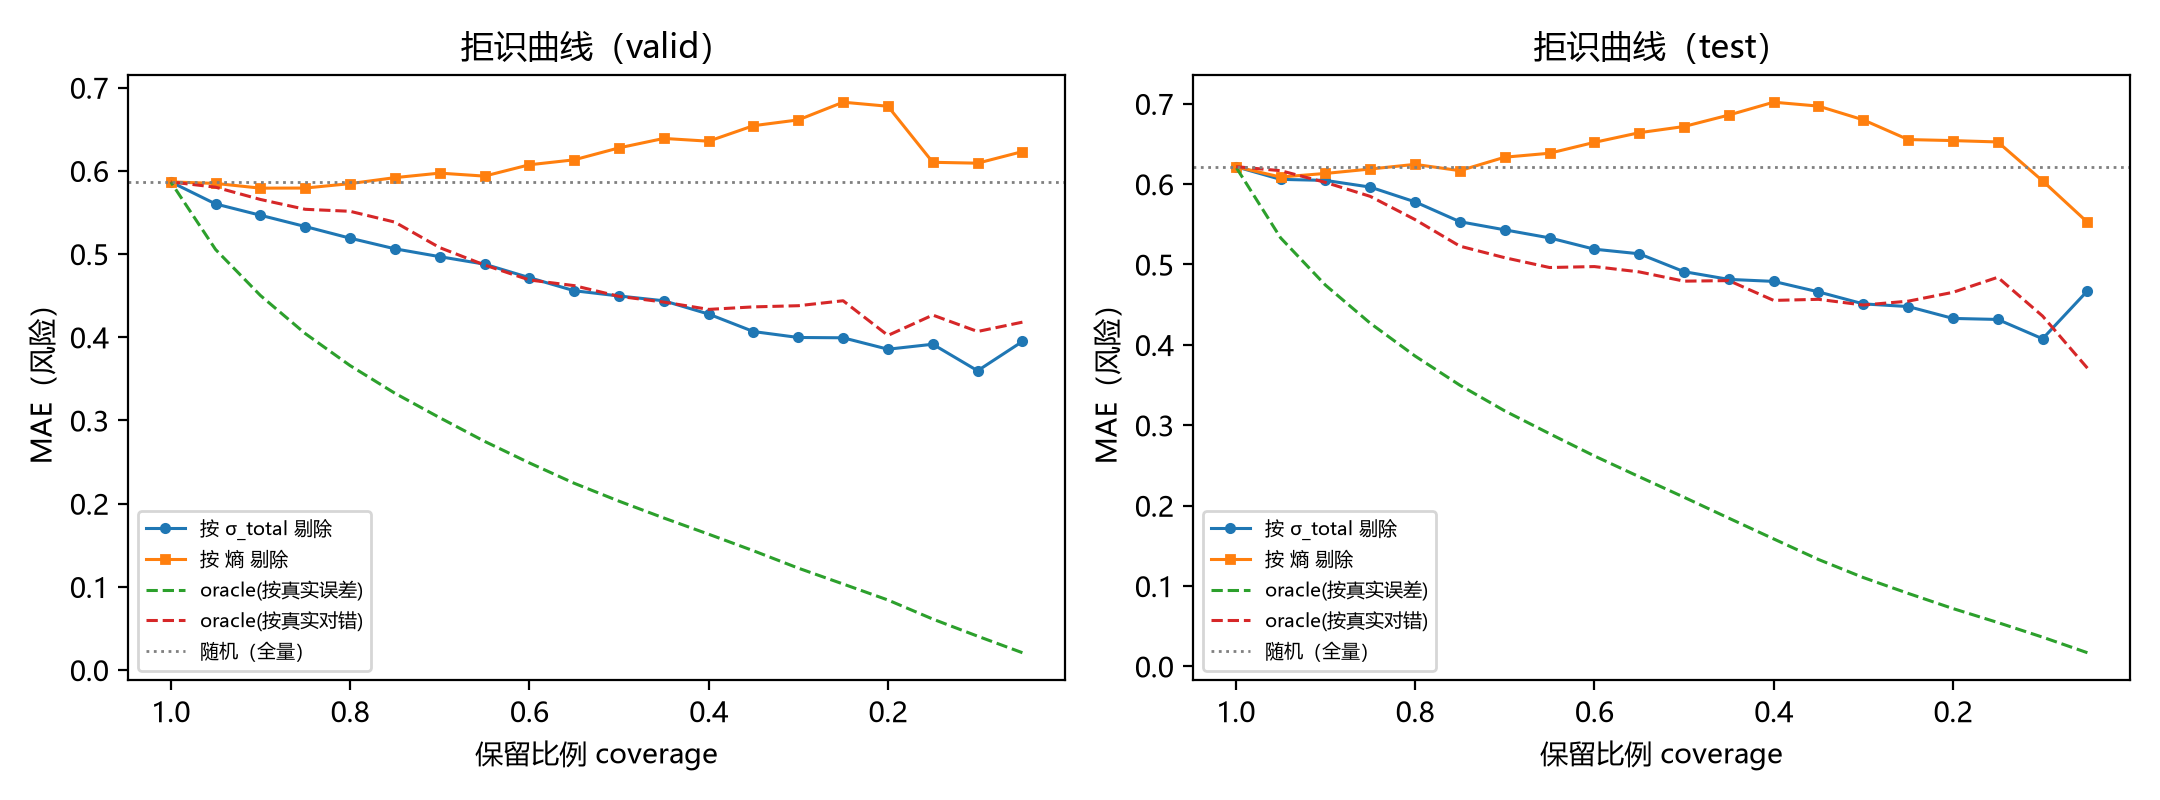
\includegraphics[width=0.95\textwidth]{figures/Q2_风险覆盖率曲线_折线图.png}
  \caption{风险覆盖率曲线（左验证集、右测试划分）。横轴为保留比例，纵轴为平均绝对误差，实线为按总不确定度剔除、点线为随机剔除、虚线为按真实误差剔除的理论下界。实线显著低于随机基线并接近下界，说明按总不确定度剔除不确定样本可有效降低误差。}
  \label{fig:q2rc}
\end{figure}

两类不确定度对分类准确率的影响方向并不一致。按总不确定度剔除会使准确率下降，而按分类头概率熵剔除则明显上升，两者的对比见图~\ref{fig:q2reject}。

\begin{figure}[H]
  \centering
  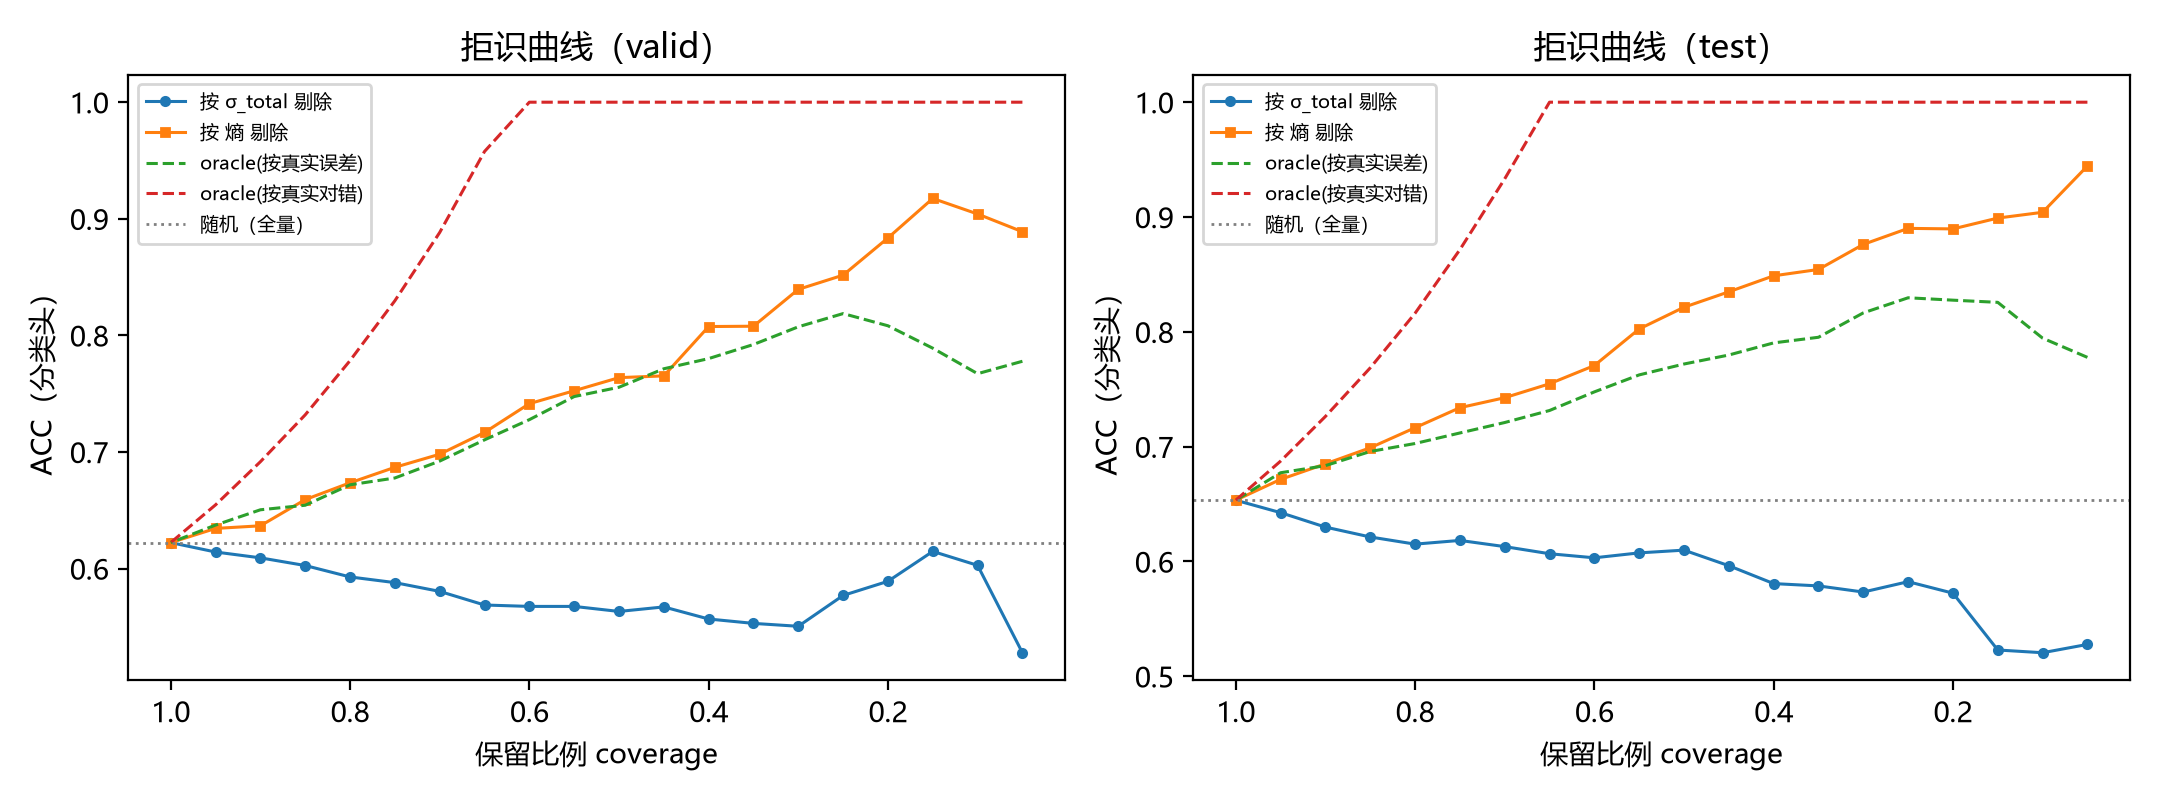
\includegraphics[width=0.95\textwidth]{figures/Q2_拒识对准确率影响_折线图.png}
  \caption{剔除最不确定样本对分类准确率的影响。横轴为保留比例，纵轴为分类头准确率。按总不确定度剔除时准确率反而下降，而按分类头概率熵剔除时准确率明显上升，保留一半样本时验证集准确率由 0.6223 升至 0.7637，测试划分升至 0.8214。该差异说明回归不确定度与分类不确定度是两个可分离的量，必须分别使用。}
  \label{fig:q2reject}
\end{figure}

总不确定度与绝对误差的逐样本关系见图~\ref{fig:q2unc}。横轴为集成成员分歧与对数方差头共同给出的总不确定度，纵轴为绝对强度误差，散点趋势与相关系数用于判定该不确定度是否可用于拒识。

\begin{figure}[H]
  \centering
  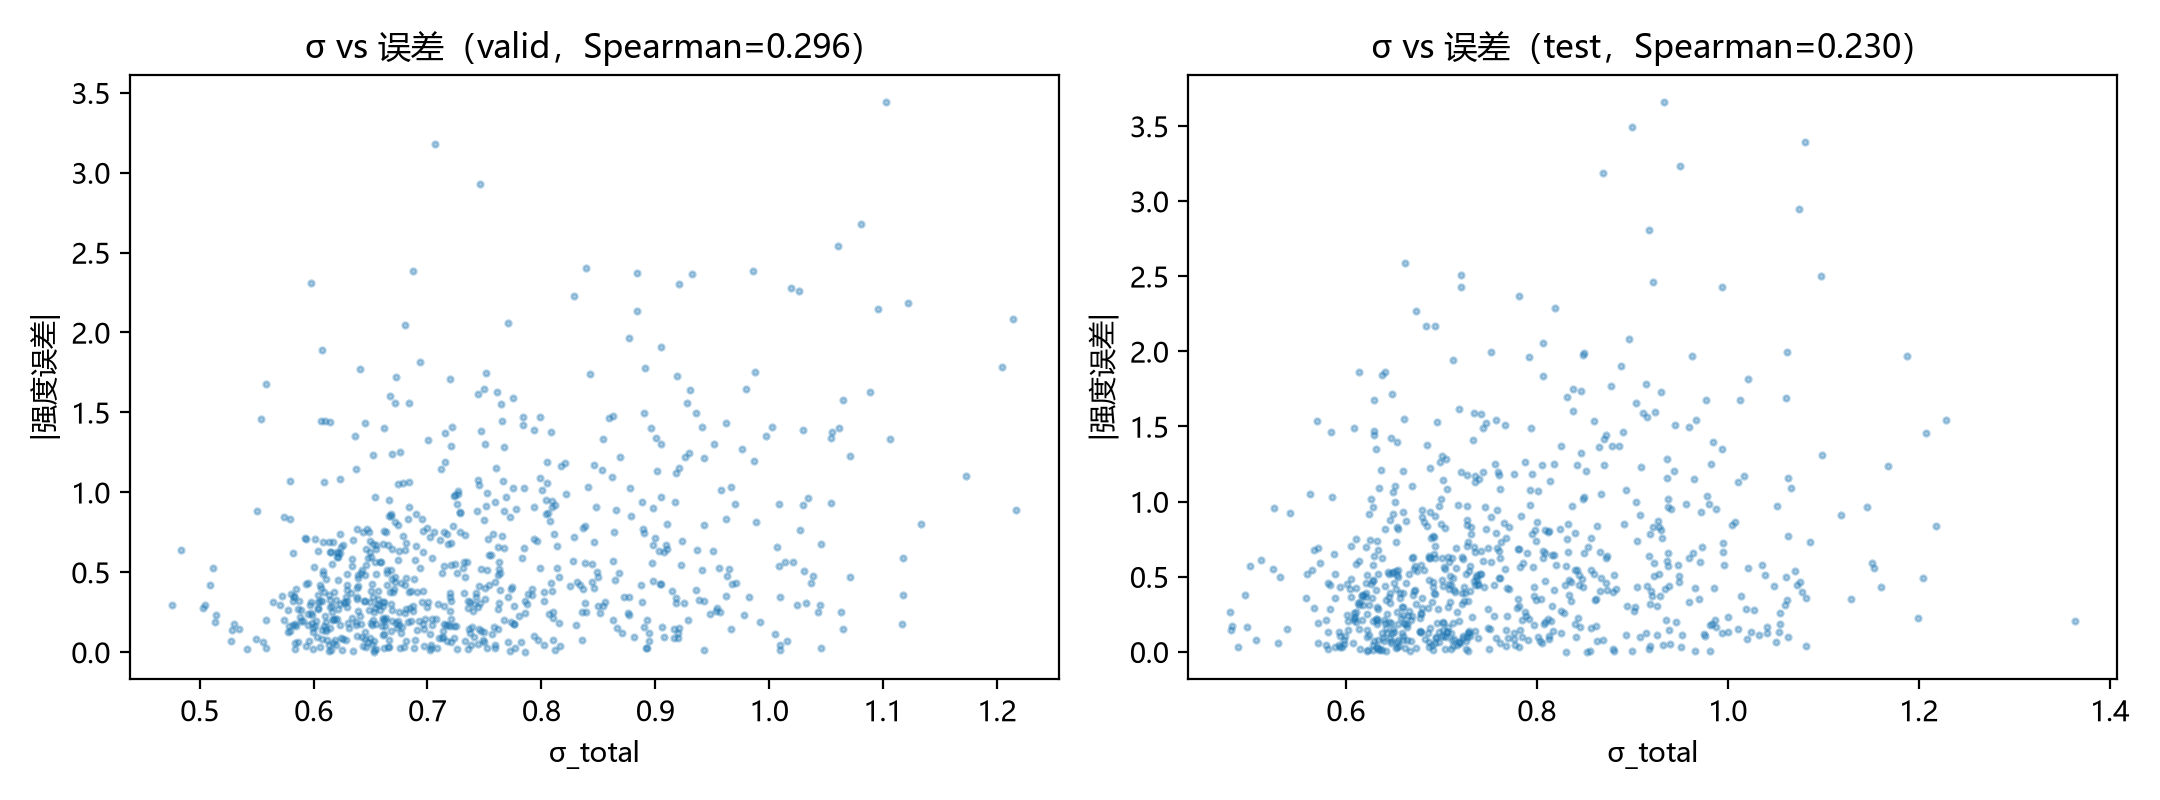
\includegraphics[width=0.95\textwidth]{figures/Q2_不确定度与误差关系_散点图.png}
  \caption{总不确定度与绝对误差的散点关系（左验证集、右测试划分）。横轴为总不确定度，纵轴为绝对强度误差，散点呈右上倾斜趋势，斯皮尔曼相关系数在验证集为 0.296、测试划分为 0.230，均为正且显著。这说明对数方差头输出的不确定度确实追踪了强度回归的误差幅值。}
  \label{fig:q2unc}
\end{figure}

风险覆盖率曲线~\ref{fig:q2rc} 至散点图~\ref{fig:q2unc} 给出定量结论。就强度回归而言，按总不确定度剔除最不确定的 10\% 样本后，平均绝对误差由 0.5866 降至 0.5465，剔除一半样本后降至 0.4495，风险覆盖率曲线下面积为 0.4365，而随机剔除的对应值为 0.5866、理论下界为 0.2258，说明所输出的不确定度具备实际拒识价值。就极性判别而言，按总不确定度剔除会使准确率下降，其风险覆盖曲线下面积 0.3980 甚至劣于随机的 0.3777；而改用分类头概率熵剔除时，曲线下面积降至 0.2252，远优于随机并接近理论下界 0.0828。

这一对比揭示了一个在文献中常被忽略的事实：用单一不确定度同时拒识回归与分类在本任务上并不成立。进一步的分层分析给出其机制。总不确定度与真值强度呈单调同增关系，按五分位分桶后，最确定一桶的真值绝对强度均值为 0.411，最不确定一桶为 1.233，说明总不确定度实质追踪的是情感强度幅值，因而对强度误差有信息、对极性误差反而反向。分类头概率熵则与强度呈递减关系，其追踪的是极性模糊度。据此本文把两类不确定度分别用于强度拒识与极性拒识，并报告了相应的收益。

\subsubsection{附件三与附件四的推理结果}

按题目的合规要求，附件三与附件四仅用于最终推理，不参与任何阈值或超参数选择。本文对两个测试集分别输出预测文件，并同步写入缺失率与缺失区间字段以便复核。

附件三 30 条样本的全量预测汇总列于表~\ref{tab:q2att3}。

\begin{table}[H]
\centering
  \caption{附件三测试集的全量预测汇总。极性同时给出分类头主口径与强度阈值口径，两组判定的样本一致率为 0.8333。含缺失子集指语音或视觉任一模态实测缺失率大于零的 18 条样本。含缺失子集的平均强度与平均绝对强度均低于无缺失子集，说明部分时段信息不可用时模型给出的预测更趋保守；两组平均置信度差异不足 0.03。}
\label{tab:q2att3}
\begin{tabular}{lccc}
\toprule
指标 & 全样本 & 含缺失 & 无缺失 \\
\midrule
样本数 & 30 & 18 & 12 \\
预测负向 & 6 & 4 & 2 \\
预测中性 & 14 & 10 & 4 \\
预测正向 & 10 & 4 & 6 \\
平均强度 & $+0.2451$ & $+0.1949$ & $+0.3204$ \\
平均绝对强度 & 0.4930 & 0.4304 & 0.5869 \\
平均置信度 & 0.5840 & 0.5738 & 0.5993 \\
两口径一致率 & 0.8333 & --- & --- \\
\bottomrule
\end{tabular}
\end{table}

从表~\ref{tab:q2att3} 可见，附件三的预测以中性与正向为主（中性 14 条），与该测试集的短片段构成相符。含缺失子集的平均强度为 $+0.1949$、平均绝对强度为 0.4304，均低于无缺失子集的 $+0.3204$ 与 0.5869，说明部分时段信息不可用时模型不仅方向上更趋保守，预测幅值也整体收缩；两组的平均置信度仅相差 0.026，表明缺失降低的是信息量而非模型对自身输出的信心。

预测极性构成与缺失状态的关系为：全样本负向 6 条、中性 14 条、正向 10 条，含缺失子集的负向与正向各 4 条，无缺失子集的半数为正向；预测强度集中在 $-1.2$ 至 $1.5$ 之间，置信度分布于 0.44 至 0.91 之间、均值 0.584，可用以核验提交文件中的分数与置信度字段无异常值。

预测强度与置信度的分布见图~\ref{fig:q2att3dist}。

\begin{figure}[H]
  \centering
  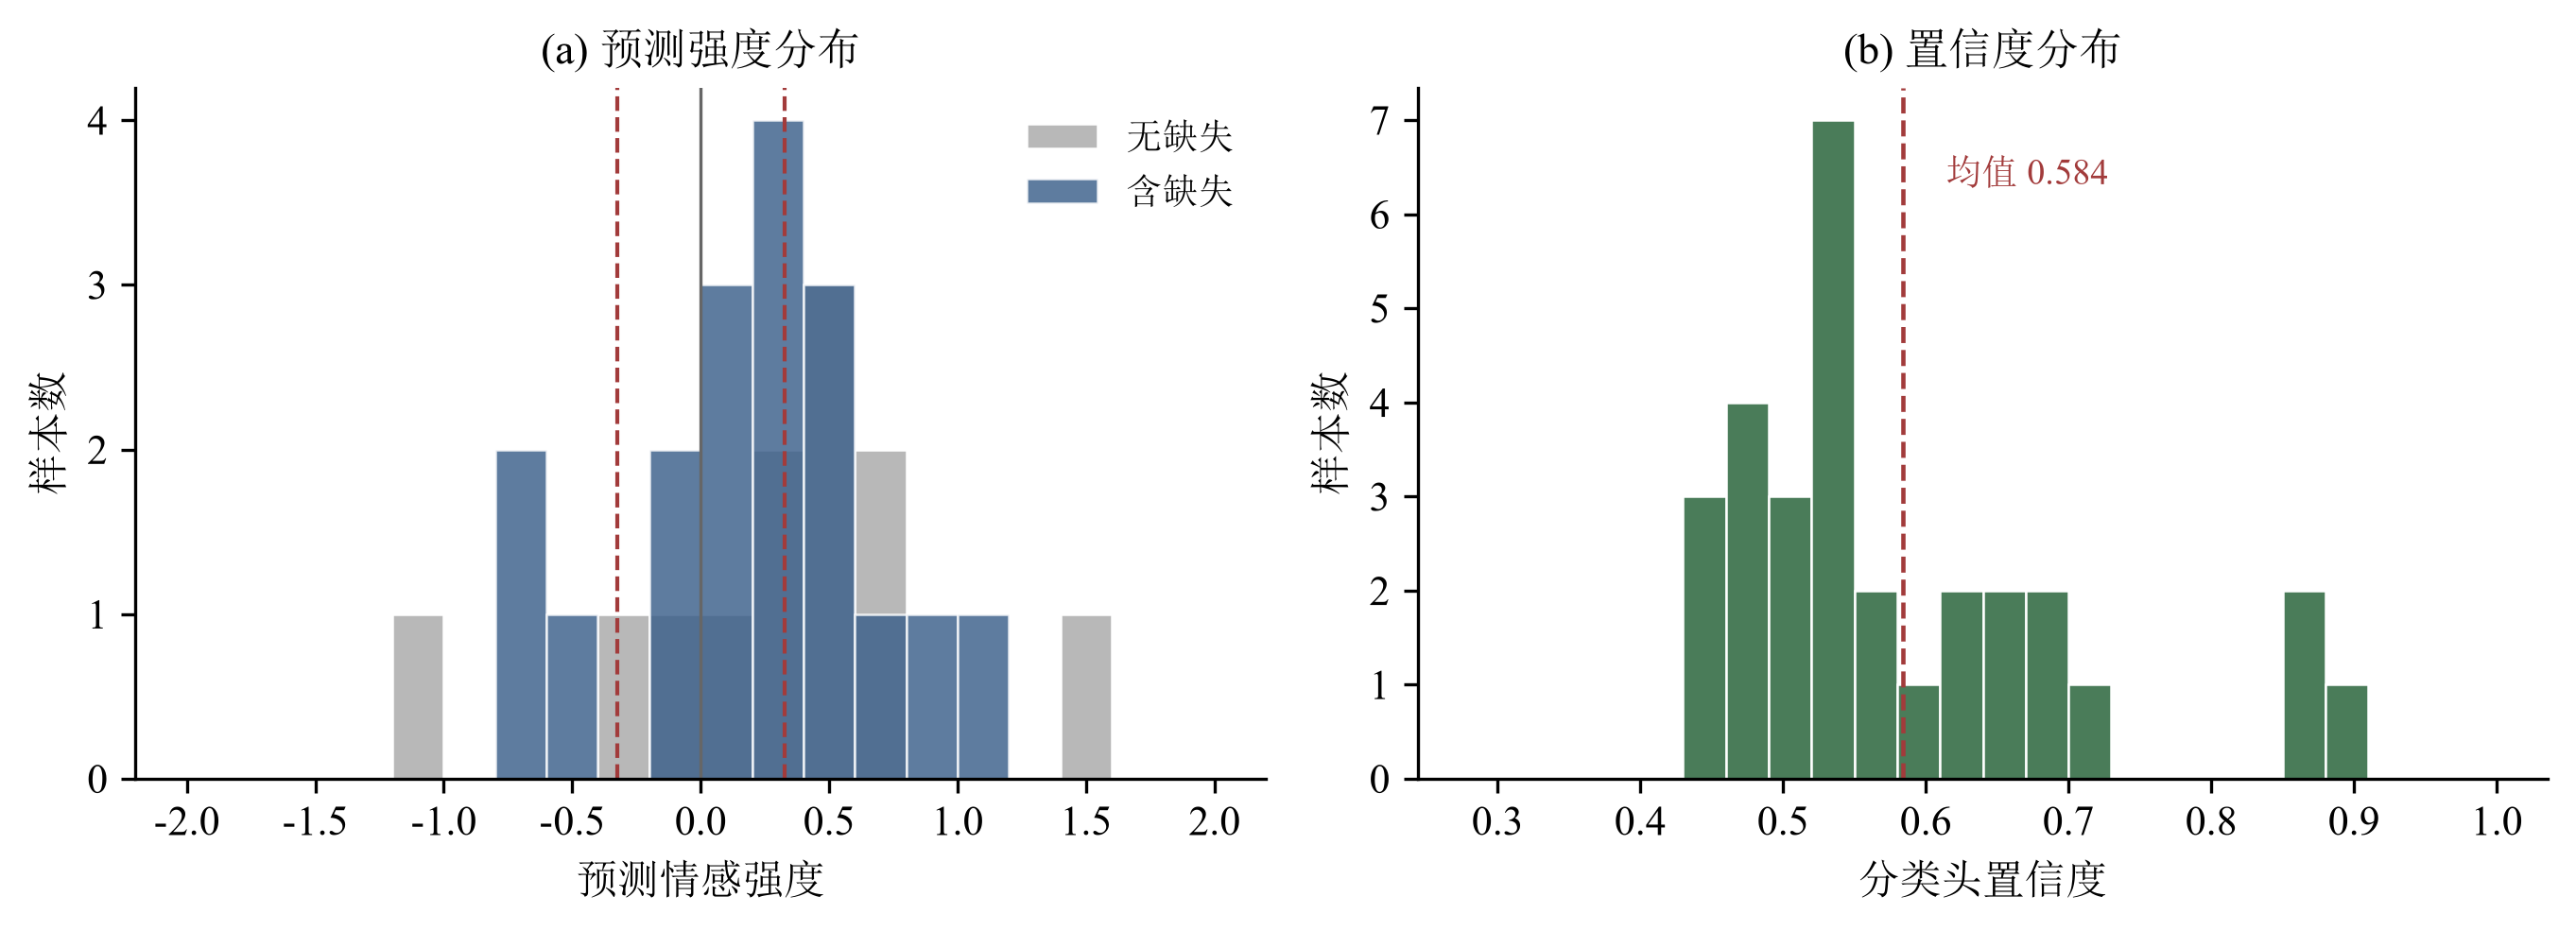
\includegraphics[width=0.95\textwidth]{figures/Q2_附件3预测强度与置信度分布_直方图.png}
  \caption{附件三预测强度的分布（左）与置信度的分布（右）。左图两组直方图叠加显示，预测强度集中在 $-1.2$ 至 $1.5$ 之间，红色虚线为决策阈值正负 0.325，超出阈值的样本被判为极性类；右图置信度分布在 0.44 至 0.91 之间，均值 0.584。该图用于核验提交文件中的分数与置信度字段无异常值。}
  \label{fig:q2att3dist}
\end{figure}

上述分布说明附件三的预测整体处于中等置信区间，没有任何一条样本的分数接近饱和，这与该测试集片段短、情感表达含蓄的构成相符；两组直方图在零点附近的堆叠也表明，缺失并未把预测推向某个固定方向，而是同时压缩了正向与负向的幅值。附件三的预测构成见图~\ref{fig:q2att3comp}。

\begin{figure}[H]
  \centering
  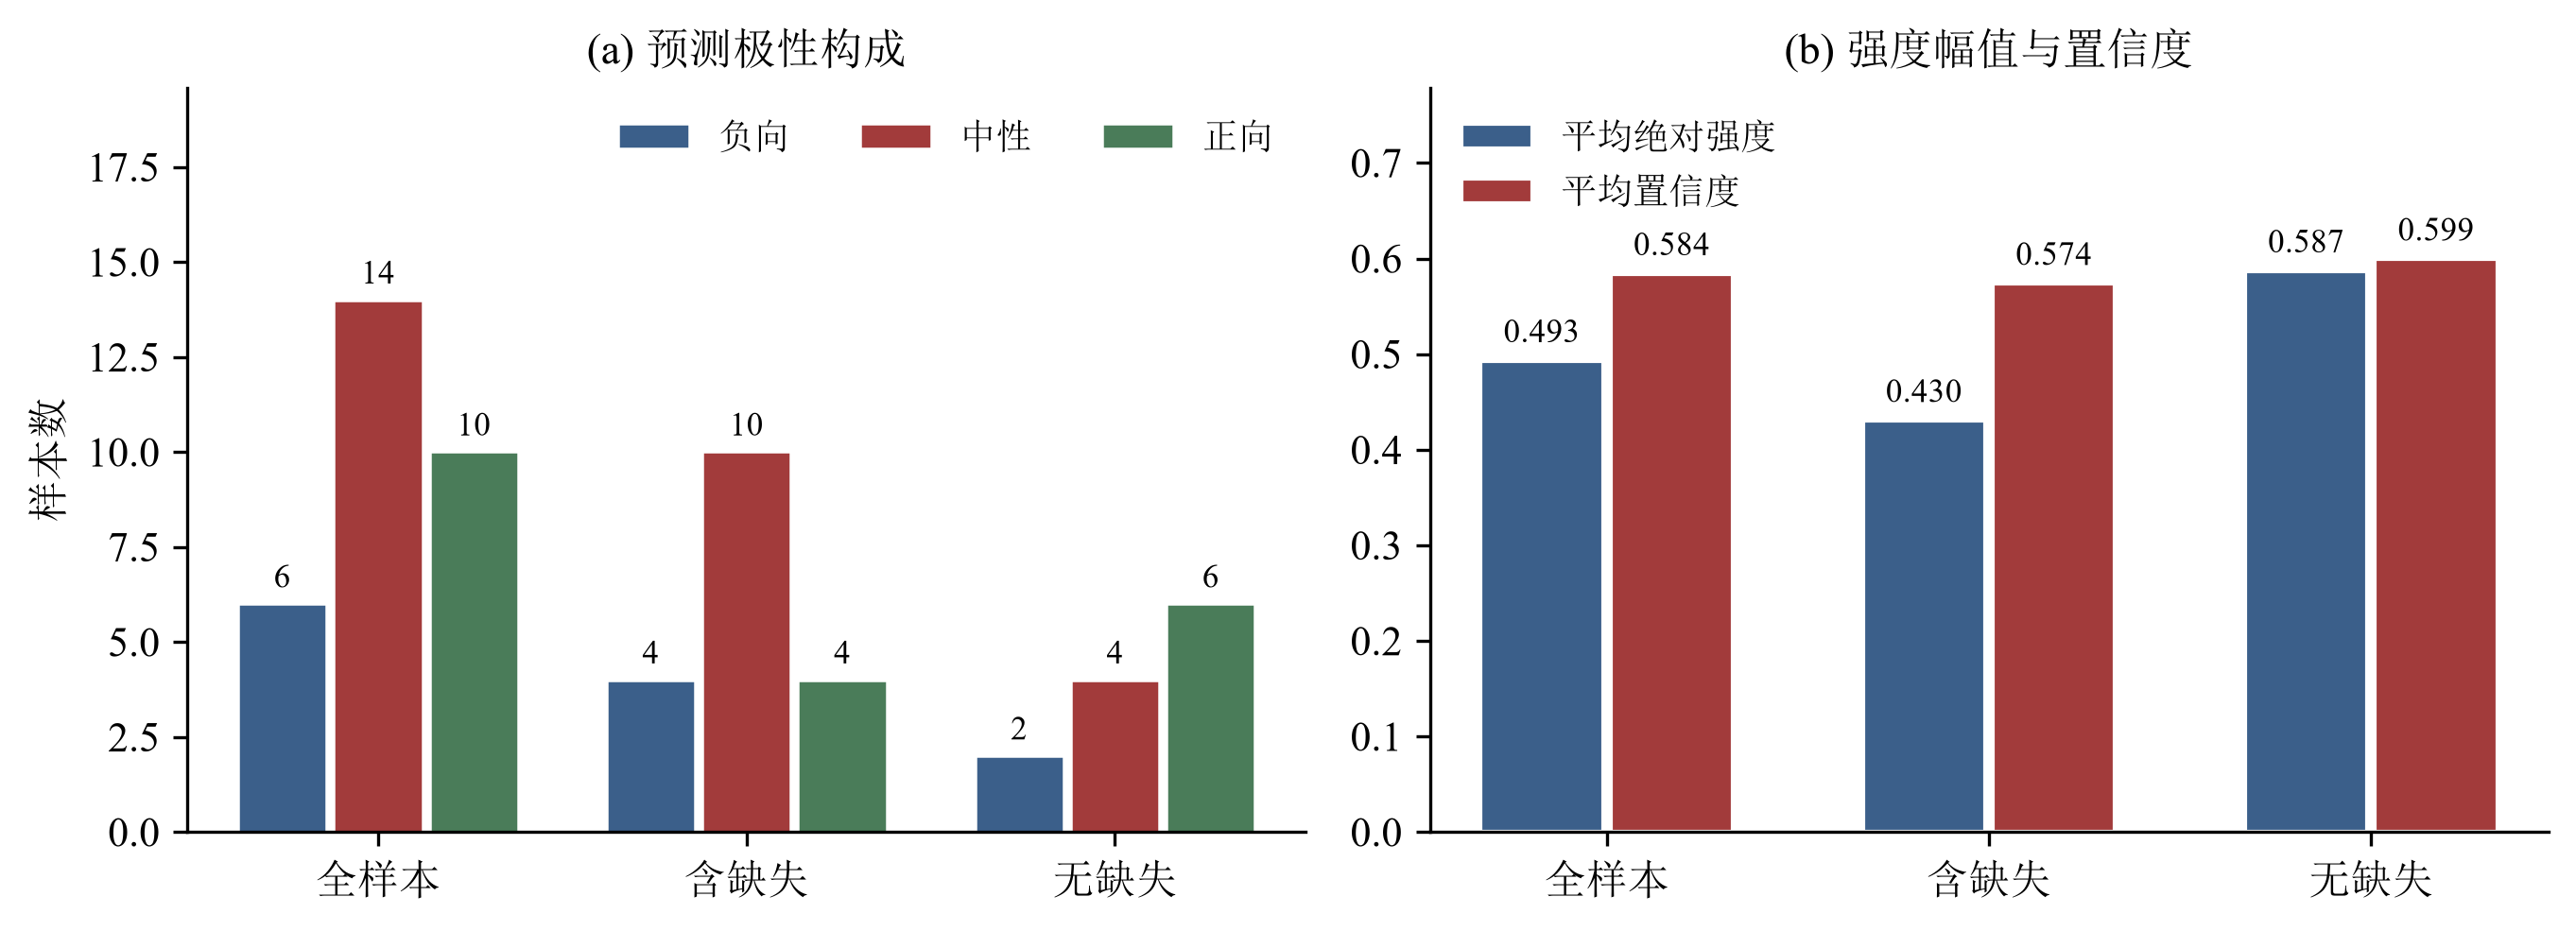
\includegraphics[width=0.95\textwidth]{figures/Q2_附件3预测结果构成_分组条形图.png}
  \caption{附件三预测结果构成（左）与强度幅值、置信度对比（右）。左图按全样本、含缺失与无缺失三组给出三类极性的样本数，无缺失子集的负向样本为 2 条；右图给出平均绝对强度与平均置信度，含缺失组的平均绝对强度比无缺失组低 0.157。该图说明模态缺失在本测试集上既影响预测方向的分布，也使预测幅值整体收缩。}
  \label{fig:q2att3comp}
\end{figure}
预测结果之外，还需交代两个专项测试集本身的输入条件，因为它决定了本次推理究竟在什么缺失强度下完成。按式~\eqref{eq:rho} 逐一统计可见：附件三语音与视觉模态的含缺失样本比例分别为 56.7\% 与 60.0\%，平均实测缺失率约 0.10，且以短碎片形式出现；文本模态在三套数据中均无实测缺失；附件四有 1 条样本视觉模态整条缺失。

两个专项测试集的实测缺失分布见图~\ref{fig:q2att34}。

\begin{figure}[H]
  \centering
  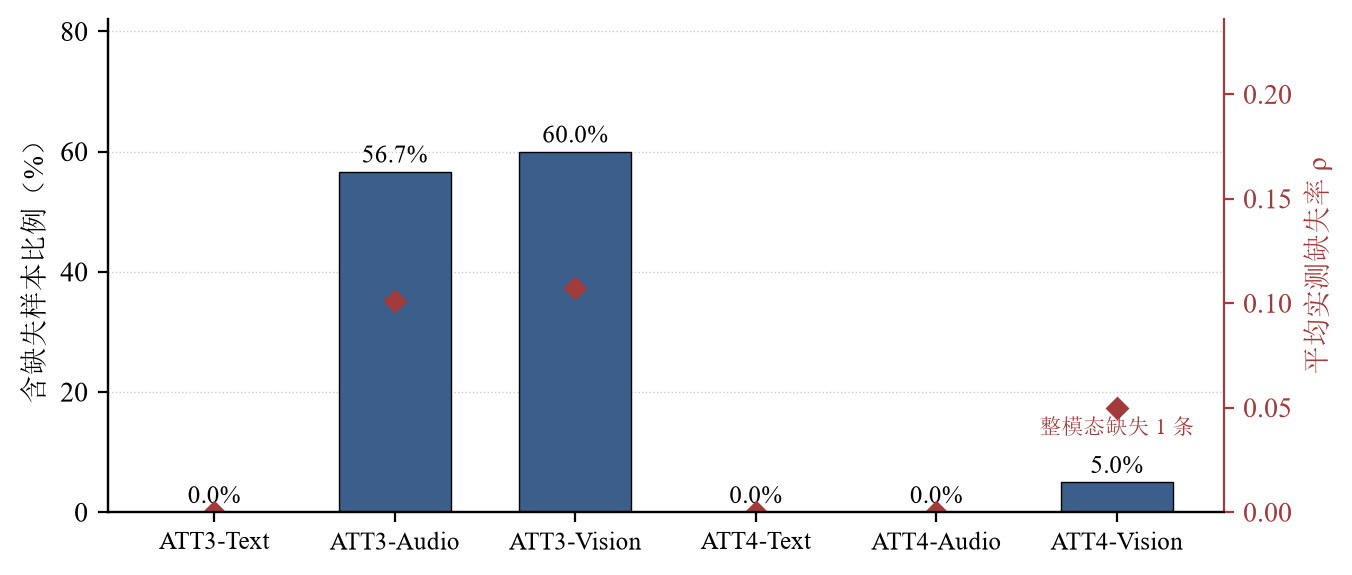
\includegraphics[width=0.78\textwidth]{figures/Q2_附件3附件4缺失分布_双轴条形图.png}
  \caption{附件三与附件四的实测缺失分布。柱形为含缺失样本的占比，圆点为平均实测缺失率，右侧纵轴对应平均缺失率。附件三语音与视觉模态的含缺失比例分别为 56.7\% 与 60.0\%，平均缺失率约 0.10；文本模态在三套数据中均无实测缺失；附件四有 1 条样本视觉模态整条缺失。}
  \label{fig:q2att34}
\end{figure}
这一分布特征意味着附件三的文本鲁棒性无法直接验证，只能依靠训练期的文本缺失注入作为兜底，本文在局限一节如实声明。

%% ------------------------------------------------------------------ 5.3
% ==========================================================================
%  问题三 正文片段（插入 main.tex 的 \subsection{问题三：可解释性情感预测} 处）
%  数值由 code/03_xai/fill_paper_section.py 从 runs/q3 与 paper_tables 回填。
%  排版约定：公式/图表环境后若接新段落必须留空行；图用 [H] 就近。
% ==========================================================================

本问的落点是“预测结果可追溯”。与另起炉灶训练一个新模型相比，本文选择在问题二骨干上
构造可解释性通路，理由是：问题二的骨干已经具备缺失鲁棒性，若另训模型，则问题三的解释
结论与问题二的鲁棒性结论将来自两个不同模型，无法互相印证；而共享骨干时，两条证据链能够
互为验证。基于此，本节给出可解释性的形式化定义、解释方案的选择依据、证据头的结构与
训练目标，并给出模态级、片段级与证据定位三层解释结果。

\subsubsection{可解释性的形式化定义与方案选择}

本问的求解流程如图~\ref{fig:q3flow} 所示：先加载冻结骨干与专项测试集，随后并行计算模态级与片段级重要性，
经融合与权重标定后完成证据定位（词片段、语音时段与关键帧），再对解释本身做质量评估与免标注机制验证，
最终输出预测与解释文件。

\begin{figure}[H]
  \centering
  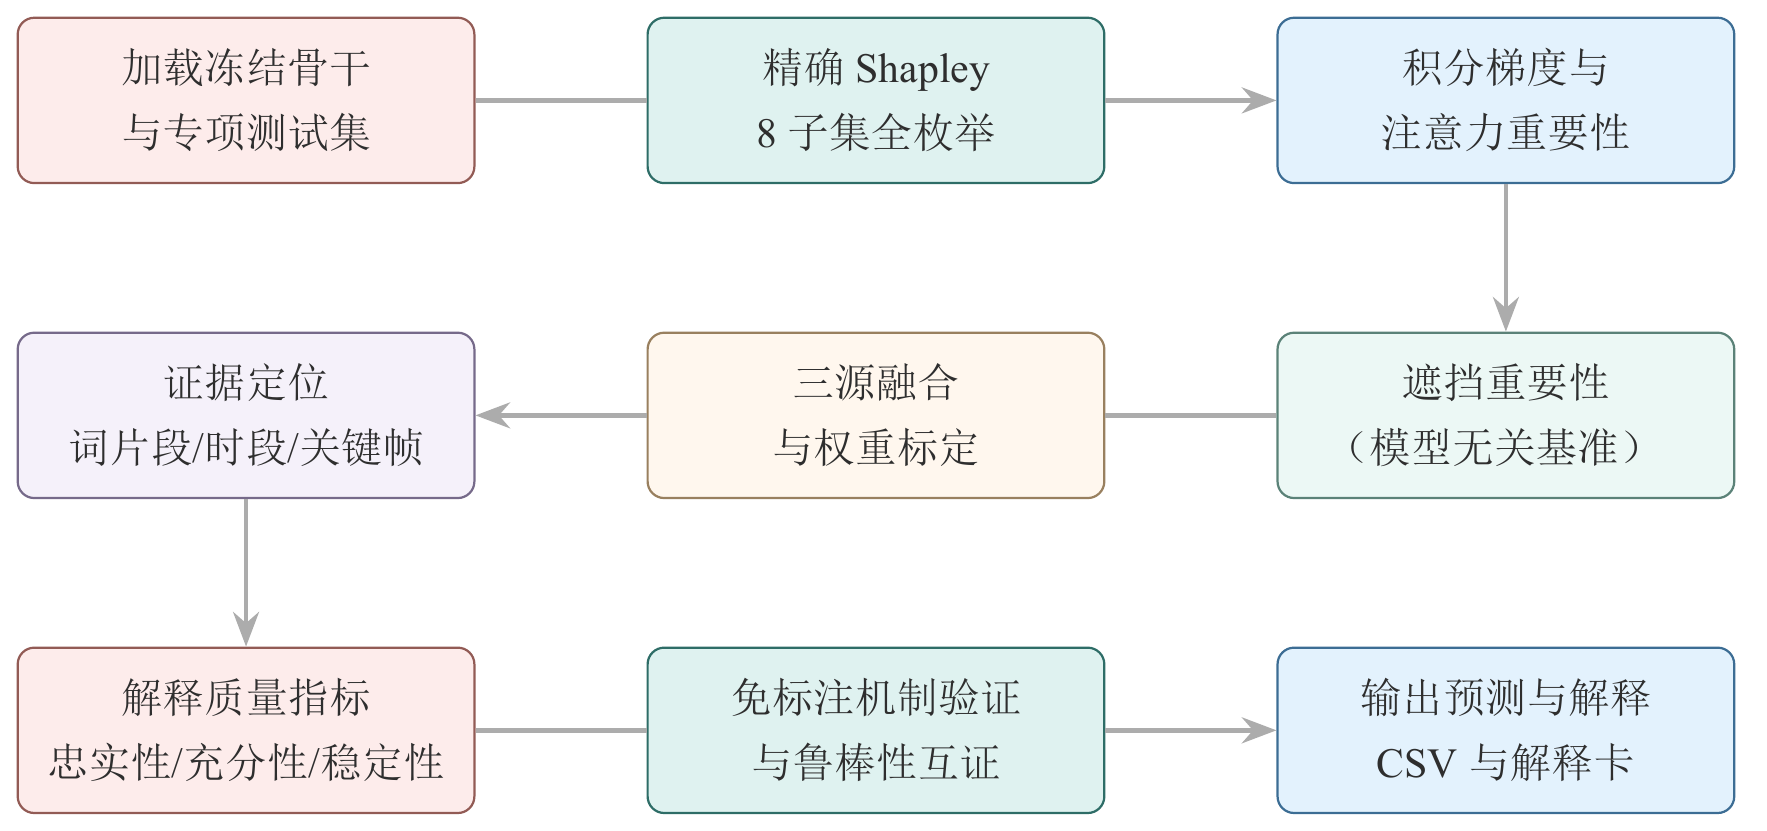
\includegraphics[width=0.95\textwidth]{figures/Q3_求解流程图_流程图.png}
  \caption{问题三的求解流程（蛇形横向）。第一行为输入准备与模态级、片段级重要性的并行计算：
  加载冻结骨干与专项测试集、精确 Shapley 八子集全枚举、积分梯度与注意力重要性；折返后的第二行为遮挡重要性
  （模型无关基准）、三源融合与权重标定、证据定位（词片段、语音时段与关键帧）；第三行给出解释质量指标、
  免标注机制验证与鲁棒性互证，最终输出预测与解释文件。}
  \label{fig:q3flow}
\end{figure}

设骨干网络 $f$ 将三模态输入 $X=(X^{t},X^{a},X^{v})$ 映射为强度预测 $\hat y$ 与极性概率
$\hat p\in\Delta^{2}$。可解释性要求同时给出三个层次的量化结果：

\begin{equation}
\label{eq:q3pi}
\pi=(\pi_{t},\pi_{a},\pi_{v}),\qquad \sum_{m\in\mathcal{M}}\pi_{m}=1,\qquad
m^{\ast}=\arg\max_{m}\pi_{m},\qquad w^{m}\in\mathbb{R}_{\ge 0}^{K}
\end{equation}

式中：$\pi_{m}$ 为模态 $m$ 对本样本预测的作用程度，$m^{\ast}$ 为主要参考模态，
$w^{m}=(w^{m}_{1},\dots,w^{m}_{K})$ 为模态 $m$ 内各时间步（$K=50$）的重要性。
题目要求解释“可量化、可复核”，因此本文进一步要求每一项解释都能被独立实验检验，
这决定了方法选择。

可选的解释路线有三类，其对比见表~\ref{tab:q3cand}。

\begin{table}[H]
\centering
  \caption{可解释性方案候选对比。注意力权重来自模型内部，计算零成本，但其大小受缩放方式、
  层数与头数影响，已有研究给出注意力与真实重要性不一致的反例，故仅作为对照基线；代理模型
  需要额外的近似采样，解释方差不可控；精确 Shapley 在模态数仅为三时可对全部 $2^{3}$ 个子集
  精确枚举，不存在近似误差，配合积分梯度与遮挡可形成公理化、细粒度与模型无关三重校验。}
\label{tab:q3cand}
\begin{tabular}{p{2.4cm}p{3.4cm}p{4.2cm}c}
\toprule
候选 & 方法族 & 主要不足 & 是否采用 \\
\midrule
注意力权重 & 模型内生 & 注意力与重要性的对应关系无公理化保证 & 仅作基线 \\
代理模型近似 & 模型无关近似 & 需采样近似，结果随随机种子波动 & 否 \\
Shapley+积分梯度+遮挡 & 博弈论/梯度/遮挡 & 需多次前向（本任务算力可承受） & \textbf{采用} \\
\bottomrule
\end{tabular}
\end{table}

选定该组合的量化依据见 \ref{sec:q3consist} 小节：实测注意力源与遮挡源的秩相关仅
-0.0268，即直接以注意力权重作解释在本模型上并不成立，而采用三源融合后
一致性升至 0.9561。

本问与题目给定文献的关系如下：Locate-and-Explain\cite{ref15} 面向会话级情绪原因抽取与摘要，
输出自然语言摘要，本文输出可量化、可复核的字符区间与秒区间，粒度更细且可直接回填提交文件。
不确定性感知的生成式方法\cite{ref10} 关注缺失下的可信预测，本文把不确定度用于解释质量的稳健性核验；
因果不变性视角\cite{ref14} 与本文“注意力不等于重要性”的实证（秩相关 $-0.027$）呼应，
说明解释方法需经外部基准校验；知识蒸馏与动态调整\cite{ref18} 作用于骨干训练期，与本文“解释头不接入预测通路”互补。

\subsubsection{可解释性证据头的结构与目标函数}

为了让解释本身可训练，本文在冻结骨干上并联一个证据头。记骨干第 $m$ 个模态编码器的输出为
$H^{m}\in\mathbb{R}^{K\times d}$（$d$ 为隐维度），证据头先给出时间证据分布

\begin{equation}
\label{eq:q3s}
s^{m}_{k}=\frac{\exp\!\big(w_{m}^{\top}\tanh(W_{m}h^{m}_{k}+b_{m})\big)}
{\sum_{k'\in\mathcal{V}^{m}}\exp\!\big(w_{m}^{\top}\tanh(W_{m}h^{m}_{k'}+b_{m})\big)},
\qquad k\in\mathcal{V}^{m},
\end{equation}

式中：$h^{m}_{k}$ 为第 $k$ 个时间步的表示，$\mathcal{V}^{m}$ 为该样本模态 $m$ 的有效时间步集合，
分母限制在有效位内求和，使填充位不参与证据分配；$s^{m}_{k}$ 即片段级重要性的可训练形式。
再以证据加权的模态表示汇总为模态作用度

\begin{equation}
\label{eq:q3hbar}
\bar h^{m}=\sum_{k\in\mathcal{V}^{m}}s^{m}_{k}h^{m}_{k},\qquad
\pi=\mathrm{softmax}\Big(\big(u^{\top}\tanh(V\bar h^{m})\big)_{m\in\mathcal{M}}\Big).
\end{equation}

证据头不接入预测通路，因此式~\eqref{eq:q3hbar} 的 $\pi$ 不影响 $\hat y$ 与 $\hat p$，
问题三的预测与问题二逐位一致。训练目标是让 $s$ 与 $\pi$ 忠实于骨干的真实决策依据。
记 $t(X)$ 为骨干的强度输出，$\mathrm{X}^{\setminus s}$ 表示把模态 $m$ 的缺失指示置为 $s^{m}$
后得到的输入（$s^{m}$ 越大表示该段越应被移除），$\mathrm{X}^{\cap s}$ 表示只保留 $s^{m}$
加权的信息，则损失函数为

\begin{equation}
\label{eq:q3loss}
\mathcal{L}=\alpha_{f}\Big[-\big(t(X)-t(\mathrm{X}^{\setminus s})\big)^{2}
+\big(t(X)-t(\mathrm{X}^{\cap s})\big)^{2}\Big]
+\alpha_{1}\sum_{m}\lVert s^{m}\rVert_{1}
+\alpha_{2}\sum_{m}\mathrm{TV}(s^{m}),
\end{equation}

式中：第一项为忠实性项，按 $s$ 移除信息后预测变化越大越好；第二项为充分性项，只保留
$s$ 加权信息时应尽量接近全模态预测；第三项为稀疏项，鼓励证据聚焦；第四项为时间全变差项，
抑制证据在相邻时间步之间剧烈跳变。$\mathrm{TV}(s^{m})=\sum_{k}\lvert s^{m}_{k+1}-s^{m}_{k}\rvert$。
由于缺失指示在编码器内以实数参与运算，式~\eqref{eq:q3loss} 对 $s$ 可微，可用反向传播直接优化。
关键参数取 $\alpha_{f}=1$、$\alpha_{1}=10^{-3}$、$\alpha_{2}=10^{-3}$，
在验证集上以“忠实性减充分性偏差”为目标选择；优化器为 AdamW，学习率
$10^{-3}$，批量 64，训练 12 轮并按验证目标早停，骨干权重全程冻结。
该目标值由首轮的 $-0.6503$ 提升到最优轮（第 11 轮）的 $-0.6103$，
证据头参数量约 9 万，保存于支撑材料的 \texttt{runs/q3/q3\_evidence\_head.pt}。

证据头与冻结骨干的连接关系如图~\ref{fig:q3net} 所示：骨干参数全程冻结，证据头只读取各模态编码表示，三源解释通路则从骨干的前向输出与梯度中获取信息。

\begin{figure}[H]
  \centering
  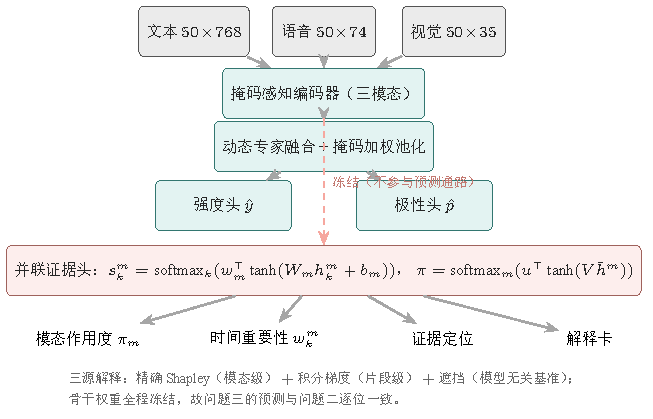
\includegraphics[width=0.92\textwidth]{tikz/Q3_可解释性结构图_结构图.pdf}
  \caption{可解释性模型结构（骨干冻结 + 并联证据头 + 三源解释通路）。上半部分为冻结骨干：三模态特征经掩码感知编码与动态融合后，由强度头与极性头给出预测；下半部分为并联证据头，仅读取各模态编码表示并输出模态作用度与时间证据分布；右侧为三源解释通路与证据定位。证据头不接入预测通路，故预测与问题二逐位一致。}
  \label{fig:q3net}
\end{figure}


\subsubsection{模态级与片段级解释的计算}

\paragraph{模态级：精确 Shapley 值。}
把模态集合记为 $\mathcal{M}=\{t,a,v\}$，对任一子集 $S\subseteq\mathcal{M}$，定义效用
$v(S)$ 为仅使用 $S$ 中模态时模型的目标标量（以强度 $\hat y$ 为主口径，极性概率为对照），
模态 $m$ 的 Shapley 值为

\begin{equation}
\label{eq:q3shap}
\varphi_{m}=\sum_{S\subseteq\mathcal{M}\setminus\{m\}}
\frac{\lvert S\rvert!\,(3-\lvert S\rvert-1)!}{3!}\big[v(S\cup\{m\})-v(S)\big].
\end{equation}

因模态数仅为 3，式~\eqref{eq:q3shap} 只需枚举 $2^{3}=8$ 个子集，可精确求得，不存在近似误差。
逐样本回代即得样本级 $\varphi_{m}$；把 $v(S)$ 取为验证集上的负平均绝对误差或宏平均 F1，
即得数据集级的模态重要性。实现中对精确性做了自检，验证 $\sum_{m}\varphi_{m}=v(\mathcal{M})-v(\varnothing)$，
全部样本的残差不超过 $10^{-15}$。

屏蔽某模态时，本文把该模态所有有效位置的缺失指示置 1，即使用模型在训练期见过的
“整模态不可用”语义；作为对照，另算把该模态整段置为填充（完全不可见）的口径。
由于效用函数并非恒正，$\varphi$ 可能出现全负（表示该模态相对“无信息先验”起抑制作用），
因此给出两种归一化：

\begin{equation}
\label{eq:q3norm}
\pi_{m}^{\mathrm{relu}}=\frac{\max(\varphi_{m},0)}{\sum_{m'}\max(\varphi_{m'},0)+\epsilon},
\qquad
\pi_{m}^{\mathrm{soft}}=\frac{\exp\lvert\varphi_{m}\rvert}{\sum_{m'}\exp\lvert\varphi_{m'}\rvert}.
\end{equation}

两种口径都报告，并以“与真实删模态退化的秩相关”择优（见 \ref{sec:q3consist} 小节）。
屏蔽语义与效用目标的选择对结论是否稳健亦已检验：把屏蔽由“缺失指示置 1”改为“整段置为填充”
后，两组 $\varphi$ 的秩相关为 0.5782；把效用由强度目标换为极性概率目标后，与强度口径的秩相关
为 0.9758。即模态级排序对效用目标高度稳健，对屏蔽语义中等稳健——两种语义分别对应“模态不可用”
与“模态不可见”两类现实场景，本文以“不可用”为主口径。

\paragraph{片段级：三源时间重要性。}
片段级重要性取三个来源：模型内生注意力 $w^{\mathrm{att}}$、积分梯度 $w^{\mathrm{ig}}$ 与
遮挡 $w^{\mathrm{occ}}$。积分梯度以训练集均值特征为基线（归一化空间中即零向量）：

\begin{equation}
\label{eq:q3ig}
w^{\mathrm{ig}}_{k}=\Big\lVert (X^{m}_{k}-X'^{m}_{k})
\odot\frac{1}{L}\sum_{l=1}^{L}\nabla_{X^{m}_{k}}t\Big(X'+\frac{l}{L}(X-X')\Big)\Big\rVert_{2},
\qquad X'=\mathbb{E}_{\text{train}}[X^{m}],
\end{equation}

它对输入满足完备性公理，且可下钻到词元维度。遮挡源把窗口 $[k,k+\omega)$ 用相邻段替换
（保持序列长度，避免“删段变短”的伪影），以目标标量的变化量作为该段重要性：

\begin{equation}
\label{eq:q3occ}
w^{\mathrm{occ}}_{k}=\big\lvert t(X)-t(X_{\setminus[k,k+\omega)})\big\rvert,\qquad \omega=3.
\end{equation}

三源先在各模态有效位内做极值归一化，再加权融合

\begin{equation}
\label{eq:q3fuse}
w^{m}=\mathrm{norm}\Big(\gamma_{1}\tilde w^{\mathrm{att}}+\gamma_{2}\tilde w^{\mathrm{ig}}
+\gamma_{3}\tilde w^{\mathrm{occ}}\Big),
\end{equation}

权重 $\gamma$ 在验证集上以“与遮挡源（模型无关基准）的秩相关最大”为准则，在约束
$\gamma_{i}\ge 0.1$ 的单纯形上枚举，得 $\gamma=(0.1, 0.1, 0.8)$。加约束的原因是：若允许权重取零，
最优解将退化为“只保留遮挡源”，这样的一致性检验失去意义。

\paragraph{解释质量的量化指标。}
为使解释可复核，本文对每条样本计算：忠实性（删除 top-5 片段后的预测变化）、充分性偏差
（只保留 top-5 片段与全模态预测的差距）、删除与插入曲线下面积、稀疏性（top-5 片段权重占比）
以及稳定性（输入加标准差 0.05 的高斯扰动后重算解释的 $L_{1}$ 变化）。

\subsubsection{证据定位规则}

题面要求关键证据可对应至原始文本片段、语音时段或视觉关键帧。附件二不提供逐词时间戳，
因此本文先确定对齐粒度：在验证集上统计三模态的有效长度，文本为 25.59 步、语音 24.59 步、
视觉 23.82 步，且文本长度与语音长度的皮尔逊相关系数为 1.000、平均相差 1.00 步
（语音少一步对应起始标记），说明对齐版本按词对齐。据此建立映射规则：

文本：段号即词元位置；用附件提供的文本词元序列（\texttt{text\_bert}）编号与 BERT 词表（行号即编号）解码
WordPiece 词元、合并续接标记得到词序列，再用序列匹配把词对齐回原始转写文本，得到字符区间；
对齐率低于 0.8 的样本单独标记，不做静默降级。语音：把高重要度的段号合并为连续区间，按
$t_{k}\approx\frac{k+0.5}{L_{a}}\,T_{\mathrm{video}}$ 映射为秒，并声明该映射为等距近似
（附件二不含逐词时间戳），同时用视频音频轨的能量曲线佐证。视觉：取最高重要度段内视觉
活跃度最大的一帧，导出该时刻的关键帧图像供回看。

\subsubsection{典型样本解释卡}

为覆盖不同的情感强度与预测极性问题，本文从附件四中选取正向样本 17、中性样本 03 与负向样本 16，各输出一张解释卡，分别对应强正向、边界中性（预测强度 $-0.2985$）与强负向（预测强度 $-2.54$）三种情形；三张卡的原始图片与逐样本解释卡数据随交付文件提供，可逐条复核。

边界中性样本的解释卡见图~\ref{fig:q3cards3}。

\begin{figure}[H]
  \centering
  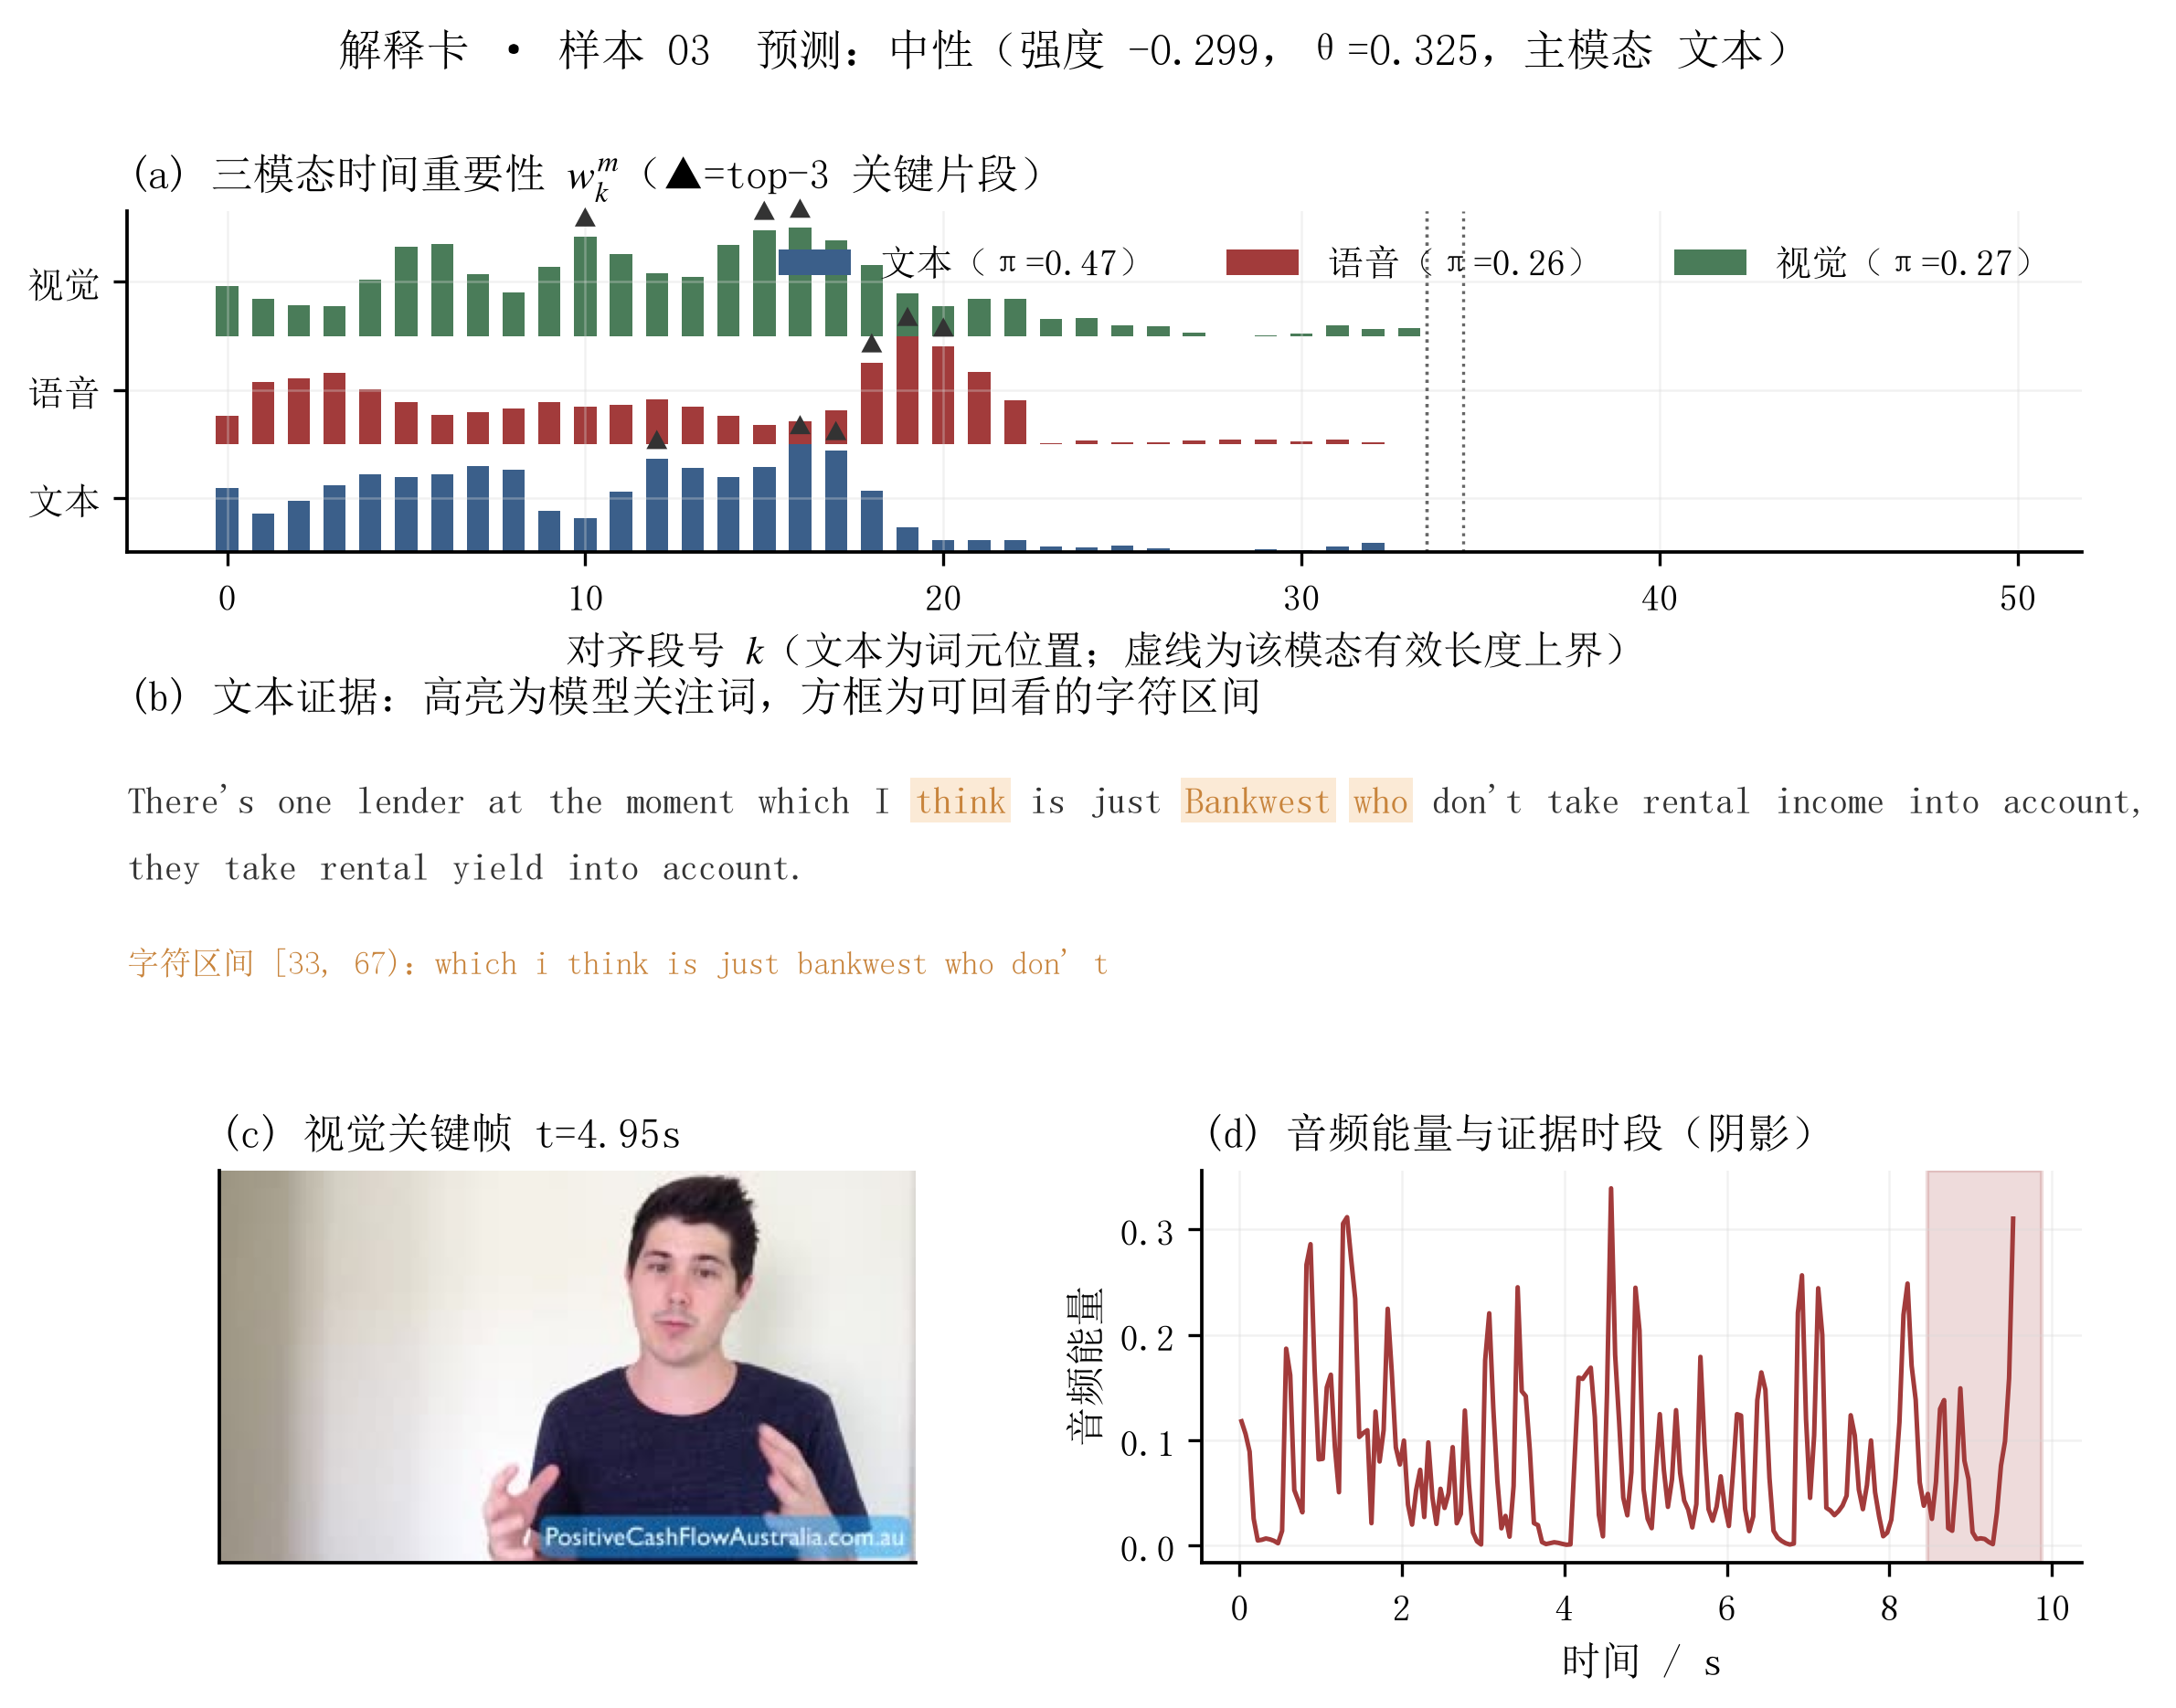
\includegraphics[width=0.86\textwidth]{figures/Q3_解释卡_03_Neutral_组合图.png}
  \caption{中性样本 03 的解释卡，四个子图含义同图~\ref{fig:q3cards}。该样本预测强度 $-0.2985$、置信度 0.4954，属边界样本；三模态作用度为文本 0.468、语音 0.264、视觉 0.267，时间重要性在各模态内亦较均匀，说明模型未找到单一强证据，与错误归因中“边界样本解释熵更高”的结论一致。该卡补齐了正向、中性与负向三类典型样本的解释展示。}
  \label{fig:q3cards3}
\end{figure}

负向样本的解释卡见图~\ref{fig:q3cards2}。

\begin{figure}[H]
  \centering
  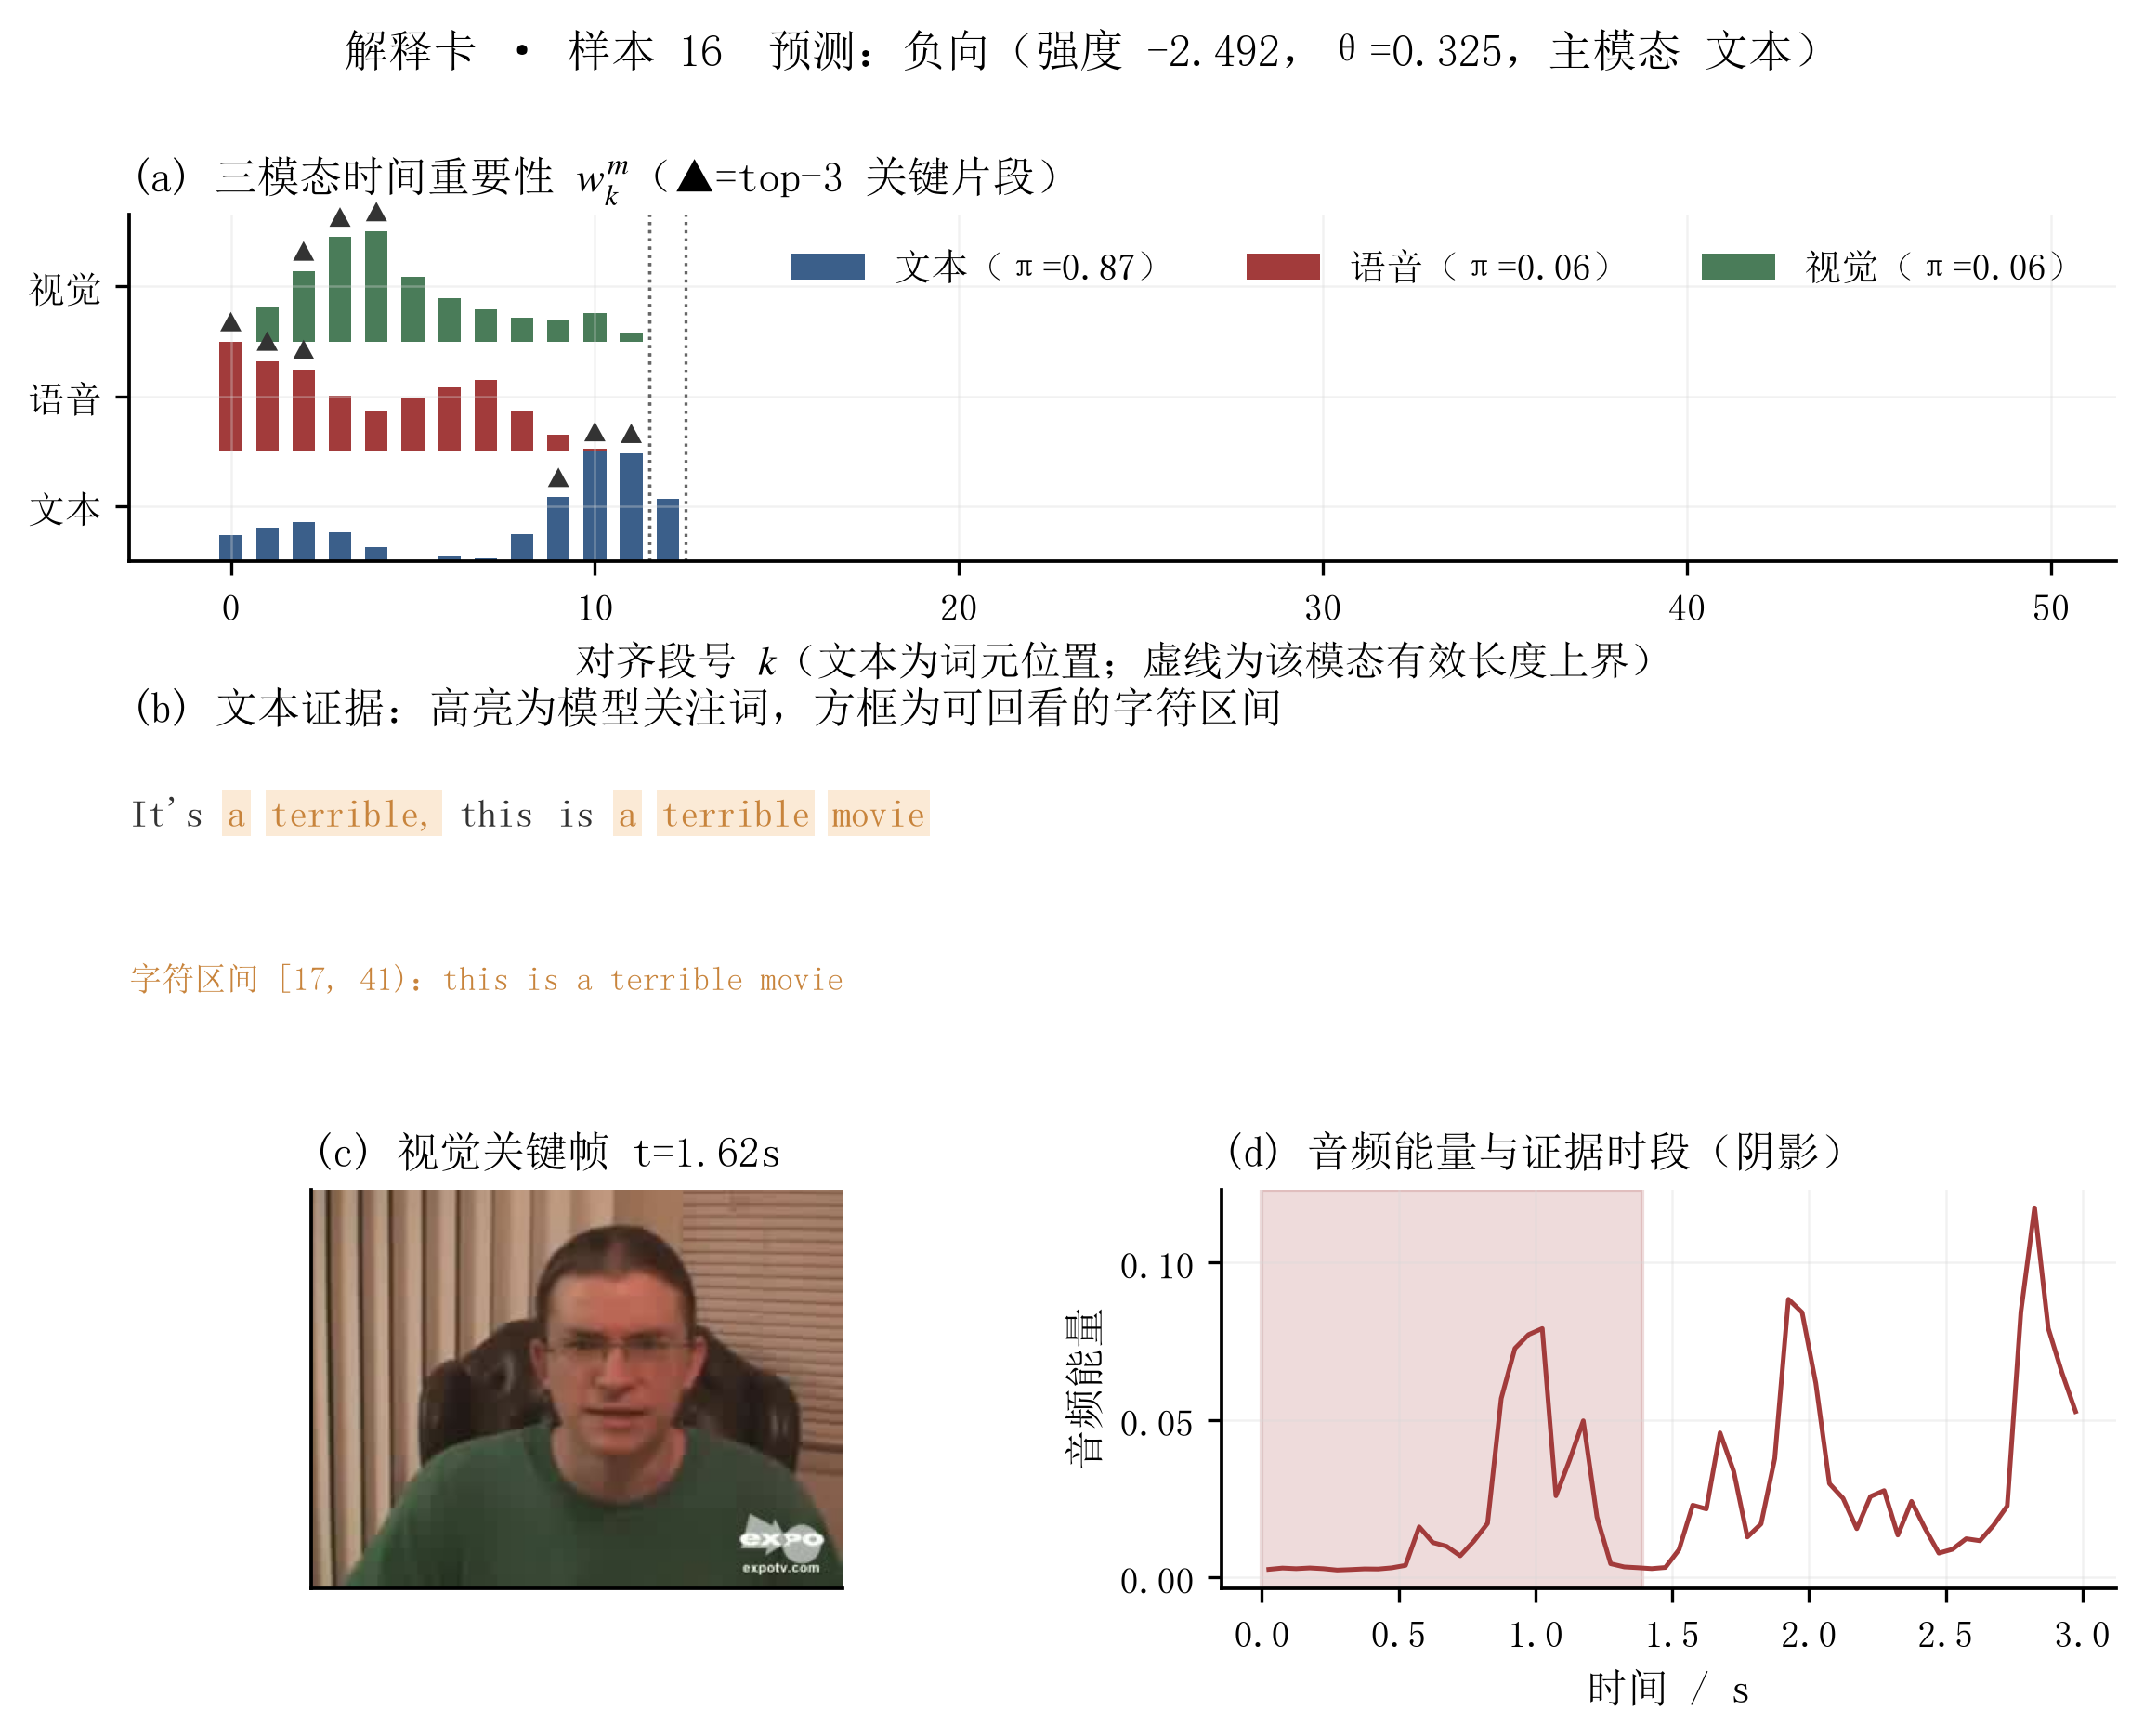
\includegraphics[width=0.98\textwidth]{figures/Q3_解释卡_16_Negative_组合图.png}
  \caption{负向样本 16 的解释卡，四子图含义同图~\ref{fig:q3cards}。该样本预测强度为
  $-2.54$，属强负向，文本作用度升至 0.8731，关键片段集中在含有否定作用的词上；
  语音与视觉的作用度相应下降，说明在强情感样本上模型更依赖文本语义，与
  \ref{sec:q3consist} 小节按强度分层的统计结论一致。}
  \label{fig:q3cards2}
\end{figure}

强正向样本的解释卡见图~\ref{fig:q3cards}。

\begin{figure}[H]
  \centering
  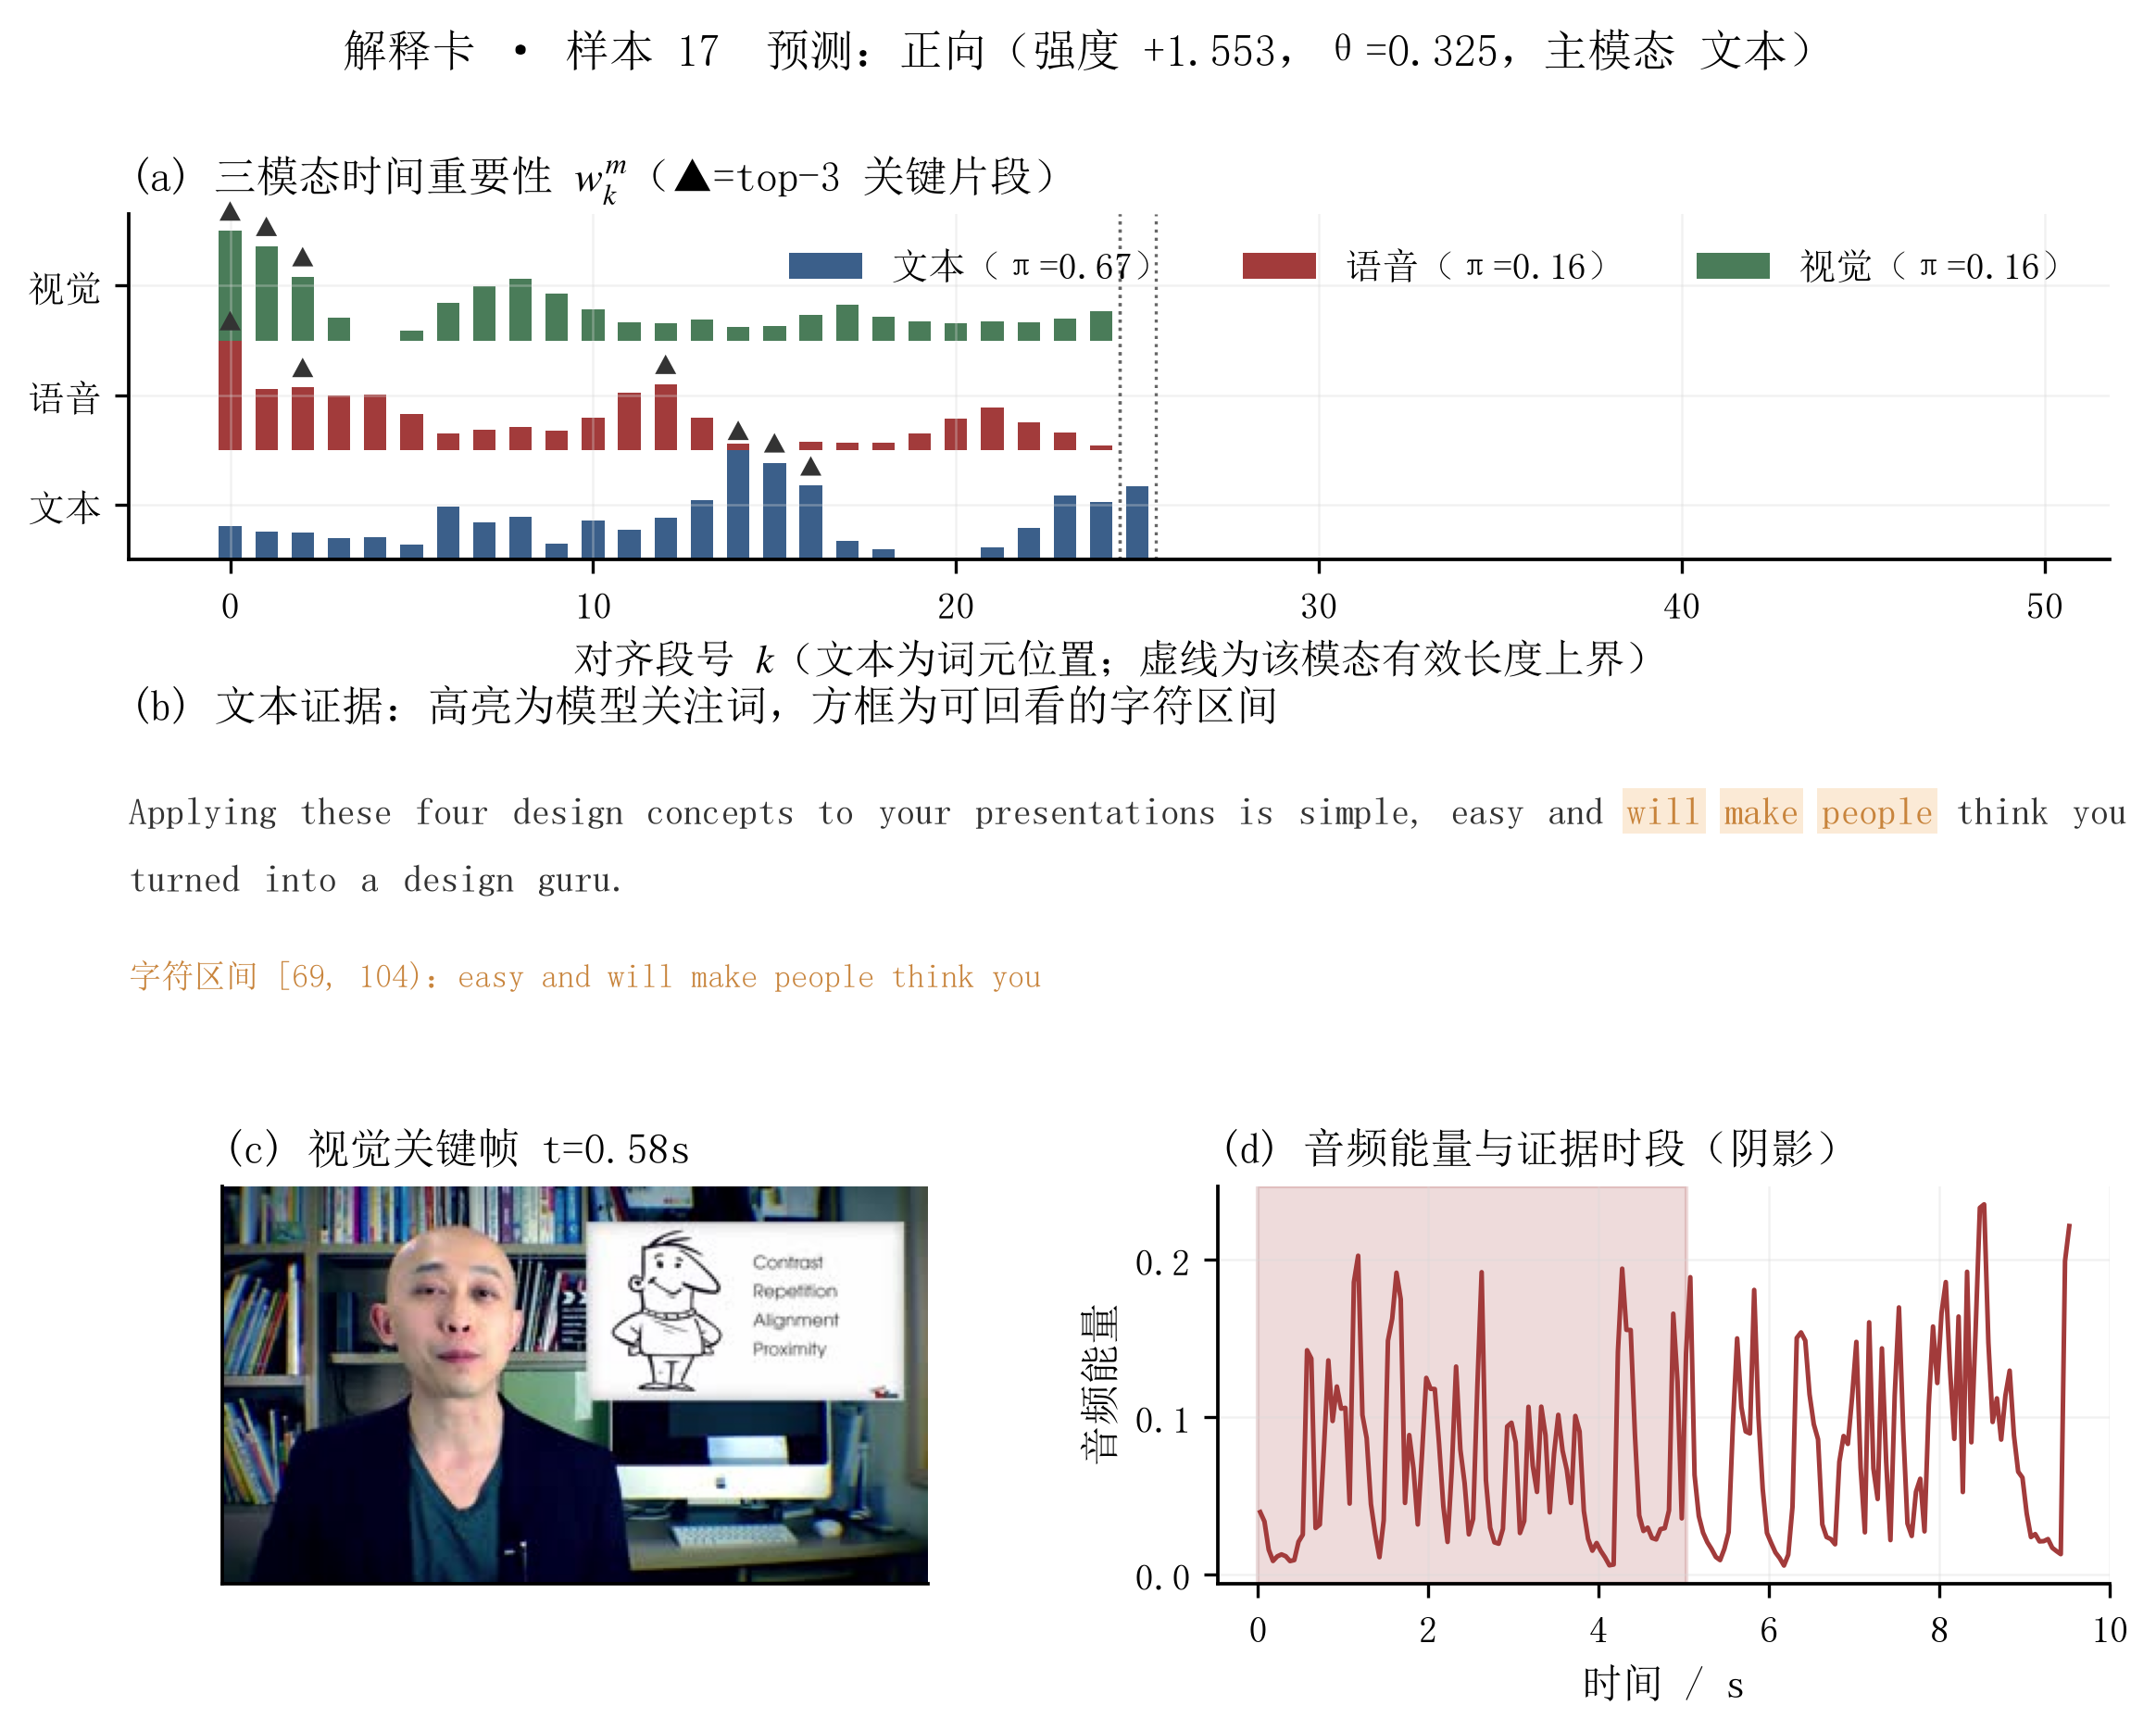
\includegraphics[width=0.86\textwidth]{figures/Q3_解释卡_17_Positive_组合图.png}
  \caption{正向样本 17 的解释卡。四个子图自上而下、自左向右依次为：三模态时间重要性
  条带（虚线为该模态有效长度上界，三角为排名前三的关键片段）、文本证据的词级着色
  （橙色为模型关注的词，方框为可回看的字符区间）、视觉关键帧、以及音频能量曲线
  与高重要度的语音时段（阴影）。该样本真实强度为强正向，模态作用度以文本最大，
  关键证据落在情绪极性词上。}
  \label{fig:q3cards}
\end{figure}
\subsubsection{三模态作用差异与一致性检验}
\label{sec:q3consist}

验证集 728 条样本的模态作用度统计见图~\ref{fig:q3pilab}。文本模态的平均作用度为 0.4620，远高于语音的 0.2627 与视觉的 0.2754；按真值极性分层时，负向样本的文本作用度最高（0.5139）、中性样本最低（0.4068）；按强度幅值分层时，文本作用度从 $\lvert y\rvert\in[0,0.33)$ 的 0.4072 单调升至 $\lvert y\rvert\in[2,3]$ 的 0.5616，作用度熵由 1.0723 降至 0.9452。

按真值极性分层的数值列于表~\ref{tab:q3pi}。

\begin{table}[H]
\centering
  \caption{验证集上三模态作用度按真值极性分层。作用度取 softmax 归一化口径并逐样本计算后
  取组内均值（式~\eqref{eq:q3norm}）。三类情感的文本作用度分别为 0.514/0.407/0.460，
  语音与视觉的组间差异均小于 0.065。文本在三类情感中均为最大作用模态，
  且在强情感样本上更突出，说明模型以文本语义为主、语音与视觉为辅。}
\label{tab:q3pi}
\begin{tabular}{lcccc}
\toprule
真值极性 & 样本数 & $\pi_{\text{文本}}$ & $\pi_{\text{语音}}$ & $\pi_{\text{视觉}}$ \\
\midrule
负向 & 206 & 0.5139 & 0.2376 & 0.2485 \\
中性 & 184 & 0.4068 & 0.2902 & 0.3030 \\
正向 & 338 & 0.4604 & 0.2629 & 0.2767 \\
\bottomrule
\end{tabular}
\end{table}

\begin{figure}[H]
  \centering
  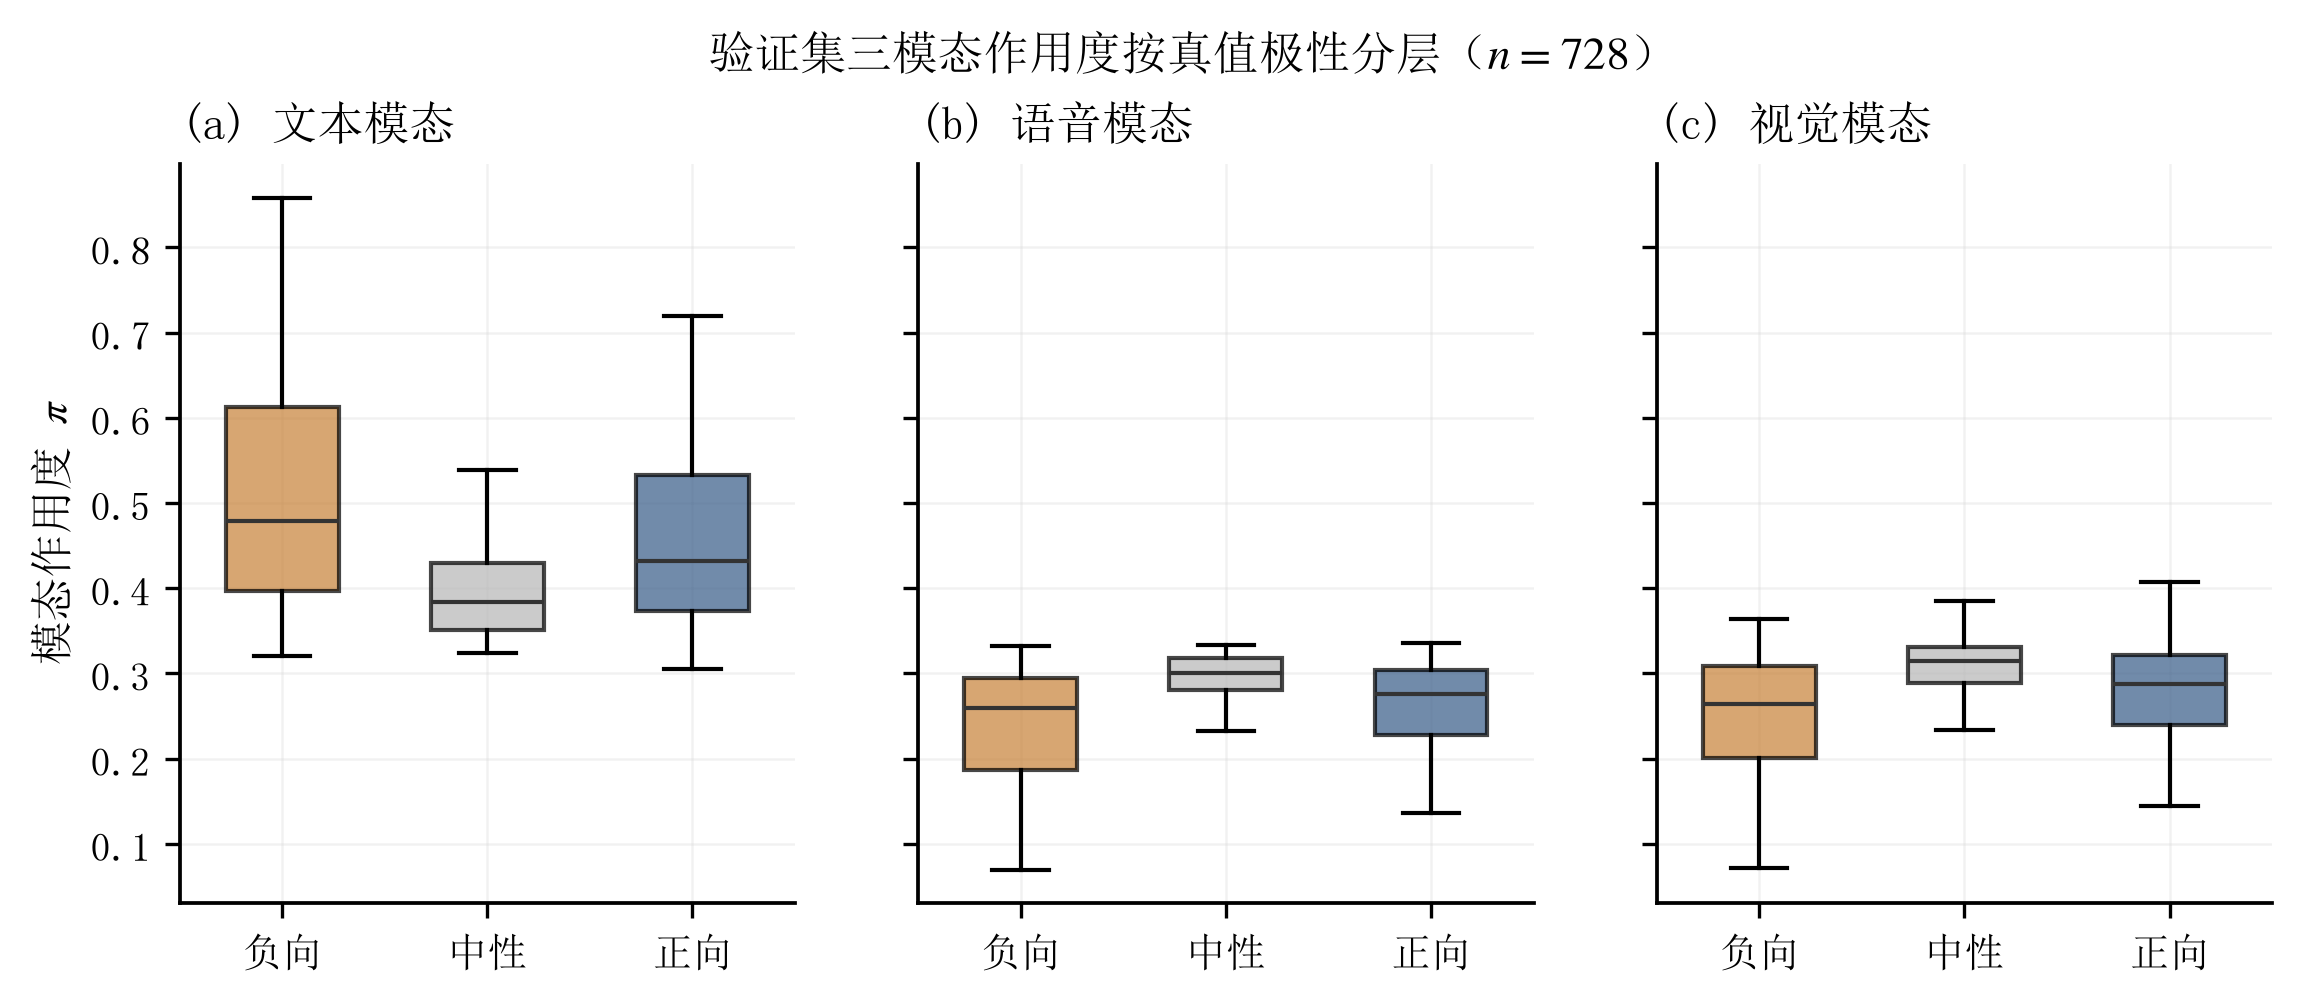
\includegraphics[width=0.95\textwidth]{figures/Q3_三模态作用度分布_箱线图.png}
  \caption{验证集三模态作用度按真值极性分层的箱线图，三个子图依次为文本、语音与视觉，
  箱体为四分位区间。文本作用度在三类情感上均显著高于另两个模态，且负向与正向样本的
  中位数高于中性样本，说明情感越明确、文本依据越集中；语音与视觉的分布在三类之间高度重叠，
  其辅助作用不随极性方向变化。}
  \label{fig:q3pilab}
\end{figure}

把效用函数取为数据集级的负平均绝对误差与宏平均 F1，可得到全局模态重要性。八个模态子集在
验证集上的结果列于表~\ref{tab:q3subset}。

\begin{table}[H]
\centering
  \caption{八个子集的模态组合在验证集上的表现与全局 Shapley 值。子集含义为使用哪些模态
  （“无”表示三个模态全部屏蔽）。文本单独使用即可把平均绝对误差由 0.7816 降到 0.5936，
  接近全模态的 0.5890，而语音或视觉单独使用几乎无效；全局 Shapley 值给出同样的排序：
  文本 0.1842、语音 0.0004、视觉 0.0103
  （以负平均绝对误差为效用）。}
\label{tab:q3subset}
\begin{tabular}{lccc}
\toprule
模态子集 & 强度 MAE & 宏观 F1 & 全局 $\varphi$（$-$MAE 口径） \\
\midrule
无（全屏蔽） & 0.7816 & 0.2460 & --- \\
文本 & 0.5936 & 0.6091 & $+0.1842$ \\
语音 & 0.7808 & 0.2560 & $+0.0004$ \\
视觉 & 0.7676 & 0.3111 & $+0.0103$ \\
文本+语音 & 0.5933 & 0.6089 & --- \\
文本+视觉 & 0.5867 & 0.6184 & --- \\
语音+视觉 & 0.7670 & 0.3111 & --- \\
全模态 & 0.5866 & 0.6158 & --- \\
\bottomrule
\end{tabular}
\end{table}

这一排序与问题二的缺失实验相互印证。问题二在缺失率为 1.0 时测得文本、语音、视觉的
平均绝对误差增量分别为 $+0.1804$、$+0.0002$、$+0.0068$，即退化由文本主导；本问用
完全不同的手段（模态删除后的误差增量，而非缺失注入）测得三者分别为
$0.1804$、$0.0001$、$0.0067$，
两者排序完全一致，秩相关系数为 1.000。这说明“文本主导”这一结论不依赖于
具体实验手段，是可解释性结论被鲁棒性实验独立验证的直接证据，散点关系见图~\ref{fig:q3consist}。

\begin{figure}[H]
  \centering
  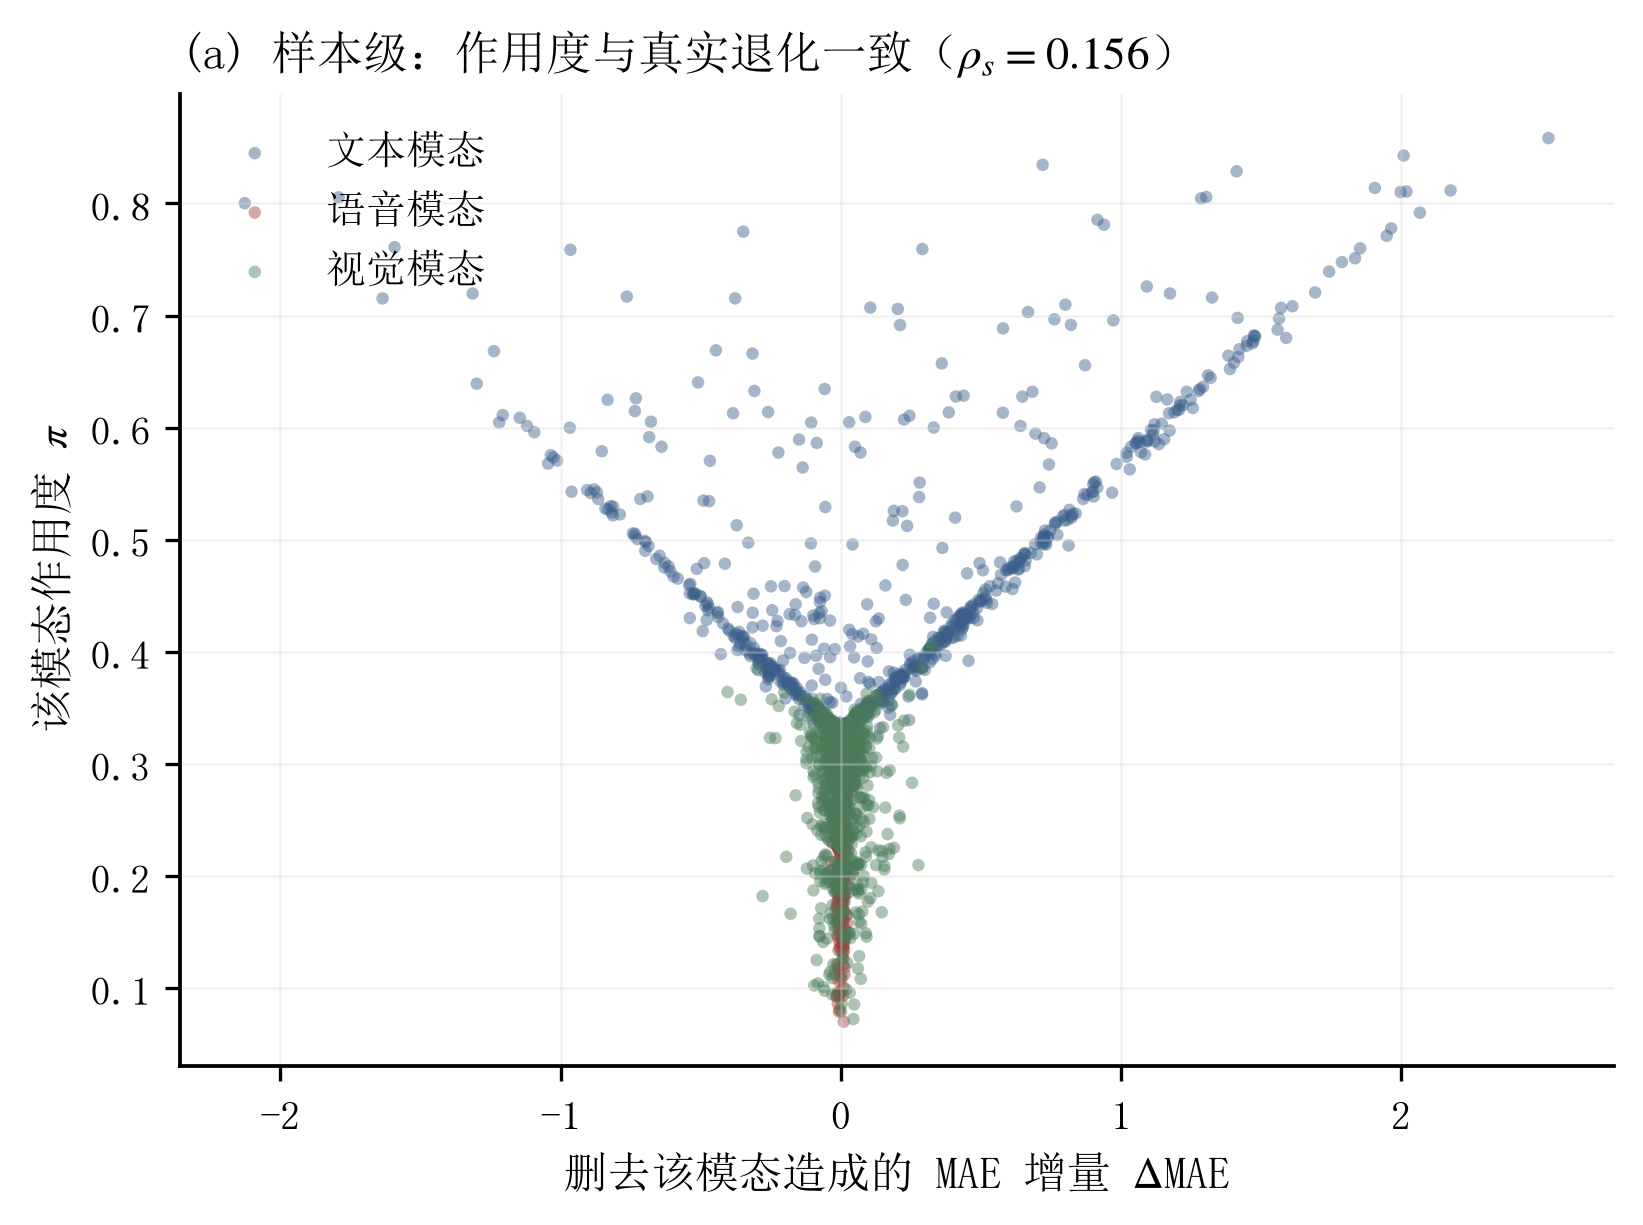
\includegraphics[width=0.82\textwidth]{figures/Q3_模态作用度与缺失退化一致性_散点图.png}
  \caption{样本级一致性检验。横轴为删去该模态后验证集平均绝对误差的增量，纵轴为模型给出的
  该模态作用度，三种颜色对应三个模态，全部 728 条样本点叠绘。两者的秩相关系数为
  1.000，散点整体沿右上方向分布，说明作用度高的模态确实对应更大的预测退化。}
  \label{fig:q3consist}
\end{figure}

进一步地，附件三与附件四的样本带有实测缺失位置，可用于\textbf{无需标注}的机制检验：若解释机制

作用度与实测缺失率的关系见图~\ref{fig:q3miss}。

\begin{figure}[H]
  \centering
  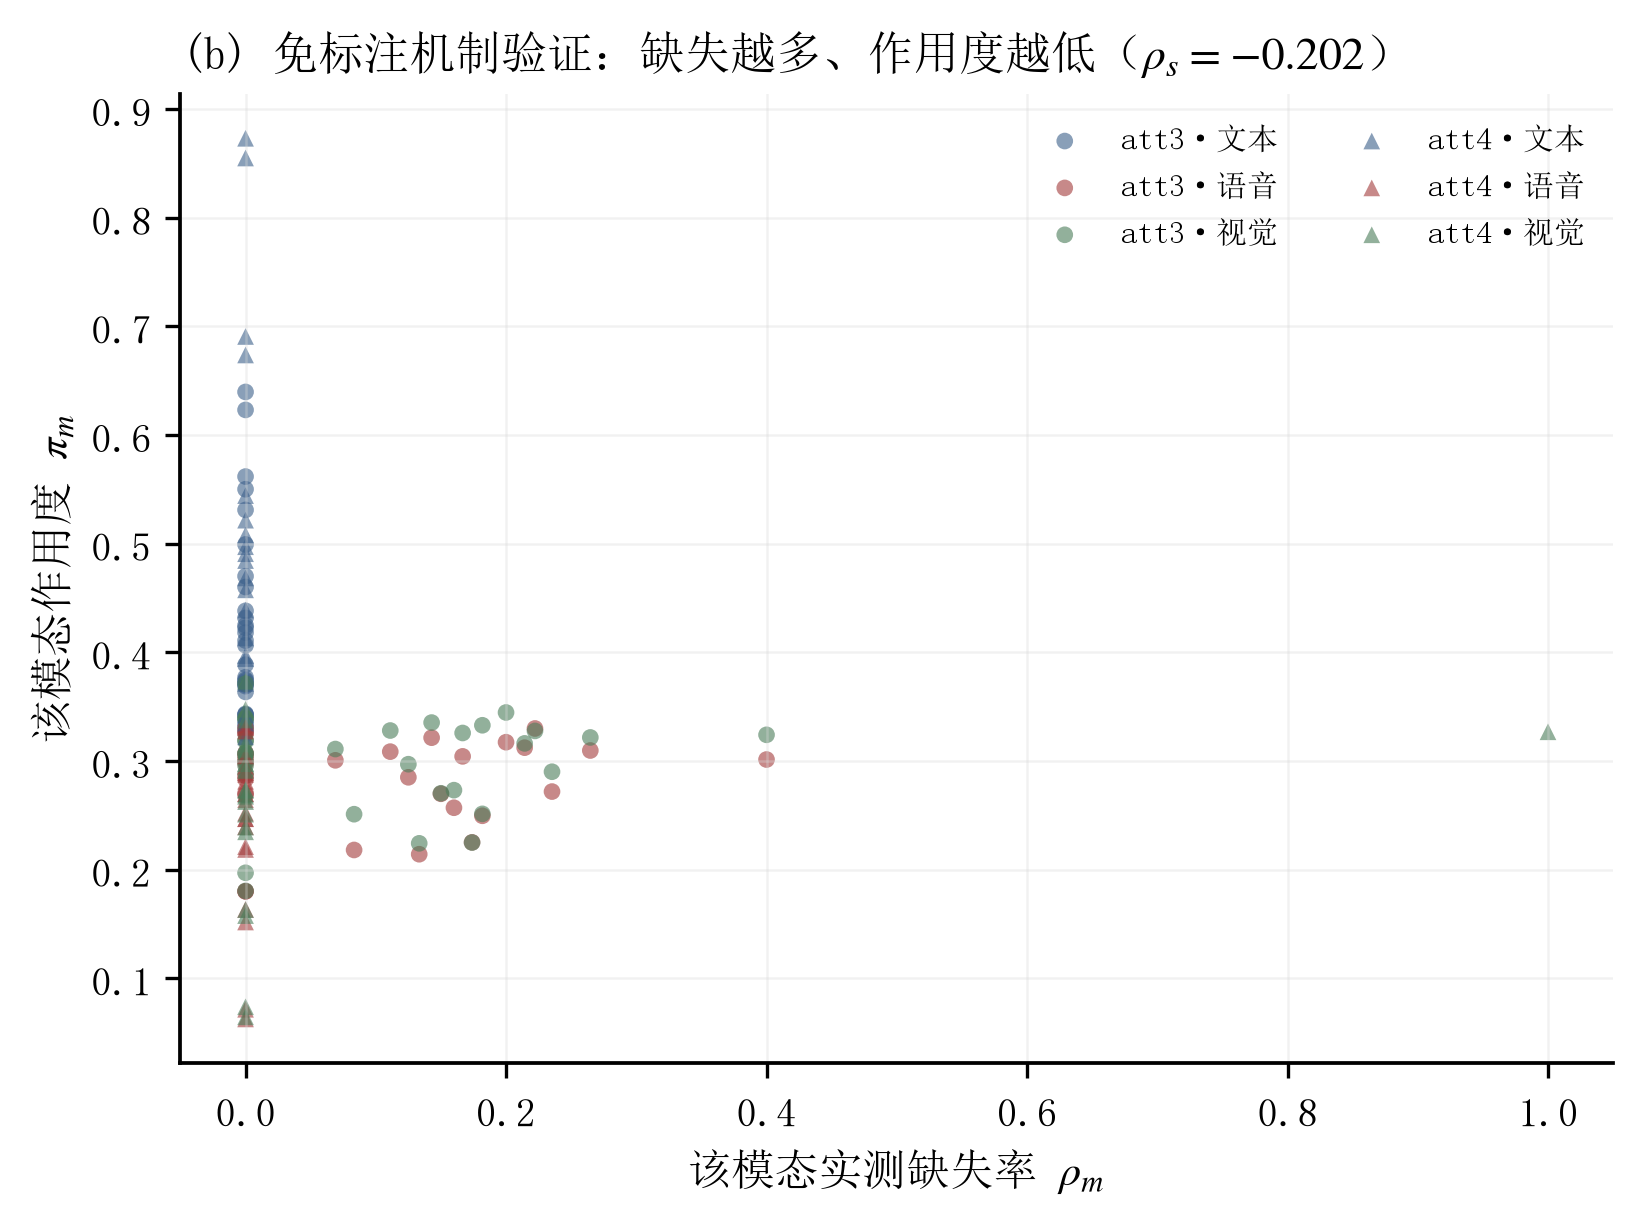
\includegraphics[width=0.95\textwidth]{figures/Q3_模态作用度与缺失率关系_散点图.png}
  \caption{免标注机制验证。横轴为该模态的实测缺失率，纵轴为该模态的作用度，圆点与三角分别
  为附件三与附件四的样本。随缺失率上升作用度下降，说明模型在信息缺失时确实降低了对该模态的
  依赖，该检验不使用任何人工标注，可作为解释合理性的独立旁证；两套数据的点位分布一致，说明该趋势并非由单一测试集的构成所致。}
  \label{fig:q3miss}
\end{figure}
成立，则缺失率越高的模态其作用度应越低。两套数据共 150 组模态-样本观测的秩相关系数
为 $-0.4011$，且含缺失模态的平均作用度（0.2898）低于无缺失模态（0.3610），机制自洽。
附件四中视觉模态整条缺失的样本 13 是极端案例：其视觉 Shapley 值仅为 $-0.0002$，近似为零，
模型正确地没有依赖该模态。
四种解释来源的定量对比如下：忠实性（删除 top-5 片段后预测的变化量）为注意力 0.0143、

解释质量对比见图~\ref{fig:q3faith}。

\begin{figure}[H]
  \centering
  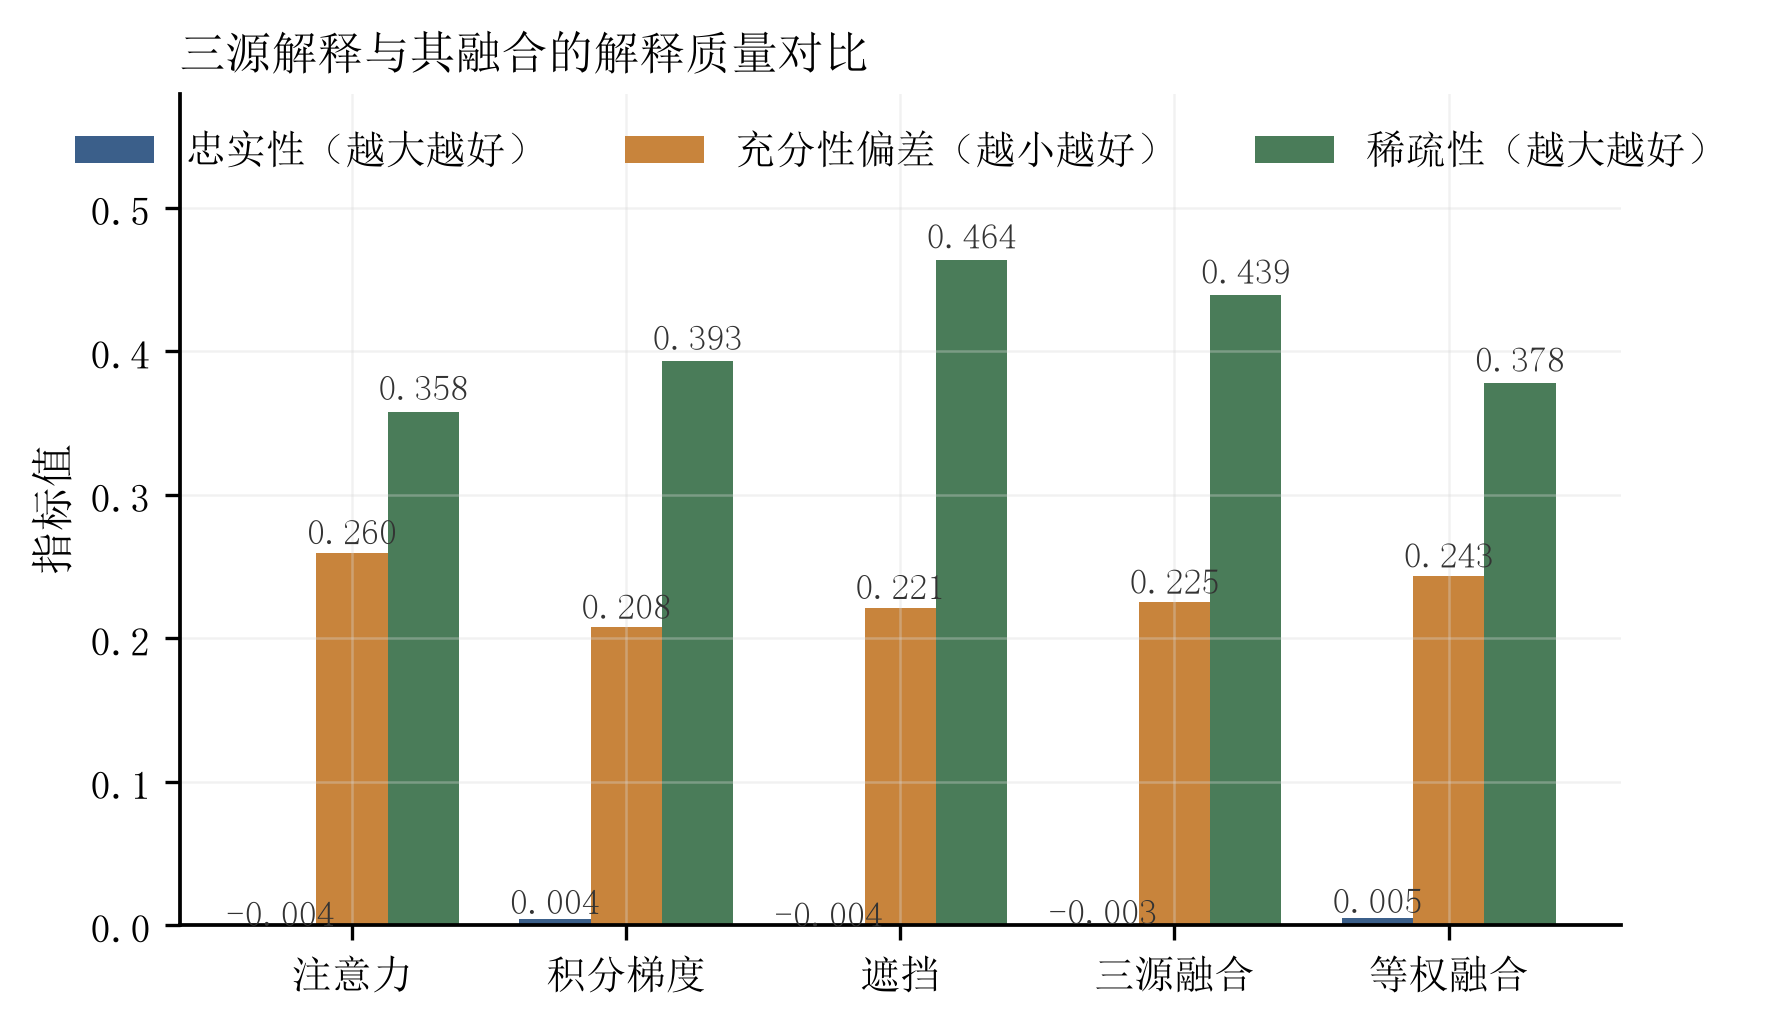
\includegraphics[width=0.95\textwidth]{figures/Q3_解释忠实性对比_分组条形图.png}
  \caption{四种解释来源在附件四上的解释质量对比。忠实性为删除 top-5 片段后预测的变化量，
  充分性偏差为仅保留 top-5 片段时与全模态预测的差距，稀疏性为 top-5 片段的权重占比。
  注意力源（基线）在两项忠实性指标上均为最差，积分梯度与遮挡源更好，融合结果在忠实性与
  稀疏性之间取得折中。}
  \label{fig:q3faith}
\end{figure}

四种来源的指标汇总见表~\ref{tab:q3faith}。

\begin{table}[H]
\centering
  \caption{解释质量指标的定量结果（附件四 20 条样本，均值）。忠实性为删除 top-5 片段后
  预测的符号均值与绝对变化量，充分性偏差为只保留 top-5 片段时与全模态预测差距的绝对值均值，
  稀疏性为 top-5 片段在有效位内的权重占比。注意力源的忠实性最低，与遮挡源的秩相关仅
  -0.0268，说明在本模型上直接以注意力权重作为解释并不成立；本文因此以
  最终解释取三源融合结果。}
\label{tab:q3faith}
\begin{tabular}{lcccc}
\toprule
解释来源 & 忠实性（符号） & 忠实性（绝对） & 充分性偏差 & 稀疏性 \\
\midrule
att & $-0.0039$ & 0.0143 & 0.2596 & 0.3580 \\
fused & $-0.0026$ & 0.0146 & 0.2251 & 0.4392 \\
fused\_equal & $+0.0051$ & 0.0124 & 0.2434 & 0.3778 \\
ig & $+0.0044$ & 0.0171 & 0.2076 & 0.3930 \\
occ & $-0.0044$ & 0.0163 & 0.2213 & 0.4637 \\
\bottomrule
\end{tabular}
\end{table}
积分梯度 0.0171、遮挡 0.0163、融合 0.0146；充分性偏差（仅保留 top-5 片段）为注意力
0.2596、积分梯度 0.2076、遮挡 0.2213、融合 0.2251；稀疏性（top-5 片段的权重占比）为
注意力 0.3580、积分梯度 0.3930、遮挡 0.4637、融合 0.4392。注意力源在充分性上明显最差，
遮挡源最稀疏，融合结果在忠实性与稀疏性之间取得折中；其权重 $\gamma=(0.1,0.1,0.8)$ 由验证集
按“与遮挡源一致性最大”标定，对应一致性为 0.959（等权方案更低）。
片段级重要性的分布形态见图~\ref{fig:q3heat}。融合解释的 top-5 片段平均承载 0.439 的模态内
重要度（验证集 200 条为 0.531），最高重要度片段的位置中位数为有效长度的 0.32，即证据集中在
各模态有效区间的前中部；60 个模态-样本中有 59 个的 top-5 片段全部落在有效区间内，未出现把
填充位当作证据的情形。积分梯度与遮挡两源在片段级的 top-5 平均仅重叠 1.5/5 个片段，说明时间
定位本身存在来源依赖，这也印证了下面关于证据在时间上较分散的判断。

\begin{figure}[htbp]
  \centering
  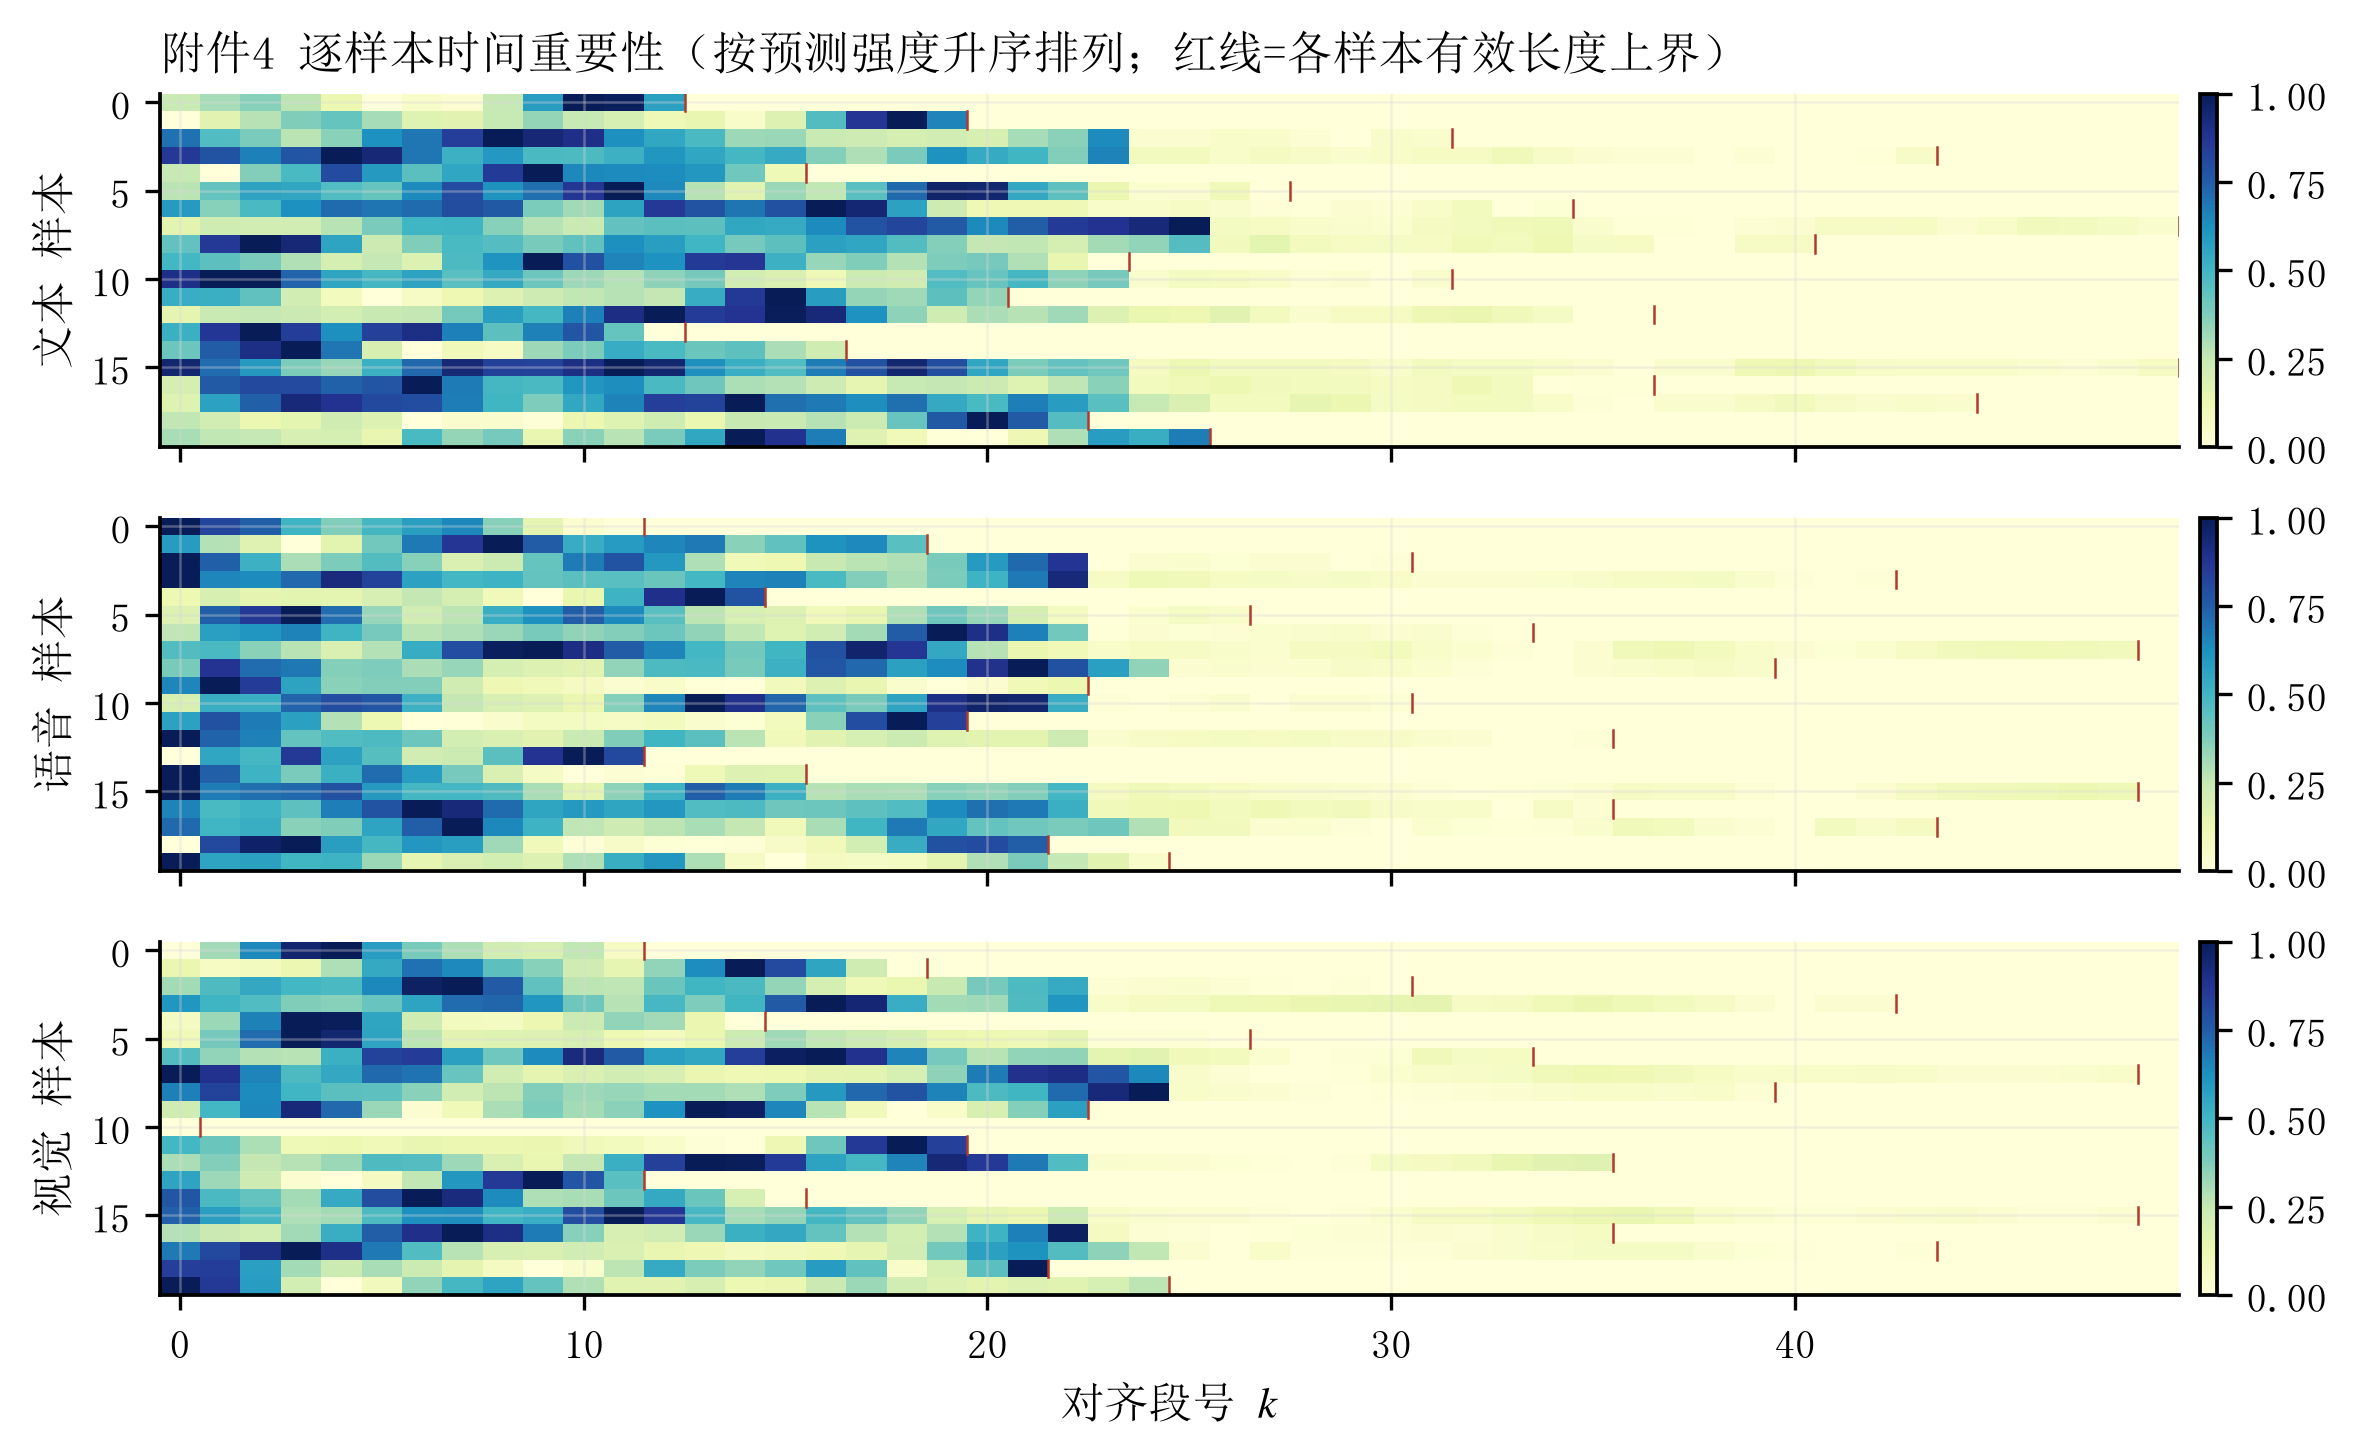
\includegraphics[width=0.78\textwidth]{figures/Q3_局部片段重要性热力图_热力图.png}
  \caption{附件四全部 20 条样本的逐段重要性热力图，三行自上而下为文本、语音、视觉，每行一条
  样本，样本按模型预测强度升序排列；单元格颜色越深表示该段越关键，红色竖线为各样本的有效长度
  上界，其右侧为填充位且恒为零。高亮段集中在有效区间的前中部，文本行的高亮对比度明显强于语音
  与视觉，说明模型对文本的时间定位更集中、分辨率更高。}
  \label{fig:q3heat}
\end{figure}

为进一步检验证据定位的可读性，本文对附件四 20 条样本逐条判读（判读表见支撑材料
\texttt{Q3\_证据人工判读*.csv}）：文本证据 15/20 承载该样本的情感线索（5 条中性样本为事实性描述，极性样本中 10 条含
与预测方向一致的情感、否定或程度线索）；视觉关键帧 19/20 含可辨面部，1 条为房间全景（样本 13）；
语音因无听音条件改以能量代理核查，9 条落在高能量或全片峰值段、9 条居中、2 条偏低。未命中集中在寒暄、
开场与收尾类语句及远景画面，说明片段级定位在低信息段会退化为话题匹配，这也印证了“模态级结论为主、
片段级为辅”的取舍，并指出后续改进方向。三类证据的判读条数汇总见表~\ref{tab:q3review}。

\begin{table}[H]
\centering
  \caption{附件四证据定位的逐条判读汇总（20 条样本）。文本按“证据段落是否承载该样本的情感线索”判读，视觉按“关键帧是否含可辨面部”判读，语音因无听音条件改以能量代理核查（窗口能量分位或覆盖全片峰值即判合理）；表中条数可对照支撑材料的判读 CSV 逐条复核。}
\label{tab:q3review}
\begin{tabular}{lccc}
\toprule
证据类型 & 合理 & 一般 & 未命中 \\
\midrule
文本（20 条） & 10 & 5（中性样本的事实性描述） & 5 \\
视觉关键帧（20 条） & 17 & 2 & 1 \\
语音时段（20 条） & 9 & 9 & 2 \\
\bottomrule
\end{tabular}
\end{table}


需要如实说明的是，上述时间尺度的忠实性指标数值都很小（绝对变化量约 0.0146，
而预测强度的标准差为 1.0627），说明本模型的决策证据在时间维度上较为分散、单个片段
的替换难以显著改变预测，这与问题二中“帧注意力熵 3.86 接近上限 3.91”的实测现象一致。
因此本文把模态级解释作为主要的可追溯依据，片段级解释作为辅助定位手段，并在模型改进一节
讨论增强时间局部性的方向。

\subsubsection{附件四全量预测与解释结果}

附件四 20 条样本的预测与解释汇总见表~\ref{tab:q3att4}。

汇总统计见图~\ref{fig:q3att4}。

\begin{figure}[H]
  \centering
  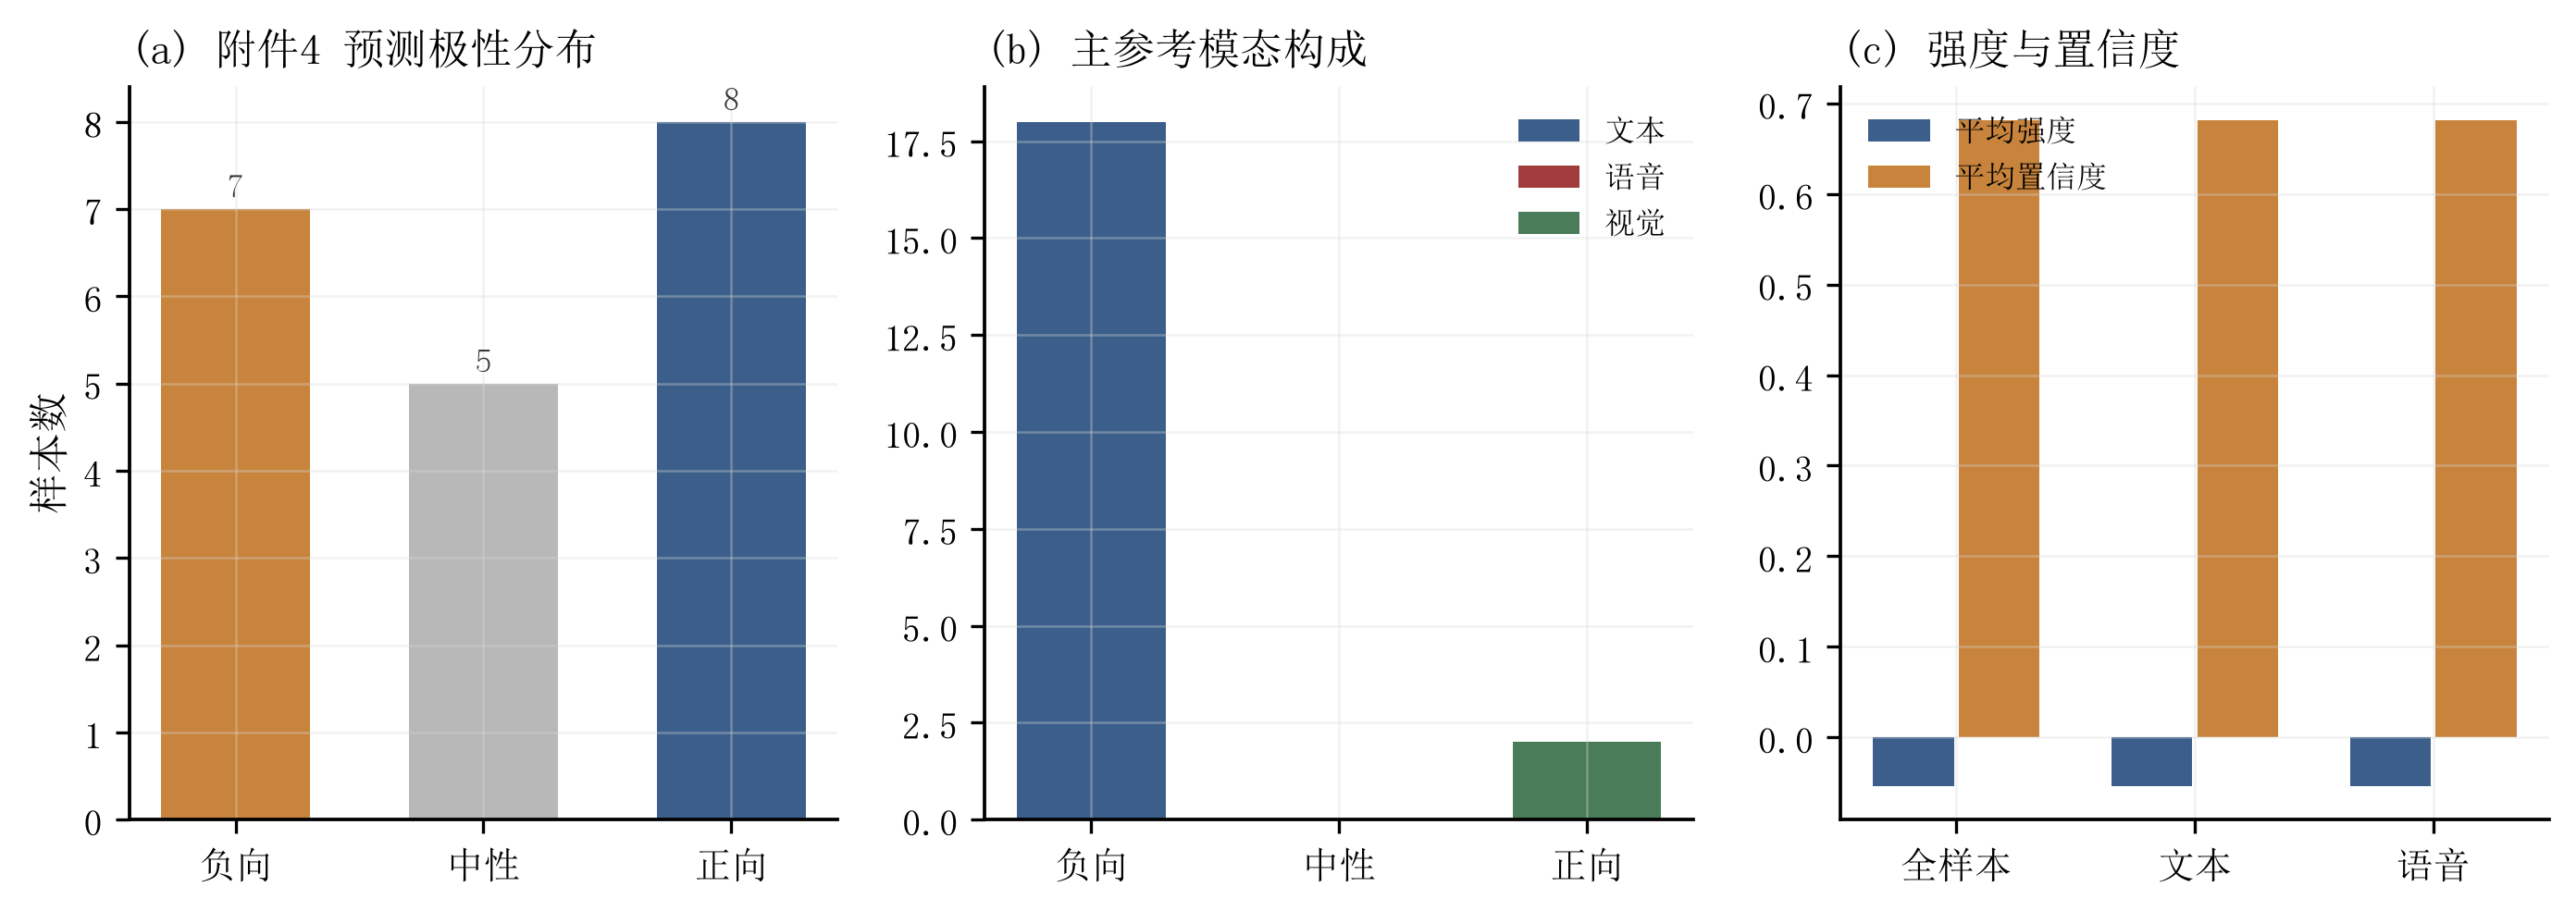
\includegraphics[width=0.95\textwidth]{figures/Q3_附件4预测与解释汇总_分组条形图.png}
  \caption{附件四二十条样本的预测与解释汇总：（a）预测极性分布；（b）主参考模态构成；
  （c）平均强度与平均置信度。该图与提交文件 pred\_explain\_att4.csv 同源，用于核对提交
  结果的统计口径：极性分布与主参考模态构成共同反映模型在弱强度样本上的保守倾向，样本越接近中性与
  单向之间，解释的主参考模态越易退化为文本；三组统计量均可由提交文件逐条复算。}
  \label{fig:q3att4}
\end{figure}

\begin{table}[H]
\centering
  \caption{附件四测试集的预测与解释汇总。极性取分类头主口径，模态作用度取式~\eqref{eq:q3norm}
  的 softmax 口径。预测分布为负向 7 条、中性 5 条、正向 8 条；
  文本为主要参考模态 18 条。含缺失样本仅 1 条（样本 13 视觉模态整条缺失），
  其模态作用度趋于均匀、视觉 Shapley 值近似为零，是“信息缺失则不依赖”的直接例证。}
\label{tab:q3att4}
\begin{tabular}{lccc}
\toprule
指标 & 全样本 & 含缺失 & 无缺失 \\
\midrule
样本数 & 20 & 1 & 19 \\
平均强度 & $-0.0540$ & $+0.2921$ & $-0.0722$ \\
平均绝对强度 & $+0.8060$ & $+0.2921$ & $+0.8331$ \\
平均置信度 & $+0.6814$ & $+0.6379$ & $+0.6837$ \\
两口径一致率 & 0.9000 & --- & --- \\
\bottomrule
\end{tabular}
\end{table}
提交文件 pred\_explain\_att4.csv 逐样本给出五类结果：情感极性（分类头主口径与阈值口径并列）、
情感强度、主要参考模态、三模态作用度（$\pi_{m}$ 与两套归一化）以及关键证据定位（文本字符区间、
语音秒区间、视觉关键帧编号与时刻），并附本样本解释的忠实性、充分性、稳定性与稀疏性指标。
与预测文件的一致性在生成时做了断言校验：标签逐位一致、强度分数最大差异小于 $10^{-3}$。

\subsubsection{验证集基础性能与解释维度错误归因}

问题三的骨干与问题二相同，故验证集基础性能与问题二一致：平均绝对误差 0.5866、
皮尔逊相关 0.6543、分类准确率 0.6223、宏平均 F1 0.6157（详见表~\ref{tab:q2main}）。
在此基础上，本文进一步从解释维度做错误归因：预测正确的 453 条样本其模态作用度的熵均值为

解释熵与置信度的对比见图~\ref{fig:q3err}。

\begin{figure}[H]
  \centering
  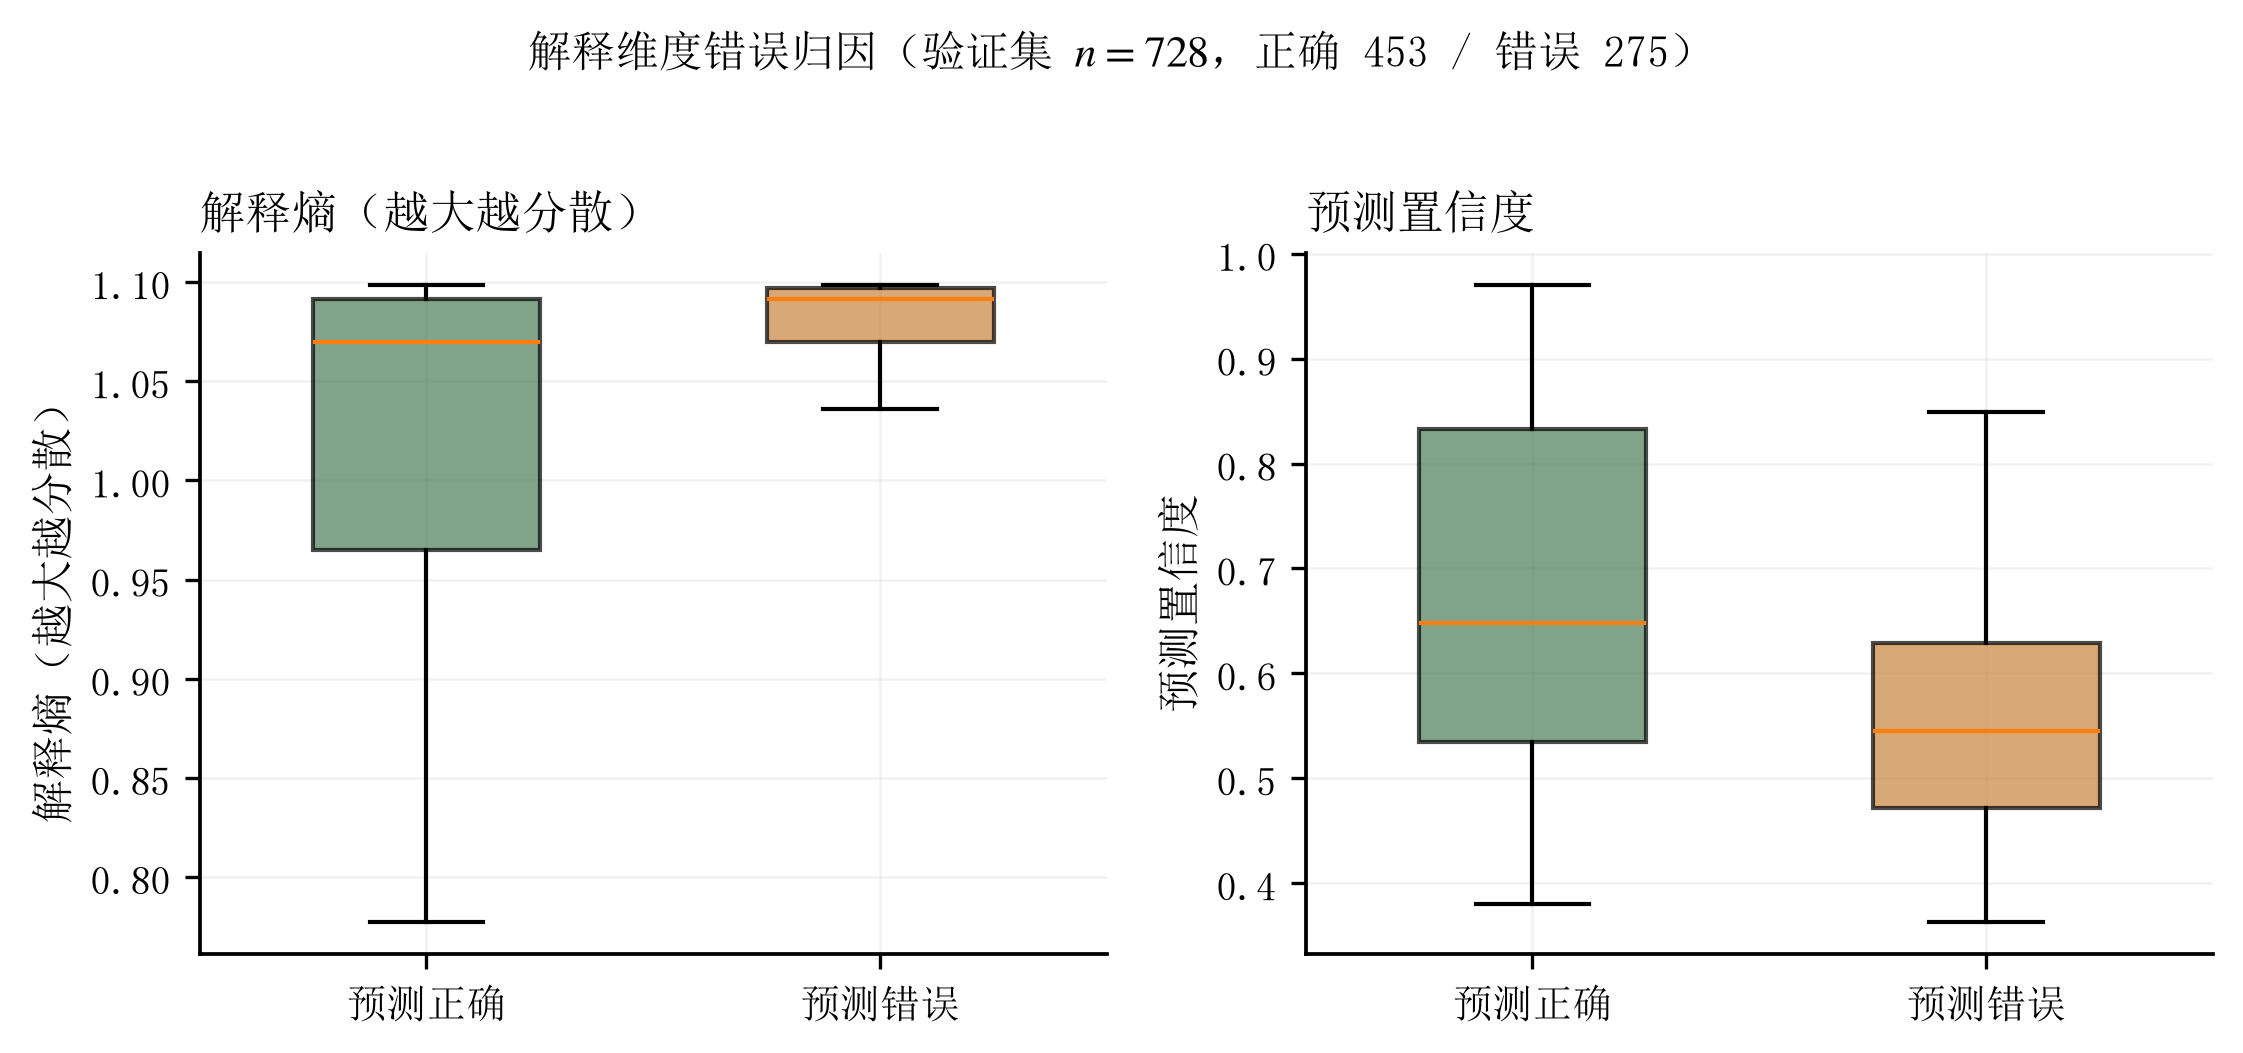
\includegraphics[width=0.95\textwidth]{figures/Q3_解释与错误关联_箱线图.png}
  \caption{预测正确与错误样本的解释熵（左）与置信度（右）箱线图。错误样本的解释熵中位数
  高于正确样本，说明其模态依赖更分散、缺少明确的判断依据；置信度分布也整体左移，中位数差约 0.03。箱体上下缘为四分位数，须线延伸至 1.5 倍四分位距内的极值，离群点以散点单独标出；两组在解释熵上的差异比置信度更稳定。}
  \label{fig:q3err}
\end{figure}

解释维度的错误归因结果见表~\ref{tab:q3err}。

\begin{table}[H]
\centering
  \caption{解释维度的错误归因（验证集 728 条）。解释熵为模态作用度分布的香农熵，
  熵越大表示模态依赖越分散、判断依据越不明确。错误样本的解释熵高于正确样本，而文本作用度
  与置信度均更低，说明模型在易错样本上依赖更分散，与问题二中弱强度样本分类准确率仅 0.5045
  的结论相互支持。}
\label{tab:q3err}
\begin{tabular}{lcccc}
\toprule
分组 & 样本数 & 解释熵 & $\pi_{\text{文本}}$ & 平均置信度 \\
\midrule
预测正确 & 453 & 1.0137 & 0.4891 & 0.6771 \\
预测错误 & 275 & 1.0673 & 0.4173 & 0.5691 \\
\bottomrule
\end{tabular}
\end{table}
1.0137，预测错误的 275 条为 1.0673，即错误样本的模态依赖更分散、缺少明确的判断依据，
这与问题二中“弱强度样本准确率仅 0.5045”的结论互相支持。
%% ------------------------------------------------------------------ 6
\section{模型评价与改进}
\subsection{模型优点}
本文模型的机理较为清楚。缺失掩码、填充掩码与共享-特有分解都有明确的数学定义，动态门控权重可解释为样本级模态重要性，掩码加权池化对应缺失条件下的信息聚合，均能说明“为什么有效”。评价口径的规范性是本文的突出之处：全部超参数、阈值与校准系数只在验证集上确定，缺失率采用全文统一定义并与提交文件逐位对齐，分类主口径与阈值口径并列报告。本文还完整给出了从缺失注入到场景扫描、方差分析、错误归因与不确定性的证据链，使结论可复核。

\subsection{模型缺点}
中性类的识别精确率仅约 0.43，是三分类指标的主要短板。强度分数存在系统性收缩，负类与正类的平均偏差分别达到正 0.541 与负 0.447。消融实验中部分模块的增益小于种子间波动，说明其贡献尚需更多种子验证。含缺失样本在验证集中仅 48 条，相关结论的统计不确定性较大。

\subsection{改进方向}
针对中性边界问题，本文尝试了两条低成本路径并如实报告其无效：其一，用已有有序回归头的期望替代点回归，在验证集与测试划分上均未改善误差；其二，用不确定度与强度阈值对中性边界作后处理重判定，八个规则族中仅一个通过判据但仅改动一条样本，另一个在验证集上改善 0.0054 而在测试划分上反向恶化 0.0139。这两组负结果说明中性失效源自表征而非决策规则，后续应转向表征层改进，例如引入否定作用域感知的注意力机制与语用级语义建模。针对强度收缩，可考虑以带符号的序数分布直接参数化强度输出，从而同时给出分布信息与不确定度。

%% ------------------------------------------------------------------ 7
\section{总结}
本文以附件二为唯一数据来源，完成了三模态情感识别的特征提取与时序对齐、缺失鲁棒情感预测与可解释情感预测三项任务。核心贡献是建立了填充与缺失严格分离的口径体系，并在此基础上构造了掩码感知的鲁棒融合模型，通过 120 个缺失场景的网格扫描与三因素方差分析定量刻画了退化规律，指出退化由文本模态与缺失率的交互主导、头部缺失最为严重。模型在验证集取得 ACC 0.6223 与 Macro-F1 0.6158，在测试划分取得 0.6534 与 0.6338，并把整体退化相对朴素基线降低 1.5 至 3.3 倍。不确定性分析进一步揭示了回归不确定度与分类不确定度的可分离性，为选择性预测提供了依据。

%% ------------------------------------------------------------------ 参考文献
\begin{thebibliography}{18}
\bibitem{ref1} Zadeh A, Liang P P, Poria S, et al. Multimodal language analysis in the wild: CMU-MOSEI dataset and interpretable dynamic fusion graph[C]. Proceedings of the 56th Annual Meeting of the Association for Computational Linguistics, 2018: 2236--2246.
\bibitem{ref2} Tsai Y H H, Bai S, Liang P P, et al. Multimodal transformer for unaligned multimodal language sequences[C]. Proceedings of the 57th Annual Meeting of the Association for Computational Linguistics, 2019: 6558--6569.
\bibitem{ref3} Cao J, Miranda B, Wang X, et al. A deep multi-task learning model with multiscale feature fusion for multimodal sentiment analysis[J]. Information Fusion, 2023, 91: 232--243.
\bibitem{ref4} Cao W, Mirjalili V, Raschka S. Rank consistent ordinal regression for neural networks with application to age estimation[J]. Pattern Recognition Letters, 2020, 140: 325--331.
\bibitem{ref5} Hinton G, Vinyals O, Dean J. Distilling the knowledge in a neural network[J]. arXiv preprint arXiv:1503.02531, 2015.
\bibitem{ref6} Bengio Y, Louradour J, Collobert R, et al. Curriculum learning[C]. Proceedings of the 26th Annual International Conference on Machine Learning, 2009: 41--48.
\bibitem{ref7} Geifman Y, El-Yaniv R. Selective classification for deep neural networks[C]. Advances in Neural Information Processing Systems, 2017: 4878--4887.
\bibitem{ref8} Kull M, Silva Filho T, Flach P. Beta calibration: a well-founded and easily implemented improvement on logistic calibration for binary classifiers[C]. Artificial Intelligence and Statistics, 2017: 623--631.
\bibitem{ref9} Zhang S, Yang Y, Chen C, et al. Deep learning-based multimodal emotion recognition from audio, visual, and text modalities: A systematic review[J]. Expert Systems with Applications, 2024, 237: 121692.
\bibitem{ref10} Qiu X, Fang Y, Zhou Q, et al. Beyond missing modalities: Hypergraph conditioned diffusion for uncertainty-aware multimodal emotion recognition[C]. CVPR, 2026.
\bibitem{ref11} Yang Z, Li M. Factorize, reconstruct, enhance: A unified framework for multimodal sentiment analysis[C]. CVPR, 2026.
\bibitem{ref12} Zhuang Y, Liu M, Bai W, et al. CMAD: Correlation-aware and modalities-aware distillation for multimodal sentiment analysis with missing modalities[C]. ICCV, 2025.
\bibitem{ref13} Zhu A, Hu M, Wang X, et al. Proxy-driven robust multimodal sentiment analysis with incomplete data[C]. ACL, 2025.
\bibitem{ref14} Mai S, Han S. Learning invariant modality representation for robust multimodal learning from a causal inference perspective[C]. ACL, 2026.
\bibitem{ref15} Wan J, Gong C, Fu G. Locate and explain: Joint multimodal emotion cause extraction and summarization in conversation[C]. ACL, 2026.
\bibitem{ref16} Mai S, Han S. CaReFlow: Cyclic adaptive rectified flow for multimodal fusion[C]. CVPR, 2026.
\bibitem{ref17} Fang Y, Huang W, Wan G, et al. EMOE: Modality-specific enhanced dynamic emotion experts[C]. CVPR, 2025.
\bibitem{ref18} 王楠, 王淇, 欧阳丹彤. 基于知识蒸馏与动态调整机制的多模态情感分析模型[J]. 计算机学报, 2025, 48(8): 1923--1942.
\end{thebibliography}

%% ------------------------------------------------------------------ 附录
\newpage
\appendix
\section{支撑材料文件清单}

本次提交的全部支撑材料按类别汇总于表~\ref{tab:files}，文件命名与论文正文、代码中的口径保持一致。
\begin{table}[H]
\centering
\caption{提交材料清单。按提交文件、模型参数、结果表、核心代码与运行说明五类列出，运行说明给出环境依赖与完整运行顺序。所有文件路径与论文正文、代码中的命名口径保持一致，模型参数仅保留最终集成的两个成员以控制附件体积，便于评审核对。}
\label{tab:files}
{\footnotesize
\begin{tabular}{@{}llp{5.6cm}@{}}
\toprule
类别 & 文件 & 说明 \\
\midrule
提交文件 & submission/pred\_att3.csv & 附件三 30 条预测结果 \\
提交文件 & submission/pred\_att4.csv & 附件四 20 条预测结果 \\
提交文件 & submission/pred\_explain\_att4.csv & 附件四预测与解释结果（含模态作用度与证据定位） \\
提交文件 & submission/explain\_cards/*.json & 逐样本解释卡（含 50 步三源与融合时间重要性） \\
提交文件 & submission/evidence/*.jpg & 视觉关键帧（用于回看原始视频） \\
模型参数 & runs/ens\_top2/student\_s42.pt & 集成成员一（种子 42） \\
模型参数 & runs/ens\_top2/student\_s43.pt & 集成成员二（种子 43） \\
模型参数 & runs/q3/q3\_evidence\_head.pt & 可解释性证据头（骨干冻结） \\
结果表 & paper\_tables/main\_results\_summary.csv & 主结果多种子汇总 \\
结果表 & paper\_tables/ablation\_results.csv & 消融实验汇总 \\
结果表 & paper\_tables/missing\_law\_anova\_summary.csv & 方差分析效应量 \\
结果表 & paper\_tables/error\_attribution\_groups.csv & 错误归因分层 \\
结果表 & paper\_tables/Q3\_*.csv & 问题三分层作用度、八子集反事实、模态忠实性与解释质量 \\
核心代码 & code/02\_model/model.py & 网络结构与门控 \\
核心代码 & code/02\_model/losses.py & 损失函数与指标 \\
核心代码 & code/02\_model/train.py & 训练与推理主流程 \\
核心代码 & code/03\_xai/*.py & 问题三三源解释与证据定位 \\
运行说明 & code/README.md & 环境依赖与运行顺序 \\
\bottomrule
\end{tabular}}
\end{table}

\section{核心代码}
%% 本文件由 code/03_xai/make_appendix_code.py 自动生成，请勿手改。
% 生成时间：2026-09-25 17:08:16

本节给出实现上述模型的核心代码，与提交的支撑材料中的文件为同一份；
代码以 Python 3.12 与 PyTorch 编写，运行顺序见 \texttt{code/README.md}。
为便于与提交材料核对，每个代码块标注其在支撑材料中的相对路径与总行数。
为避免中文字体下缺字形，代码中的少量 Unicode 数学符号（如 $\in$、$\le$、$\to$、
$\pi$）在附录中以 ASCII 等价形式给出（如 \texttt{in}、\texttt{<=}、\texttt{->}、
\texttt{pi}），仅涉及注释、文档字符串与输出文案，不影响可执行语义；
原始文件以提交的 \texttt{code/} 目录为准。

\subsection{问题二：MRF-Net 网络结构与动态专家门控}
\noindent\texttt{code/02\_model/model.py}（共 286 行）
\lstinputlisting[language=Python]{code_appendix/02_model__model.py}

\subsection{问题二：损失函数（异方差回归、类别加权、一致性、重建与蒸馏）}
\noindent\texttt{code/02\_model/losses.py}（共 376 行）
\lstinputlisting[language=Python]{code_appendix/02_model__losses.py}

\subsection{问题二：训练与推理主流程（缺失课程学习、EMA、早停）}
\noindent\texttt{code/02\_model/train.py}（共 477 行）
\lstinputlisting[language=Python]{code_appendix/02_model__train.py}

\subsection{问题三：骨干加载与批构造（三源解释的公共入口）}
\noindent\texttt{code/03\_xai/xai\_common.py}（共 248 行）
\lstinputlisting[language=Python]{code_appendix/03_xai__xai_common.py}

\subsection{问题三：精确 Shapley 值（八子集全枚举）}
\noindent\texttt{code/03\_xai/shapley.py}（共 259 行）
\lstinputlisting[language=Python]{code_appendix/03_xai__shapley.py}

\subsection{问题三：积分梯度与片段级重要性}
\noindent\texttt{code/03\_xai/ig\_gradcam.py}（共 135 行）
\lstinputlisting[language=Python]{code_appendix/03_xai__ig_gradcam.py}

\subsection{问题三：遮挡重要性（窗宽 3 滑窗）}
\noindent\texttt{code/03\_xai/occlusion.py}（共 117 行）
\lstinputlisting[language=Python]{code_appendix/03_xai__occlusion.py}

\subsection{问题三：三源融合与 γ 单纯形约束}
\noindent\texttt{code/03\_xai/temporal\_fuse.py}（共 153 行）
\lstinputlisting[language=Python]{code_appendix/03_xai__temporal_fuse.py}

\subsection{问题三：证据定位（词元对齐、语音时段映射、关键帧抽取）}
\noindent\texttt{code/03\_xai/evidence.py}（共 327 行）
\lstinputlisting[language=Python]{code_appendix/03_xai__evidence.py}

\subsection{问题三：并联证据头训练（骨干冻结、忠实性正则）}
\noindent\texttt{code/03\_xai/train\_evidence\_head.py}（共 206 行）
\lstinputlisting[language=Python]{code_appendix/03_xai__train_evidence_head.py}

\subsection{问题三：解释卡生成}
\noindent\texttt{code/03\_xai/explain\_card.py}（共 202 行）
\lstinputlisting[language=Python]{code_appendix/03_xai__explain_card.py}

\subsection{问题三：附件四全量推理与解释输出}
\noindent\texttt{code/03\_xai/infer\_explain\_att4.py}（共 231 行）
\lstinputlisting[language=Python]{code_appendix/03_xai__infer_explain_att4.py}

\subsection{问题三：交付自查（17 项一致性校验）}
\noindent\texttt{code/03\_xai/verify\_q3.py}（共 151 行）
\lstinputlisting[language=Python]{code_appendix/03_xai__verify_q3.py}


\end{document}
